%%%%%%%%%%%%%%%%%%%%%%%%%%%%%%%%%%%%%%
% Cahier d'exercices de Colles pour PTSI
%
% olivier.leveque@ens-paris-saclay.fr 
%	http://perso.crans.org/oleveque
%

%%%%%%%%%%%%%%%%%%% EN-TÊTE
%----------------------------------------------------------------------------------------
%	PACKAGES & CONFIGURATIONS
%----------------------------------------------------------------------------------------

\documentclass{report}

\usepackage{fancyhdr} %Custom headers
\usepackage[Rejne]{fncychap} %Custom chapters
	%Options: Sonny, Lenny, Glenn, Conny, Rejne, Bjarne, Bjornstrup

\usepackage{lastpage} %Permet de déterminer quelle est la  dernière pasge du footer

\usepackage[print]{setting/colles-pck} %Styles exos/corrections
	%Options : print = affiche la correction; no-print = n'affiche pas la correction

\usepackage{amssymb} %Symboles spéciaux
\usepackage{extramarks} %Requis pour les headers and footers
\usepackage{graphicx} %Requis pour insérer des images
\usepackage{amsmath} %Texte dans les expressions mathématiques
\usepackage{calligra}
\usepackage{pdfpages} %Permet d'importer des documents PDF
\usepackage[labelsep=quad,indention=10pt]{subfig}
\captionsetup*[subfigure]{position=bottom}

\usepackage[utf8]{inputenc}
\usepackage[francais]{babel} %Langue Française
\usepackage[pdftex]{hyperref}

%Configurations du PDF
\hypersetup{
    bookmarks=true,         % show bookmarks bar?
    unicode=false,          % non-Latin characters in Acrobat’s bookmarks
    pdftoolbar=true,        % show Acrobat’s toolbar?
    pdfmenubar=true,        % show Acrobat’s menu?
    pdffitwindow=true,      % page fit to window when opened
    pdftitle={Khôlles de Sciences Industrielles},    % title
    pdfauthor={Olivier Lévêque},     % author
    pdfsubject={Exercices oraux de Sciences Industrielles pour PTSI},   % subject of the document
    pdfnewwindow=true,      % links in new window
    pdfkeywords={khôlles} {colles} {exercices} {oral} {corrections} {PTSI} {Sciences Industrielles} {Classes Préparatoires} {CPGE} {Ginette} {Lycée Sainte-Geneviève} {Versailles} {SI} {SII} {Banque PT}, % list of keywords
    colorlinks=false,       % false: boxed links; true: colored links
    linkcolor=red,          % color of internal links
    citecolor=green,        % color of links to bibliography
    filecolor=magenta,      % color of file links
    urlcolor=cyan           % color of external links
}

%Mise en page (marges)
\topmargin=-0.45in
\evensidemargin=0in
\oddsidemargin=0in
\textwidth=6.5in
\textheight=9.0in
\headsep=0.25in 

\linespread{1.1} %Espace entre les lignes

%----------------------------------------------------------------------------------------
%	DOCUMENT STRUCTURE COMMANDS
%----------------------------------------------------------------------------------------

\newcommand*{\plogo}{\fbox{$\mathcal{BJ}$}} %Logo générique

\newcommand{\email}[1]{\href{mailto:#1}{\nolinkurl{#1}}} %Hyperlien pour les adresses emails

\newcommand{\blankpage}{
	\newpage
	\null % Insérer une page vierge
	\thispagestyle{empty} % Supprimer le header & le footer sur cette page
	\newpage}

\setcounter{secnumdepth}{1} %Supprimer la numérotation par défaut des subsections

%----------------------------------------------------------------------------------------
%	CONFIGURATIONS HEADER & FOOTER
%----------------------------------------------------------------------------------------

\newcommand{\hdTitle}{Classes préparatoires en Physique, Technologie et Sciences de l'Ingénieur du Lycée Sainte-Geneviève} %Titre du header

%Set up du header et du footer
\pagestyle{fancy}
\lhead{} %Top left header
\chead{\hdTitle} % Top center header
\rhead{} %Top right header
\lfoot{\hyperref[sommaire]{$\diamondsuit$}} %Bottom left footer
\cfoot{} %Bottom center footer
\rfoot{Page\ \thepage\ de\ \pageref{LastPage}} %Bottom right footer
\renewcommand\headrulewidth{0.4pt} %Size of the header rule
\renewcommand\footrulewidth{0.4pt} %Size of the footer rule

\setlength\parindent{0pt} %Supprime toutes indentations venant des paragraphes


%----------------------------------------------------------------------------------------
%	CONFIGURATION PAGE TITLE
%----------------------------------------------------------------------------------------
\newcommand*{\couverture}{
\begingroup % Create the command for including the title page in the document
\centering % Center all text

\vspace*{\baselineskip} % White space at the top of the page
\rule{\textwidth}{1.6pt}\vspace*{-\baselineskip}\vspace*{2pt} % Thick horizontal line
\rule{\textwidth}{0.4pt}\\[\baselineskip] % Thin horizontal line

{\LARGE KHÔLLES DE \\[0.3\baselineskip] SCIENCES INDUSTRIELLES}\\[0.2\baselineskip] % Title

\rule{\textwidth}{0.4pt}\vspace*{-\baselineskip}\vspace{3.2pt} % Thin horizontal line
\rule{\textwidth}{1.6pt}\\[\baselineskip] % Thick horizontal line

\scshape % Small caps
Exercices pour les classes pr\'eparatoires en \\ % Tagline(s) or further description
Physique, Technologie et Sciences de l'Ing\'enieur \\ % Tagline(s) or further description
du Lyc\'ee Sainte-Genevi\`eve \\[\baselineskip] % Tagline(s) or further description
Versailles,  2014--2016\par % Location and year

\vspace*{2\baselineskip} % Whitespace between location/year and editors

\'Ecrit par \\[\baselineskip]
{\Large OLIVIER LÉV\^EQUE \par} % Editor list
{\itshape \'El\`eve\ Normalien\par} % Editor affiliation

\vfill % Whitespace between editor names and publisher logo

%\plogo \\[0.3\baselineskip] % Publisher logo
\href{http://wwww.bginette.com}{
\includegraphics[scale=0.3]{png/logo.png}}\\
\href{http://wwww.bginette.com}{{\scshape Ginette}} \\[0.3\baselineskip] % Version

\endgroup
}

%%%%%%%%%%%%%%%%%%% DOCUMENT
\begin{document}
%----------------------------------------------------------------------------------------
%	COUVERTURE
%----------------------------------------------------------------------------------------

\thispagestyle{empty} %Supprimer le header & le footer sur cette page
\couverture

\newpage

%----------------------------------------------------------------------------------------
%	CONTENUS
%----------------------------------------------------------------------------------------
%----------------------------------------------------------------------------------------
%	AVANT-PROPOS
%----------------------------------------------------------------------------------------

\chapter*{Avant-Propos}
\paragraph{}
Ce cahier d'exercices est destiné aux examens oraux hebdomadaires de Sciences Industrielles pour l'ingénieur. Il est composé de $8$ chapitres s'appuyant sur le programme officiel des classes préparatoires de Physique, Technologie, et Sciences de l'Ingénieur.

\paragraph{}
Il est confié aux lecteurs la tâche de retourner remarques et suggestions, afin d'améliorer cet ouvrage, en utilisant le courier électronique à l'adresse : \textit{\email{olivier.leveque@ens-cachan.org}}.

\vfill 
\begin{flushright}
\textit{
	Écrit le 17 octobre 2014, à Cachan,\\
	Actualisé le \today.}
\end{flushright}
\thispagestyle{empty} %Supprimer le header & le footer sur cette page
\newpage

%----------------------------------------------------------------------------------------
%	TABLE DES MATIÈRES
%----------------------------------------------------------------------------------------

%\setcounter{tocdepth}{1} % Décommenter cette ligne pour ne pas faire apparaître les subsections

{\pagestyle{plain} % Supprimer le header & le footer sur cette page en laissant la numérotation
\setcounter{page}{1}

%\renewcommand{\contentsname}{Sommaire} % Renommer le titre de la table des matières
\tableofcontents\label{sommaire} %lien interne vers tableofcontents
\newpage} % Introduction
\setcounter{page}{1}

\chapter{Systèmes Linéaires, Continus et Invariants}
\thispagestyle{plain} % Supprimer le header & le footer sur cette page en laissant la numérotation
\newpage

%----------------------------------------------------------------------------------------
%	Transformées de Laplace
%----------------------------------------------------------------------------------------

\section{Transformées de Laplace}

%--------------------------------------------

\exercice{Transformées de Laplace inverses et directes}

\subsubsection{PARTIE 1}
Calculez la r\'eponse impulsionnelle \`a un dirac unitaire des syst\`emes caract\'eris\'es par les fonctions de transfert suivantes :

\begin{enumerate}
\item \(H(p) = \frac{p+1}{p^2+5p+6}\)
\item \(H(p) =\frac{p+1}{p^3+3p^2}\)
\item \(H(p) =\frac{1}{p^2+2p+2}\)
\end{enumerate}

\subsubsection{PARTIE 2}
Soit la fonction suivante. On demande de d\'eterminer la transform\'ee de Laplace
de celle-ci :
\begin{enumerate}
\item \(e(t) = [t^2+t-e^{-3t}]\mathcal{U}(t)\)
\item \(e(t) = (t+2)\mathcal{U}(t)+(t+3)\mathcal{U}(t-2)\)
\item \(e(t) = [(t^2+t+1)e^{-2t}]\mathcal{U}(t)\)
\end{enumerate}

\correction{ % Answer
\subsubsection{PARTIE 1}
\begin{enumerate}
\item Comme \( H(p)=\frac{p+1}{(p+2)(p+3)}=\frac{-1}{p+2}+\frac{2}{p+3} \) (racines réelles), \fbox{\(s(t)= [2\exp(-3t)-\exp(-2t)]\mathcal{U}(t)\)}
\item Comme \( H(p)= \frac{p+1}{p^2(p+3)}=\frac{\frac{1}{3}}{p^2}+\frac{\frac{2}{9}}{p}+\frac{-\frac{2}{9}}{p+3} \) (racines doubles), \fbox{\(s(t)= [\frac{1}{3}t+\frac{2}{9}-\frac{2}{9}\exp(-3t)]\mathcal{U}(t)\)}
\item Comme \( H(p)=\frac{1}{(p+1)^2+1} \) (racines complexes), \fbox{\(s(t)= [\sin(t)\exp(-t)]\mathcal{U}(t)\)}
\end{enumerate}

\subsubsection{PARTIE 2}
\begin{enumerate}
\item \fbox{\(E(p) = \frac{2}{p^3}+\frac{1}{p^2}-\frac{1}{p+3}\)}
\item \fbox{\(E(p) = \frac{2p+1}{p^2}+(\frac{1}{p^2}+\frac{5}{p})e^{-2p}\)}
\item \fbox{\(E(p) = \frac{p^2+5p+8}{(p+2)^3}\)}
\end{enumerate}
}
\newpage

%--------------------------------------------

\exercice{Le moteur à courant continu}
On donne les \'equations d'un moteur \`a courant continu \`a aimants permanents :

\begin{itemize}
\item \'equation \'electrique $Ri(t)+L \frac{di(t)}{dt} + e(t) = u(t)$
\item \'equation m\'ecanique $J \frac{d \Omega (t)}{dt} = c(t) - f \Omega (t)$
\item expression du couple $c(t)=K i(t)$
\item expression de la force \'electromotrice $e(t) = K \Omega(t)$
\end{itemize}
avec :
\begin{itemize}
\item $i(t)$ : l'intensit\'e traversant la bobine de cuivre du moteur
\item $u(t)$ : la tension aux bornes du moteur
\item $\Omega(t)$ : la vistesse de rotation de l'arbre de sortie
\item $R$ : la r\'esistance \'equivante au sein du moteur
\item $L$ : l'inductance du moteur
\item $J$ : le moment d'inertie de l'arbre de sortie
\item $K$ : la constante de couple
\item $f$ : le coefficient de frottement
\end{itemize}

\subsubsection{Travail demandé}
\begin{enumerate}
\item On consid\`ere que l'entr\'ee est la tension $u(t)$ et la sortie est la vitesse de rotation $\Omega(t)$; donnez la fonction de transfert du syst\`eme.
\item On consid\`ere que l'entr\'ee est la tension $u(t)$ et la sortie est le courant $i(t)$; donnez la fonction de transfert du syst\`eme.
\end{enumerate}

\correction{ % Answer
\begin{enumerate}
\item \[ \frac{\Omega(p)}{U(p)}=\frac{\frac{K}{K^2+Rf}}{1+\frac{RJ+Lf}{K^2+Rf}p+\frac{LJ}{K^2+Rf}p^2} \]
\item \[\frac{I(p)}{U(p)}=\frac{f}{K^2+Rf}\frac{1+\frac{J}{f}p}{1+\frac{RJ+Lf}{K^2+Rf}p+\frac{LJ}{K^2+Rf}p^2}\]
\end{enumerate}
}
\newpage

%--------------------------------------------


%----------------------------------------------------------------------------------------
%	Temps de réponse
%----------------------------------------------------------------------------------------
\newpage
\section{Temps de réponse}

%--------------------------------------------

\exercice{Le temps de r\'eponse \`a $5\%$}
\begin{enumerate}
\item D\'efinir le temps de r\'eponse \`a $5\%$ (temps d'\'etablissement) d'un syst\`eme. 
\item Rappelez la valeur (vu en cours) du temps de r\'eponse pour un syst\`eme du premier ordre avec un \'echelon en entr\'ee. Ce r\'esultat est-il une valeur exacte ?
\item Calculez de mani\`ere exacte le temps d'\'etablissement \`a $5\%$ (pour un \'echelon $E_0$ en entr\'ee) des syst\`emes suivants :\\
\[H_1(p)= \frac{B}{p+A} \ \ \textrm{et} \ \ H_2(p)=  K\frac{p+B}{p+A}\]
\end{enumerate}

\correction{ % Answer
\begin{enumerate}
\item Le temps de réponse à 5\% est le temps nécessaire à accorder à un système linéaire, continus et invariant pour qu'il atteigne 95\% de sa valeur finale.
\item $t_{5\%}=3\tau$, ce résultat n'est pas une valeur exacte.
\item $s_1(t)=KB(1-e^{-At})\mathcal{U}(t)$\\
Or $s(t_{5\%})=0,95.KB$ d'où $t_{5\%}= -\frac{ln(0,05)}{A}$\\
Comme $H_2(p)=\frac{K\frac{A-B}{A}}{p+A}+\frac{K\frac{B}{A}}{p}$, on a $s_2(t)=[K(\frac{A-B}{A}(1-e^{-At})+\frac{B}{A})]\mathcal{U}(t)$\\
Or $s(t_{5\%})=0,95.K$ d'où $t_{5\%}= \frac{ln[(\frac{B}{A}-0,95)\frac{A}{A-B}+1]}{A}$ 
\end{enumerate}
}
\newpage

%--------------------------------------------


%----------------------------------------------------------------------------------------
%	Schémas Blocs
%----------------------------------------------------------------------------------------
\section{Schémas Blocs}

%--------------------------------------------
\exercice{Schémas blocs élémentaires}
On considère les systèmes représentés ci-dessous : 

\begin{center}
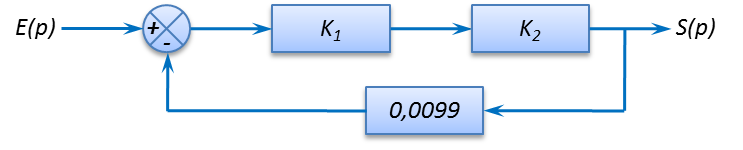
\includegraphics[width=0.7\textwidth]{png/fig_01}\\
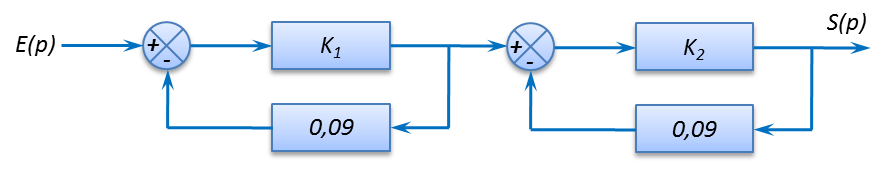
\includegraphics[width=0.7\textwidth]{png/fig_02}
\end{center}


\vspace{.5cm}

Le premier système a pour fonction de transfert $H_1(p)$ et le deuxième $H_2(p)$. 

\subsubsection{Travail demandé}
\begin{enumerate}
\item Calculer $H_1(p)$ et $H_2(p)$.
\item On pose $K_1=K_2=K$. Calculer $K$ tel que $H_1(p)=H_2(p)$.
\end{enumerate}

\correction{
\begin{enumerate}
\item Dans le premier cas, on peut calculer la fonction de transfert en boucle fermée :
$$
H_1(p)=\dfrac{S(p)}{E(p)}=\dfrac{K_1(p)K_2(p)}{1+K_1(p)K_2(p) K_3}
$$

Dans le second cas, deux FTBF se succèdent. On a :
$$
H_2(p)=\dfrac{S(p)}{E(p)}=\dfrac{K_1(p)}{1+K_1(p) K_4}\cdot \dfrac{K_2(p)}{1+K_2(p) K_3}
= \dfrac{K_1(p) K_2(p)}{\left(1+K_1(p)K_4\right)\cdot\left(1+K_2(p)K_4\right)}
$$
\item Dans le premier cas :
$$
H_1(p) = \dfrac{K^2}{1+K^2 K_3}
$$

Dans le second cas :
$$
H_2(p)= \dfrac{K^2}{\left(1+KK_4\right)\cdot\left(1+KK_4\right)}
= \dfrac{K^2}{ 1+K^2K_4^2+2KK_4}
$$

Ainsi,
$$
H_1(p)=H_2(p) 
\Longleftrightarrow 
\dfrac{K^2}{1+K^2 K_3}= \dfrac{K^2}{ 1+K^2K_4^2+2KK_4}
\Longleftrightarrow 
\dfrac{1}{1+K^2 K_3}= \dfrac{1}{ 1+K^2K_4^2+2KK_4}
$$

$$
\Longleftrightarrow 
1+K^2 K_3 = 1+K^2K_4^2+2KK_4
\Longleftrightarrow 
K K_3 = KK_4^2+2K_4
\Longleftrightarrow 
K = \dfrac{2K_4}{K_3-K_4^2} = 100
$$
\end{enumerate}
}
\newpage

%--------------------------------------------

\exercice{Schémas blocs élémentaires}

On considère le système suivant : 
\begin{center}
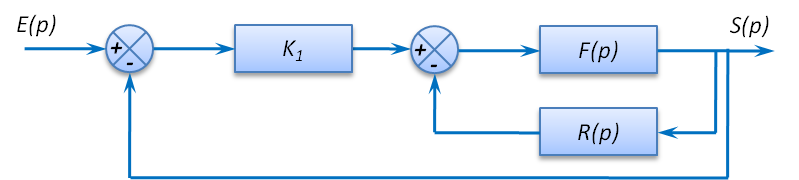
\includegraphics[width=.7\textwidth]{png/fig_03}
\end{center}

\subsubsection{Travail demandé}
\begin{enumerate}
\item Calculer la fonction de transfert $H(p)$ du système.
On donne pour valeur aux différents blocs $F(p)=\dfrac{8}{p\left(p+4 \right)\left( p+5\right)}$, $R(p)=p$ et $K_1 = 5$.
\item Calculer $H(p)$.
\end{enumerate}


\correction{
\begin{enumerate}
\item Schéma bloc équivalent :
\begin{center}
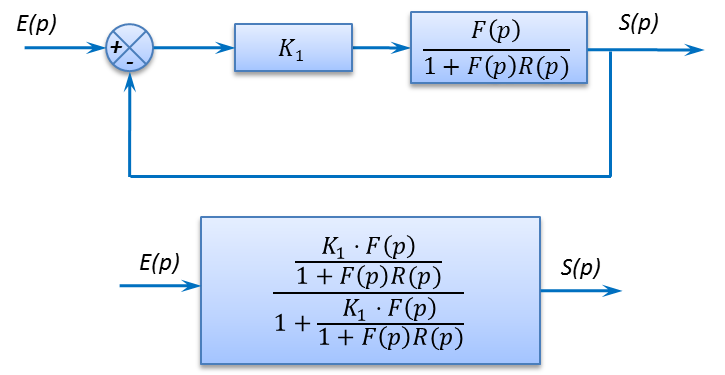
\includegraphics[width=.6\textwidth]{png/fig_03_Corr}
\end{center}

$$
\dfrac{S(p)}{E(p)} = \dfrac{K_1 F(p)}{1+F(p)R(p)+K_1 F(p)}
$$
\item On remplace les fonctions de transfert par leurs valeurs : 
$$
\dfrac{S(p)}{E(p)} = \dfrac{K_1 \dfrac{8}{p\left(p+4 \right)\left( p+5\right)}}{1+\dfrac{8p}{p\left(p+4 \right)\left( p+5\right)}+K_1 \dfrac{8}{p\left(p+4 \right)\left( p+5\right)}}
= \dfrac{8 K_1}{p\left(p+4 \right)\left( p+5\right)+8p+8 K_1 }
$$
\end{enumerate}
}
\newpage

%--------------------------------------------

\exercice{Schémas blocs élémentaires}

Déterminer la sortie $S(p)$ et éventuellement la fonction de transfert correspondant aux schémas suivants : 

\begin{enumerate}
\item Premier système
\begin{center}
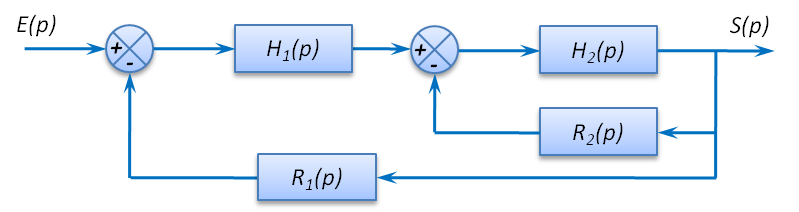
\includegraphics[width=.7\textwidth]{png/fig_04}
\end{center}
\item Deuxième système
\begin{center}
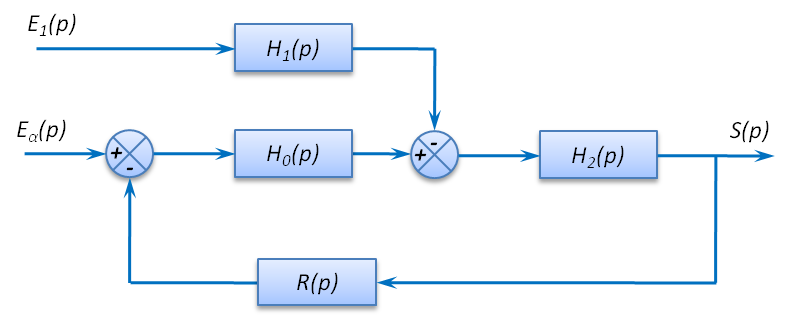
\includegraphics[width=.7\textwidth]{png/fig_05}
\end{center}
\item Troisième système
\begin{center}
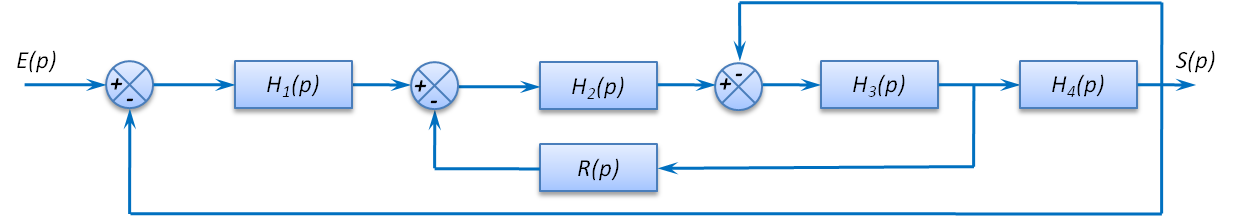
\includegraphics[width=\textwidth]{png/fig_06}
\end{center}
\end{enumerate}

\correction{
\begin{enumerate}
\item Premier système
\begin{center}
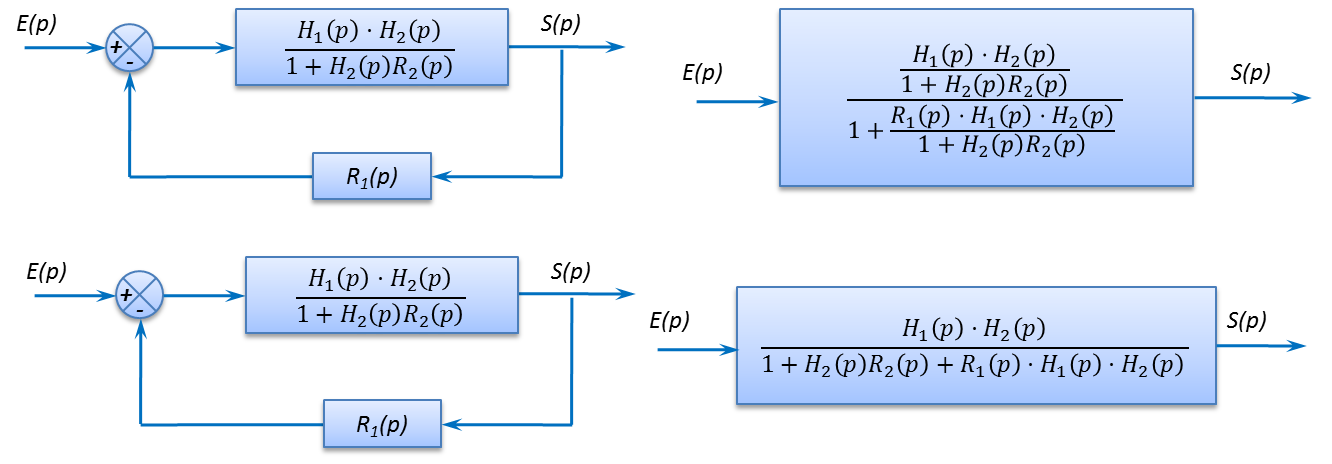
\includegraphics[width=.9\textwidth]{png/fig_04_Corr}
\end{center}
\item Deuxième système\\
On note $G_1(p)=\dfrac{S(p)}{E_\alpha (p)}$ lorsque $E_1(p)=0$ : 
$$
G_1(p)=\dfrac{H_0(p)\cdot H_2(p)}{1+H_0(p)\cdot H_2(p)\cdot R(p)}
$$

On note $G_2(p)=\dfrac{S(p)}{E_1(p)}$ lorsque $E_{\alpha}(p)=0$ :
$$
G_2(p)=-H_1(p)\cdot \dfrac{H_2(p)}{1+H_0(p)\cdot H_2(p)\cdot R(p)}
$$

Au final, 
$$
S(p)=G_1(p)E_{\alpha}(p) + G_2(p) E_1(p)
$$
\item Troisième système
\begin{center}
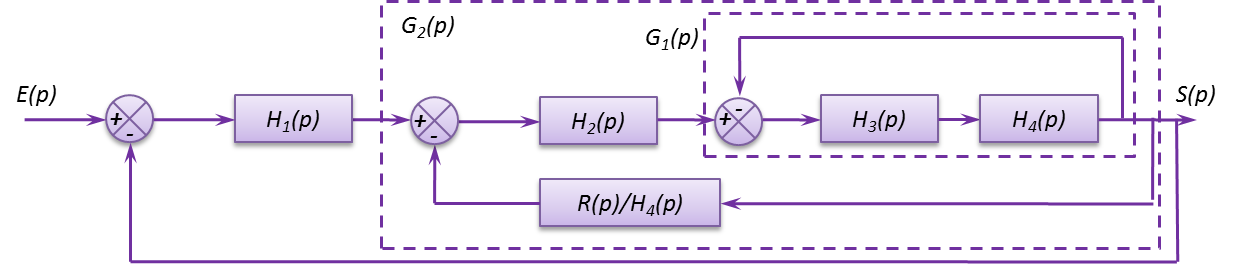
\includegraphics[width=.9\textwidth]{png/fig_06_Corr}
\end{center}
On a :
$$
G_1(p)=\dfrac{H_3(p)\cdot H_4(p)}{1+H_3(p)\cdot H_4(p)}
$$

\begin{align*}
G_2(p) &= 
\dfrac{H_2(p)\cdot G_1(p)}{1+H_2(p)\cdot G_1(p)\cdot\dfrac{R(p)}{H_4(p)}}
= 
\dfrac{H_2(p)\cdot \dfrac{H_3(p)\cdot H_4(p)}{1+H_3(p)\cdot H_4(p)}}{1+H_2(p)\cdot \dfrac{H_3(p)\cdot H_4(p)}{1+H_3(p)\cdot H_4(p)}\cdot\dfrac{R(p)}{H_4(p)}}\\
&= 
\dfrac{H_2(p)\cdot H_3(p)\cdot H_4(p)}{1+H_3(p)\cdot H_4(p)+H_2(p)\cdot H_3(p)\cdot R(p)}
\end{align*}

Au final, 
$$
H(p)=\dfrac{H_1(p)\cdot G_2(p)}{1+H_1(p)\cdot G_2(p)}
=
\dfrac{H_1(p)\cdot \dfrac{H_2(p)\cdot H_3(p)\cdot H_4(p)}{1+H_3(p)\cdot H_4(p)+H_2(p)\cdot H_3(p)\cdot R(p)}}{1+H_1(p)\cdot \dfrac{H_2(p)\cdot H_3(p)\cdot H_4(p)}{1+H_3(p)\cdot H_4(p)+H_2(p)\cdot H_3(p)\cdot R(p)}}
$$
$$
H(p)=
\dfrac{H_1(p)\cdot H_2(p)\cdot H_3(p)\cdot H_4(p)}{1+H_3(p)\cdot H_4(p)+H_2(p)\cdot H_3(p)\cdot R(p)+H_1(p)\cdot H_2(p)\cdot H_3(p)\cdot H_4(p)}
$$
\end{enumerate}
}
\newpage

%--------------------------------------------

\exercice{Schémas blocs élémentaires}
D\'eterminez la fonction de transfert, $H(p)= \frac{S}{E}$, des schémas blocs suivant :
\begin{itemize}
\item Sch\'ema bloc $1$ :
\begin{center}
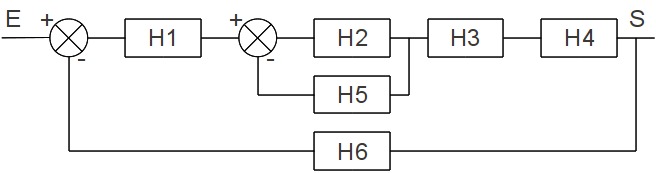
\includegraphics[scale=0.8]{png/schemabloc1.png}
\end{center}
\item Sch\'ema bloc $2$ :
\begin{center}
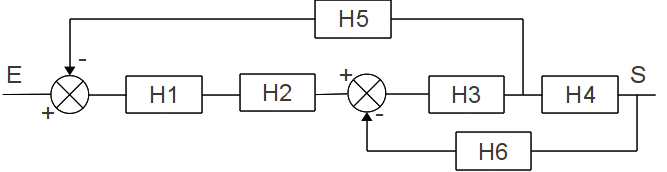
\includegraphics[scale=0.8]{png/schemabloc2.png}
\end{center}
\end{itemize}

\correction{ % Answer
\begin{itemize}
\item Schéma bloc $1$ : \[\frac{S}{E}=\frac{\frac{H_1H_2H_3H_4}{1+H_2H_5}}{1+\frac{H_1H_2H_3H_4H_6}{1+H_2H_5}}\]
\item Schéma bloc $2$ : \[\frac{S}{E}=\frac{H_1H_2H_3H_4}{1+H_3(H_4H_6+H_1H_2H_5)}\]
\end{itemize}
}
\newpage

%--------------------------------------------

\exercice{Système asservi}
D\'eterminez la fonction de transfert, $H(p)= \frac{S(p)}{E(p)}$, du schéma bloc suivant :

\begin{center}
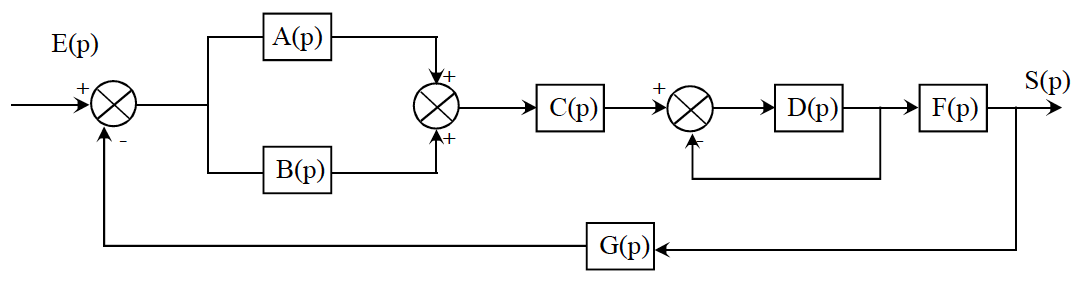
\includegraphics[scale=0.4]{png/SB3.png}
\end{center}

\textit{Remarque : pour alléger l'écriture des calculs, on pourra noter $A$, $B$, $C$\dots les fonctions $A(p)$, $B(p)$, $C(p)$\dots}

\correction{ % Answer
\[\frac{S}{E}=\frac{(A+B).C.D.F}{1+D+(A+B).C.D.F.G}\]
}
\newpage

%--------------------------------------------

\exercice{Moteur à courant continu}
Considérons un moteur à courant continu ayant pour modèle de connaissance les équations suivantes :

\begin{center}
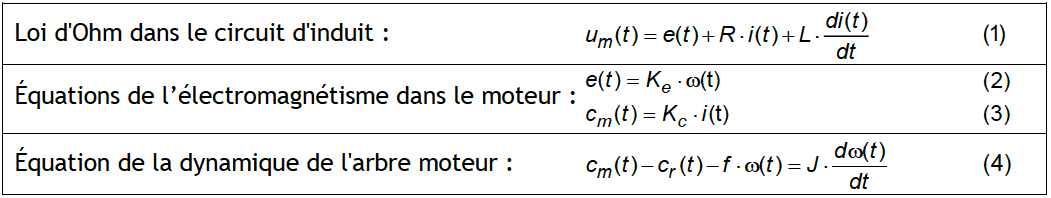
\includegraphics[scale=0.4]{png/MCC_data1.png}
\end{center}

avec :

\begin{center}
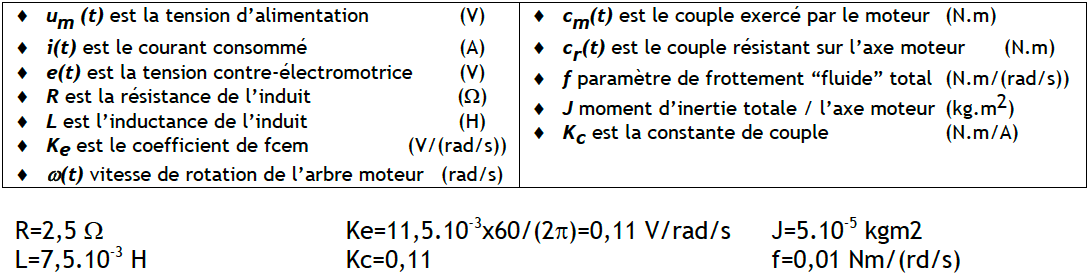
\includegraphics[scale=0.4]{png/MCC_data2.png}
\end{center}

\subsubsection{Travail demandé}
\begin{enumerate}
\item Les conditions initiales étant nulles, compléter le shéma-bloc ci-dessous dans le domaine de Laplace.
\begin{center}
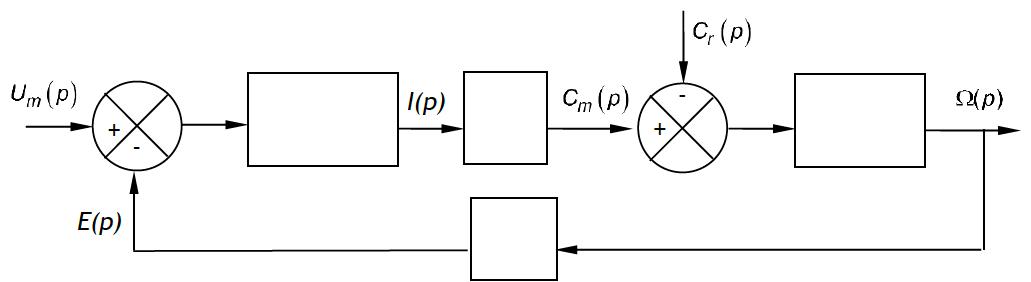
\includegraphics[scale=0.4]{png/MCC_bloc.png}
\end{center}
\item Ce shéma comporte une boucle et des comparateurs. Est-ce un système asservi ?
\item Exprimer de façon littérale la fonction de transfert $\frac{\Omega(p)}{U_m(p)}$ pour $C_r(p)=0$ (sans perturbation).
\item Exprimer de façon littérale la fonction de transfert $\frac{\Omega(p)}{C_r(p)}$ pour $U_m(p)=0$.
\item En précisant le théorème utilisé, en déduire l'expression de $\Omega(p)$ en fonction de $U_m(p)$ et $C_r(p)$.
\item Donner l'expression de $\omega(t=+\infty)$ lorsque $u_m(t)=U_{m0}$ (constante) et $c_r(t)=C_{r0}$ (constante).
\item Vérifier que $K_c.U_{m0}$ et $R.C_{r0}$ sont de même dimension ainsi que $R.f$ et $K_e.K_c$.
\item Faire l'application numérique pour les deux valeurs de $C_{r0}$ ($0$ et $0,3 N.m$) et pour $U_{m0}=10V$.
\item Ces résultats sont-ils cohérents avec la courbe ci-dessous obtenue par simulation numérique ?
\begin{center}
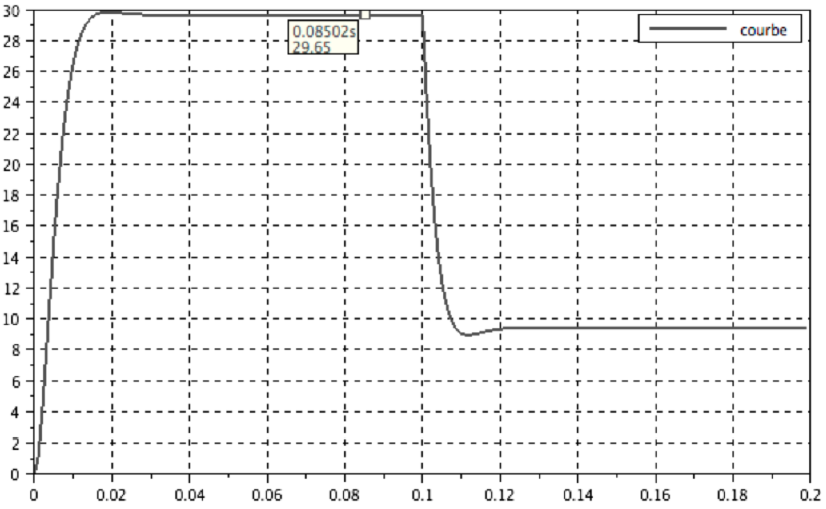
\includegraphics[scale=0.5]{png/MCC_releves.png}
\end{center}
\end{enumerate}

\correction{ % Answer
\begin{enumerate}
\item Schéma bloc :
\begin{center}
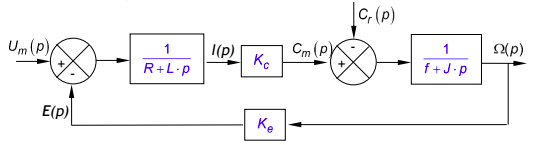
\includegraphics[scale=0.7]{png/MCC_bloc-cor.png}
\end{center}
\item NON. La grandeur de sortie n'est pas de même nature que la grandeur d'entrée. Il n'y a pas de capteur. Le schéma représente la structure des équations différentielles du modèle de connaissances, pas un système asservi.
\item Avec $C_r(p)=0$ :
\[\frac{\Omega(p)}{U_m(p)}=(\frac{K_c}{R.f+K_e.K_c}).(\frac{1}{1+\frac{R.J+L.f}{R.f+K_e.K_c}p+\frac{L.J}{R.f+K_e.K_c}p^2})=F_1(p) \]
\item Avec $U_m(p)=0$ :
\[\frac{\Omega(p)}{U_m(p)}=(\frac{-R}{R.f+K_e.K_c}).(\frac{1+\frac{L}{R}p}{1+\frac{R.J+L.f}{R.f+K_e.K_c}p+\frac{L.J}{R.f+K_e.K_c}p^2})=F_2(p) \]
\item Si $C_r(p)$ et $U_m(p)$ sont non nulles alors : $\Omega(p)=F_1(p)U_m(p)+F_2(p)C_r(p)$ (Théorème de superposition)
\item \[\omega(+\infty)=\lim_{t \leftrightarrow 0}p\Omega(p)=\frac{K_c.U_m{m0}-R.C_{r0}}{R.f+K_e.K_c} \]
\item Cf. dimensions données dans l'énoncé
\item AN : $\omega(+\infty)=29,6 rad/s$ pour $C_{r0}=0$ et  $\omega(+\infty)=9,4 rad/s$ pour $C_{r0}=0,3$.
\item Ces résultats sont similaires à ceux obtenu par simulation. Ce qui est cohérent puisque la simulation ne fait que résoudre numériquement les mêmes équations du modèles de connaissance.
\end{enumerate}
}
\newpage

%--------------------------------------------


%----------------------------------------------------------------------------------------
%	Fonctions de transfert du 1er ordre
%----------------------------------------------------------------------------------------
\section{Fonctions de transfert du 1er ordre}

%--------------------------------------------
\exercice{Identification des systèmes d'ordre 1}

\begin{enumerate}
\item Pour chacune des courbes suivantes, donner l'expression de la fonction de transfert.
\end{enumerate}

\begin{minipage}[c]{.49\linewidth}
\begin{center}
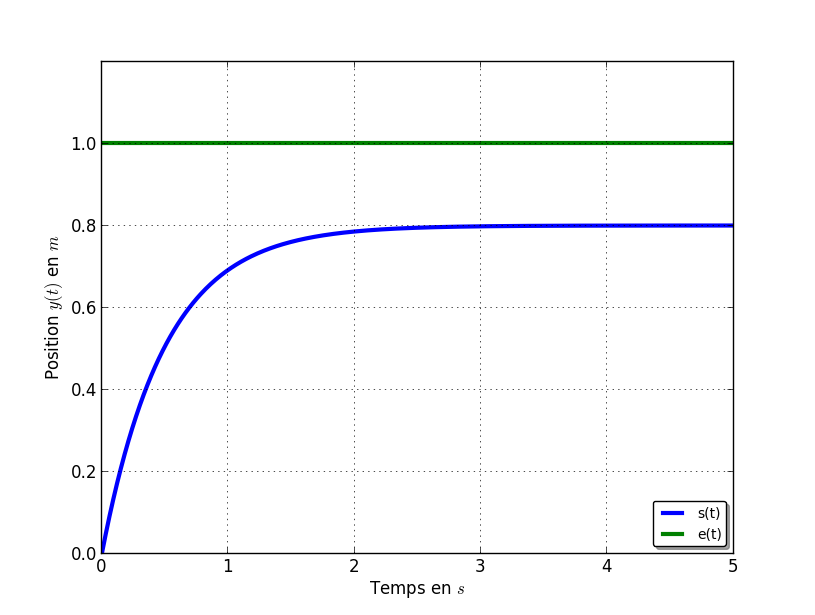
\includegraphics[width=\textwidth]{png/courbe1-1O}
\end{center}
\end{minipage}\hfill
\begin{minipage}[c]{.49\linewidth}
\begin{center}
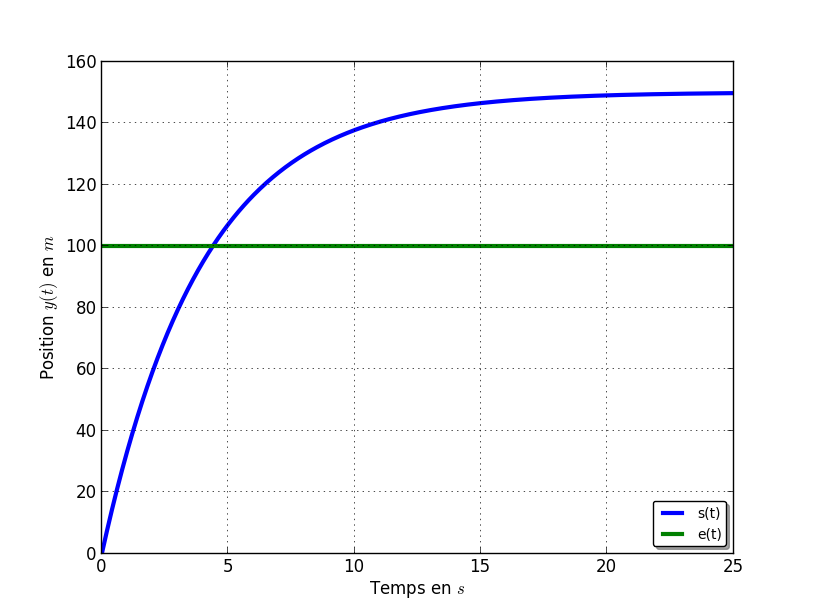
\includegraphics[width=\textwidth]{png/courbe2-1O}
\end{center}
\end{minipage}

\begin{minipage}[c]{.49\linewidth}
\begin{center}
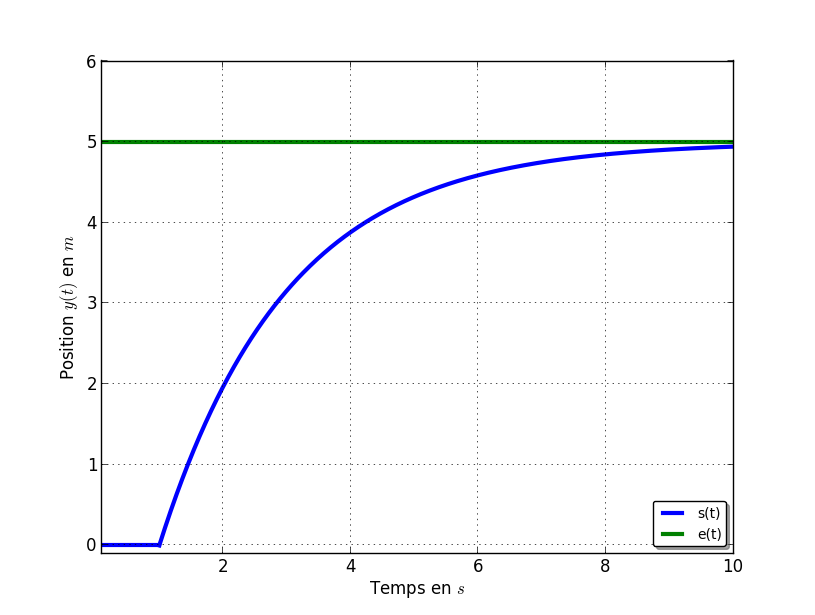
\includegraphics[width=\textwidth]{png/courbe3-1O}
\end{center}
\end{minipage}\hfill
\begin{minipage}[c]{.49\linewidth}
\begin{center}
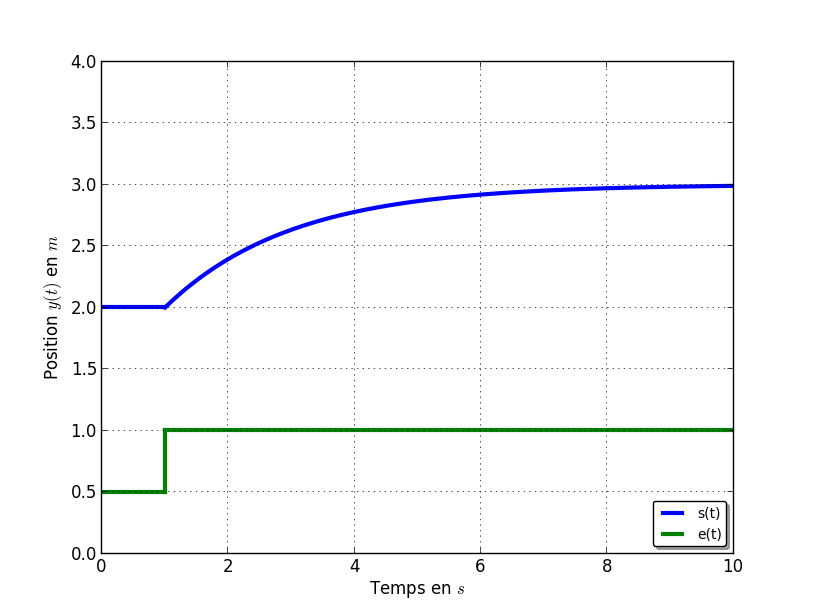
\includegraphics[width=\textwidth]{png/courbe4-1O}
\end{center}
\end{minipage}
\newpage

%--------------------------------------------
\exercice{Étude des performances du système d'ouverture de porte automatique de TGV}
\begin{minipage}[c]{.45\linewidth}
\begin{center}
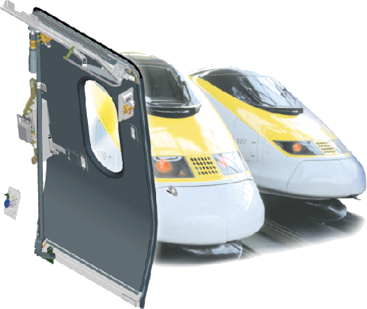
\includegraphics[width=.6\textwidth]{png/fig_01-TGV}
\end{center}
 
 La figure de droite montre l’interface assurant, à partir des informations délivrées par l’unité centrale de commande, la fermeture hermétique et le verrouillage d’une porte de TGV. 
 
\end{minipage} \hfill
\begin{minipage}[c]{.52\linewidth}
\begin{center}
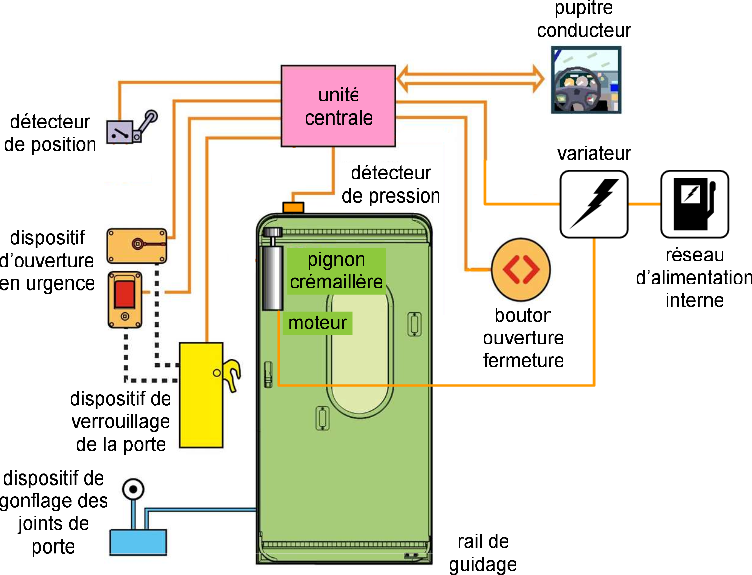
\includegraphics[width=\textwidth]{png/fig_02-TGV}
\end{center}
\end{minipage}

\begin{minipage}[c]{.6\linewidth}
Afin de satisfaire les contraintes d'encombrement, l'ouverture de la porte s'effectue selon l'enchaînement temporel de trois phases distinctes décrites à partir de la position « porte fermée » pour laquelle la face extérieure de la porte est alignée avec la face extérieure de la caisse : une phase de décalage puis une phase de louvoiement et enfin une phase d'escamotage. La phase primaire (décalage) puis la phase terminale (escamotage) sont définies par les figures ci-contre. 

\end{minipage} \hfill
\begin{minipage}[c]{.35\linewidth}
\begin{center}
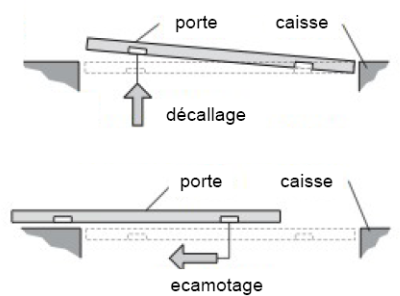
\includegraphics[width=\textwidth]{png/fig_03-TGV}
\end{center}
\end{minipage}

\vspace{0.5cm}
Les performances annoncées de la part du constructeur, dans la phase d'escamotage, sont les suivantes :
\vspace{0.5cm}
\begin{center}
\begin{tabular}{|l|l|}
\hline
Critères & Valeur \\
\hline
\hline
Accès suffisant du wagon & 850 mm \\
\hline
Temps d'ouverture de la porte en phase d'escamotage & $t\leq 4\; s$ \\
\hline
Vitesse d’accostage de la porte en fin de phase d’escamotage & $V\leq 0,09 \; m/s$ \\
\hline
\end{tabular}
\end{center}
\vspace{0.5cm}

Pour ouvrir la porte, on utilise un moteur, dont la rotation est transformée en translation par l'intermédiaire d'un système pignon crémaillère. La translation de la porte est notée $y(t)$. L'angle de rotation du moteur est noté $\theta_m(t)$. Le lien entre $y(t)$ et $\theta_m (t)$ est $y(t) = R\cdot\theta_m (t)$ où $R$ est le rayon du pignon ($R=37\; mm$).

On fait l'hypothèse qu'à l'instant initial, correspondant au début de la translation de la porte, la porte est immobile, avec $y(t=0)=0$ et $\theta_m (t=0)=0$ (toutes les autres conditions initiales seront également nulles, par conséquent).

Grâce à une redéfinition du paramétrage et dans un souci de simplification, on considère qu'au cours de cette d phase la vitesse angulaire du moteur vérifie $\omega_m (t) = \dot{\theta}_m (t) \geq 0$ et la position de la porte vérifie $y(t) \geq 0$.  


On donne le modèle de connaissance du moteur courant continu du système :
$$u_m(t) = e(t) + R\cdot i(t) 
\quad e(t) = k\cdot \omega_m(t) 
\quad J\cdot \dfrac{d\omega_m(t)}{dt} = C_m (t)
\quad C_m (t) = k_m \cdot i(t)$$

\vspace{0.5cm}
Avec : 
\begin{itemize}
\item $u_m (t)$ : tension du moteur; 
\item $e(t)$ : force contre électromotrice du moteur; 
\item $i(t)$ :intensité dans le moteur;
\item $C_m (t)$ : couple exercé par le moteur;
\item $\omega_m(t)$ : vitesse angulaire du moteur.
\end{itemize}

\subsubsection{Travail demandé}
\begin{enumerate}
\item Exprimer ces équations dans le domaine de Laplace.
\item Schématiser le schéma-bloc du moteur en s’aidant des équations de la question 1.
\item Montrer que, dans le domaine de Laplace, la relation entre $\Omega_m (p)$ et $U_m (p)$ peut s'écrire sous la forme : $\dfrac{\Omega_m(p)}{U_m(p)} = \dfrac{K}{1+Tp} $ où $K$ et $T$ sont deux constantes à déterminer.
\item Déterminer $\omega_m (t)$ lorsque le moteur est soumis à un échelon de tension d'amplitude $u_0$ tel que : $u_m (t)= u_0 \cdot u(t)$. Exprimer et justifier le résultat en fonction de $K$ et $T$.
\item L'application numérique fournit $K=1,2 \; s^{-1}\cdot V^{-1}$ et $T=0,16\;s$. Déterminer le temps de réponse à 5\% du moteur.\\
Le schéma bloc du système peut se mettre sous la forme suivante :
\begin{center}
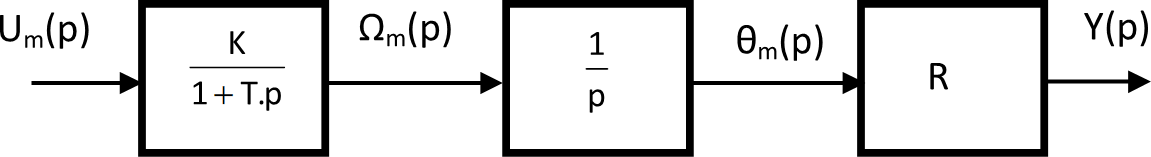
\includegraphics[width=.5\textwidth]{png/fig_04-TGV}
\end{center} 
\item Justifier la fonction de transfert entre $\Omega_m(p)$ et $\theta_m (p)$.
\item Déterminer l'expression analytique de $\dfrac{Y(p)}{U_m(p)}$.
\item Déterminer l'expression analytique de $y(t)$ lorsque le moteur est soumis à un échelon de tension d'amplitude $u_0$.
\item Déterminer la valeur numérique du déplacement de la porte au bout de 4s ($u_0 =5V$), et conclure quant à la capacité du système à satisfaire le critère d'accès au wagon du cahier des charges.
\item Déterminer la vitesse de la porte à la fin de la translation ($v(t=4s)= \dfrac{d}{dt}y(t=4s)$). Conclure quant à la capacité du système à satisfaire le critère de vitesse finale de translation de la porte du cahier des charges.
\end{enumerate}
\newpage

%--------------------------------------------
\exercice{Robot de manutention}

\subsubsection{Présentation}

Dans ce qui suivra on se placera dans l’hypothèse de systèmes linéaires continus et invariants.


\begin{minipage}[c]{.3\linewidth}
\begin{center}
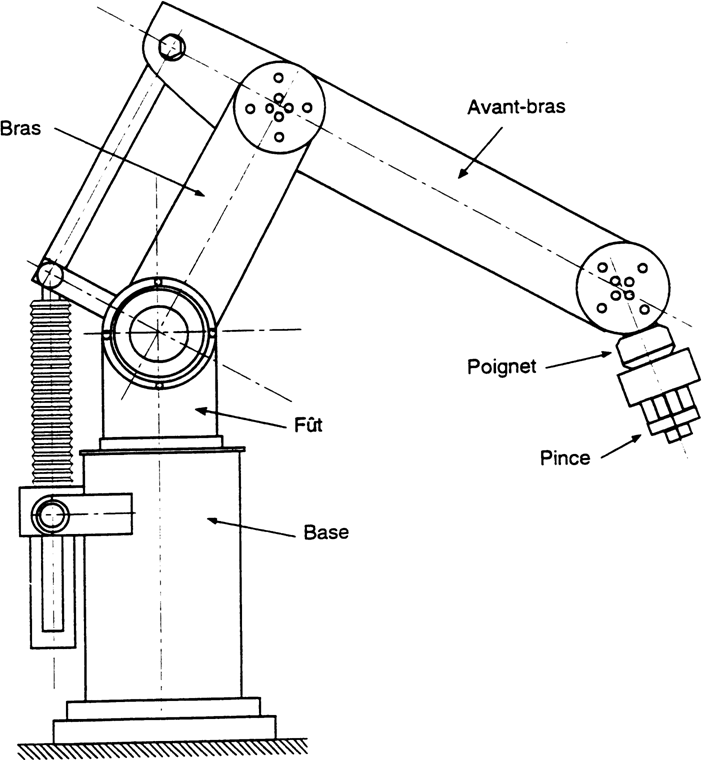
\includegraphics[width=\textwidth]{png/fig_01-1O}
\end{center}
\end{minipage} \hfill
\begin{minipage}[c]{.65\linewidth}
Principales notations utilisées : 
\begin{itemize}
\item $J_m$ : inertie du moteur, du réducteur et de la charge;
\item $J_{me}$ : inertie globale équivalente sur l’arbre moteur;
\item $C_m$ : couple électromagnétique délivré par le moteur;
\item $C_{re}$ : couple résistant ramené sur l’arbre moteur ou couple équivalent;
\item $R$, $Ke$, $Kt$ : constantes électriques du moteur (résistance de l’induit, constante 	de force contre électromotrice et constante de couple);
\item $N$ : rapport de réduction;
\item $\omega_m$, $\theta_m$ : vitesse et position angulaire du moteur;
\item $\omega_c$, $\theta_c$ : vitesse et position angulaire de la charge.
\end{itemize}
\end{minipage}

On se propose tout d’abord d’étudier le modèle du moteur à vide c’est à dire du moteur seul : dans un premier temps par un modèle théorique et dans un second temps par une étude expérimentale. Ensuite il sera fait mention de la charge puis de la réalisation de l’asservissement de position.

\subsubsection{Étude théorique du moteur seul}

Le moteur retenu pour animer la rotation du fût par rapport à la base est un servomoteur PARVEX de type AXEM à induit plat qui présente l’avantage de posséder une très faible inertie. C’est un moteur à courant continu.

Le comportement électromécanique de ce moteur dans l’hypothèse où l’inductance est négligeable, est donné par les équations suivantes :

\begin{eqnarray*}
u(t)=Ri(t)+e(t) \\
C_m(t)=K_t i(t) \\
e(t)= K_e \omega_m(t) \\
J_m \dfrac{d\omega_m (t)}{dt} = C_m(t)
\end{eqnarray*}


\begin{enumerate}
\item En faisant l’hypothèse de conditions initiales sont nulles, calculez la transformée de Laplace $\Omega(m)$ en fonction de la transformée de Laplace $U(p)$.
\item Mettez le résultat sous la forme $\Omega_m(p)=\dfrac{K_m}{1+T_m p} U_m(p)$ en précisant $K_m$ et $T_m$.
\item Les données du constructeur permettent de connaître les valeurs suivantes : $K_e=25,5\; V/(1000\; tr/min))$, $K_t=0,244 \; Nm/A$, $R=0,46\, \Omega$.\\
Faites un calcul approché permettant de déterminer $K_m$ et $T_m$ ($T_m$  sera fonction de $J_m$  pour l’instant non connu).\\
\textit{Remarque : pour toutes les applications numériques utilisez des unités S.I.}
\end{enumerate}

\subsubsection{Étude pratique du moteur seul}

Afin de valider le modèle précédent et de déterminer l’inertie du rotor du moteur on effectue une étude expérimentale sous la forme de l’observation de la réponse du moteur seul soumis à un échelon de tension de 50 V. Le résultat de cet essai est donné sur la courbe suivante.

\begin{center}
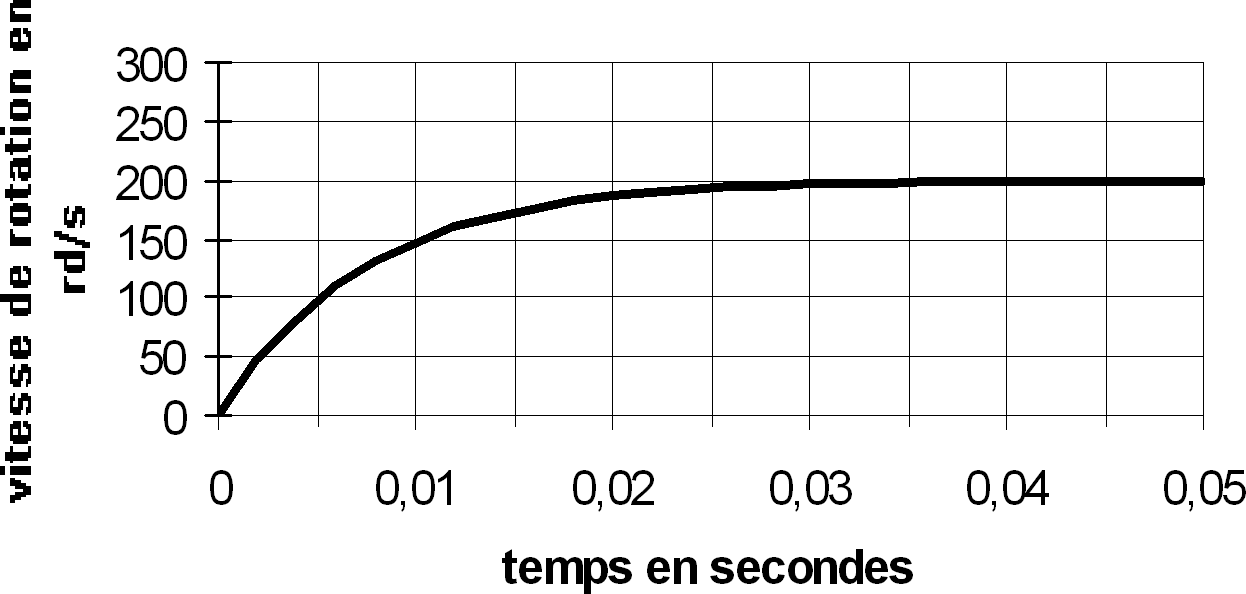
\includegraphics[width=.5\textwidth]{png/fig_02-1O}
\end{center}

\begin{enumerate}
\item Cette courbe est-elle bien conforme au modèle du premier ordre de la question précédente ? Pourquoi ?
\item Déterminez les valeurs expérimentales de $K_m$ et $T_m$. Déduisez-en la valeur expérimentale de $J_m$.
\end{enumerate}

\subsubsection{Motorisation complète avec réducteur et charge}

La charge que devra entraîner le moteur est maintenant prise en compte ainsi que le réducteur qui permet de réduire la vitesse $\omega_m$ de rotation du moteur. En sortie du réducteur la vitesse de rotation est $\omega_c$.

L’inertie du moteur seule $J_m$ devient $J_{me}$ inertie équivalente de l’ensemble  charge + moteur + réducteur.

La charge crée un couple résistant équivalent $C_{re}$. On obtient donc l’équation suivante :
$$
C_m(t)=J_{me}\dfrac{d\omega_m(t)}{dt} + C_{re}(t)
$$

\begin{enumerate}
\item A partir des équations électriques du moteur et de l’équation précédente, exprimez la transformée $\Omega_m(p)$. Les dénominateurs seront mis sous la forme $(1+T_{me} p)$. On précisera l’expression de $T_{me}$.
\item A partir du résultat précédent complétez le schéma fonctionnel suivant et explicitez clairement $G_1$, $G_2$, $G_3$, $G_4$. $G_3$ sera exprimé sous la forme d’un premier ordre avec pour constante de temps $T_{me}$.
\end{enumerate}

\begin{center}
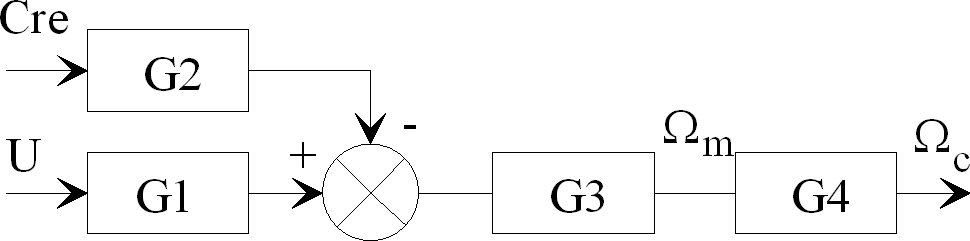
\includegraphics[width=0.5\textwidth]{png/fig_03-1O}
\end{center}

\subsubsection{Asservissement de position}

Pour la suite on suppose $C_{re}(p)$  nul. 

 Pour assurer l’asservissement de position angulaire du fût du robot (la sortie est alors un angle exprimé en radian), on associe au moteur un variateur de gain pur $K_a$ placé avant $G_1$ et on met en place un capteur de position angulaire de gain unitaire. Le capteur prendra l’information de position après le réducteur.
 
\begin{enumerate}
\item Faites le schéma fonctionnel de l’asservissement ainsi constitué.
\item Calculez sa fonction de transfert. Donnez-en une interprétation pratique.
\end{enumerate}
\newpage

%----------------------------------------------------------------------------------------
%	Fonctions de transfert du 2ème ordre
%----------------------------------------------------------------------------------------
\section{Fonctions de transfert du 2ème ordre}

%--------------------------------------------
\exercice{Correcteur de phare}
\textit{(Selon le concours CCP PSI 2003)}

\subsubsection{Présentation du système}

L‘assiette d‘un véhicule se modifie avec sa charge, le profil de la route ou les
conditions de conduite (phase de freinage ou d‘accélération). Cette modification
entraîne une variation d‘inclinaison de l‘axe du faisceau lumineux produit par
les phares du véhicule. Ceux ci peuvent alors éblouir d‘autres conducteurs ou
mal éclairer la chaussée.


\begin{center}
 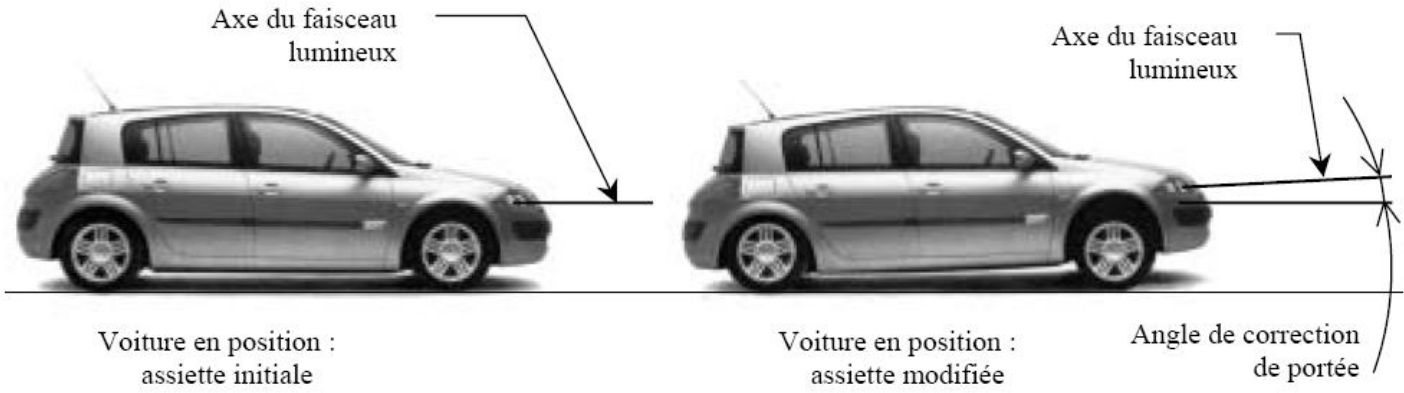
\includegraphics[width=.6\textwidth]{png/image1}
\end{center}
     
         Certaines voitures sont équipées de système de correction de portée. Ce
système fait appel à
des capteurs d‘assiette reliés aux essieux avant et arrière du véhicule. Les
données sont traitées
électroniquement par un calculateur et transmises aux actionneurs situés
derrière les projecteurs. La
position du projecteur est ajustée en maintenant un angle de faisceau optimal
évitant tout
éblouissement et fournissant le meilleur éclairage de la route.
Le système étudié est un correcteur de portée statique, qui corrige la portée
lorsque le véhicule est à
l‘arrêt et conserve cette correction lorsque le véhicule roule (le correcteur ne
tient compte que de la
variation d‘assiette due à la charge).

       Le but de l‘étude est d‘analyser le système et de montrer s‘il est
capable de corriger la portée
de manière dynamique, c‘est à dire en tenant compte des variations d‘assiette
dues au profil de la
route.

\subsubsection{Éléments constitutifs du correcteur de portée}

\textbf{Capteurs d’assiette} : codeurs optiques permettant de mesurer le
débattement des suspensions.

\textbf{Système d’orientation : bloc d’orientation + moto-réducteur + système
vis écrou}

Le bloc d‘orientation supporte les différentes lampes du phare (codes,
clignotants...). Il peut pivoter
par rapport au support lié à la carrosserie autour d‘un axe horizontal (axe de
rotation indiqué sur la
figure ci-dessous). Le bloc est protégé par une vitre liée à la carrosserie. Ce
mouvement est motorisé
grâce au moto-réducteur + système vis écrou. Il existe aussi une possibilité de
réglage manuel en
sortie d‘usine ou en cas de défaillance du système électrique.

\begin{center}
 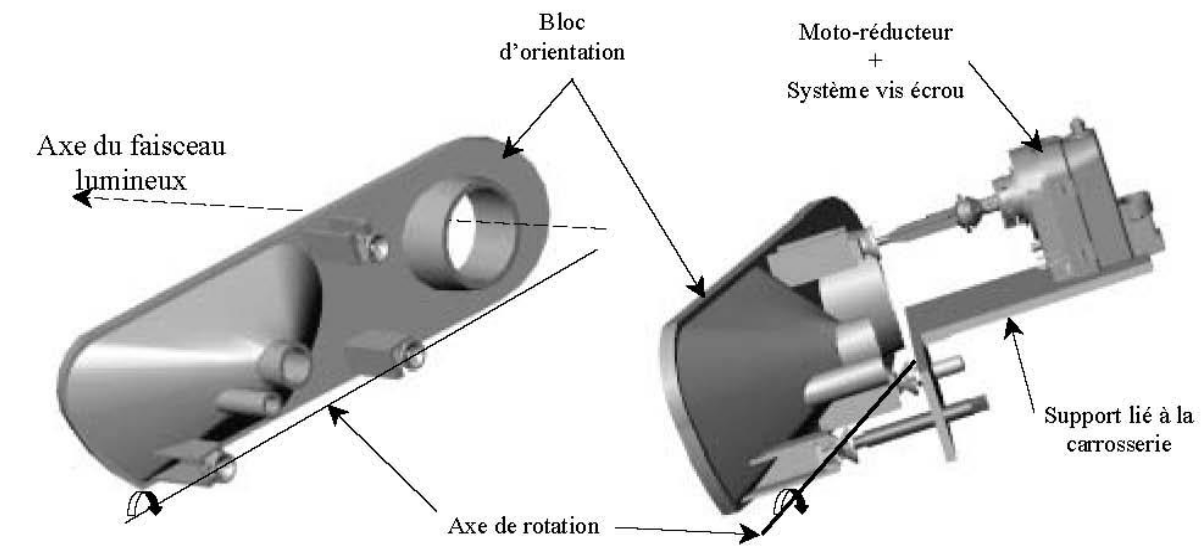
\includegraphics[width=.6\textwidth]{png/image2}
\end{center}

\subsubsection{Diagrammes SADT niveau A-0, A0 et A3}
\begin{center}
 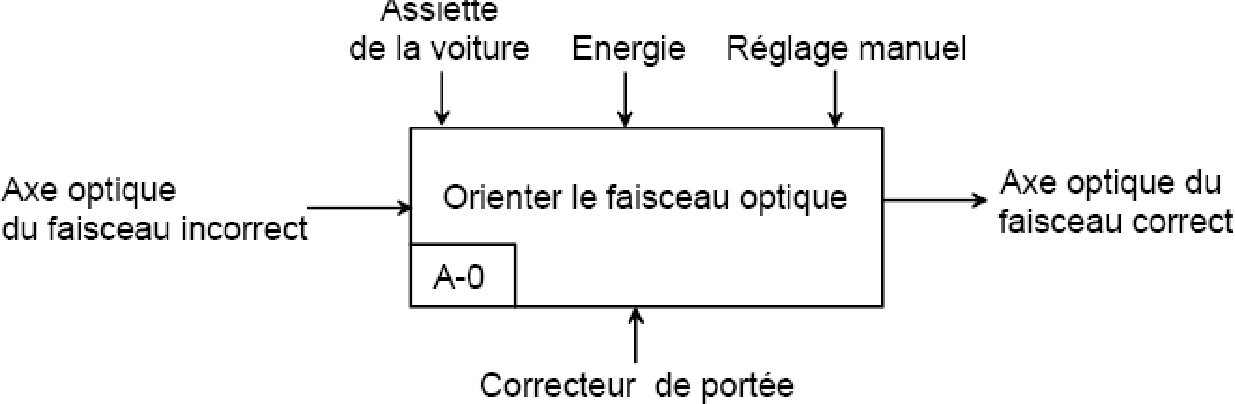
\includegraphics[width=.6\textwidth]{png/image3}
\end{center}

\subsubsection{Étude de la chaîne d’action complète}
La chaîne d‘action complète comprend :
\begin{itemize}
 \item l‘ensemble transducteur (\textbf{capteur + amplificateur + calculateur})
qui mesure l‘angle de tangage $\beta$ du véhicule et commande le moteur du
système. L‘ensemble est assimilable à un gain pur : $K_c$;
\item le \textbf{moteur à courant continu} dont la fonction de transfert est
notée $M(p)$;
\item on équipe ce moteur d‘un retour tachymétrique assimilable à un gain pur : 
   $K_{tachy}=0,03 V.rad^{-1}.s$;
\item le \textbf{réducteur de vitesse} dont le rapport de réduction est de 490;
\item l’ensemble \textbf{vis-écrou} (de pas $p = 6mm$) qui transforme la
rotation de l’axe du réducteur en translation de l’axe de sortie. (NB : 1
tour de la vis fait avancer de 1 pas l’écrou);
\item le \textbf{bloc d‘orientation} : l‘angle de correction de portée
$\theta(t)$ étant petit, on peut linéariser la loi entrée-sortie sur le
domaine d‘utilisation ; l‘angle $\theta(t)$ est proportionnel au déplacement
$x(t)$ de la vis.
\end{itemize}

($\theta(t)$ varie entre $\dfrac{-\pi}{20}$ $\dfrac{\pi}{20}$ et pour
$x(t)$ compris entre -15mm et +15mm).

\begin{enumerate}

\item Refaire, sur votre copie, le diagramme fonctionnel de la chaîne d‘action
ci-dessous, en précisant le nom des constituants dans les blocs, les
informations véhiculées entre les blocs ainsi que leur symbole et leur unité
(les fonctions de transfert ne seront pas déterminées).\\
NB : 
\begin{itemize}
 \item l’entrée $B(p)$ est la transformée de Laplace de $\beta(t)$ et la sortie
$\Theta(p)$, la transformée de Laplace de $\theta(t)$;
\item attention, un bloc modélise le passage de la vitesse angulaire $\Omega(p)$
à la position angulaire $\Theta(p)$.
\end{itemize}

\begin{center}
 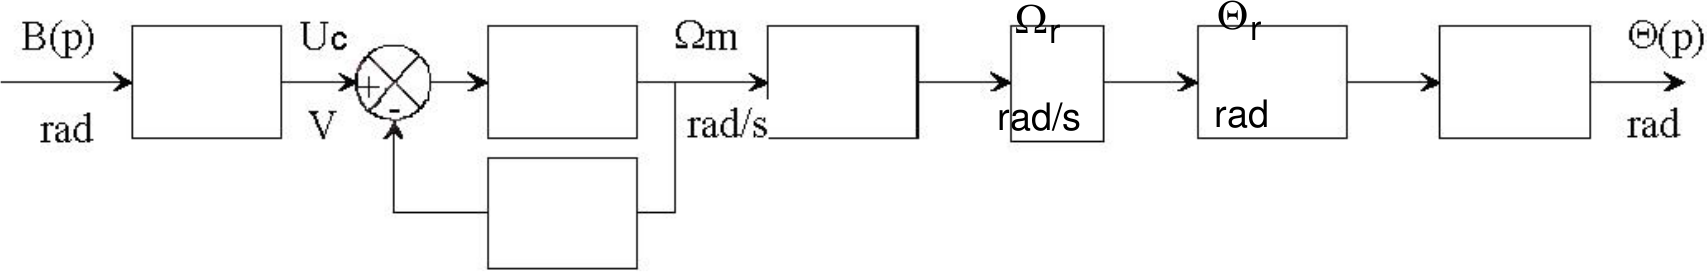
\includegraphics[width=.6\textwidth]{png/image4}
\end{center}

\item Refaire, sur votre copie, le diagramme fonctionnel de la chaîne d‘action
ci-dessus, mais cette fois-ci en précisant les fonctions de transfert de chaque\\
bloc.

Pour déterminer la fonction de transfert du moteur, $M(p)$, on dispose de sa
réponse indicielle (entrée unitaire) :

\begin{center}
 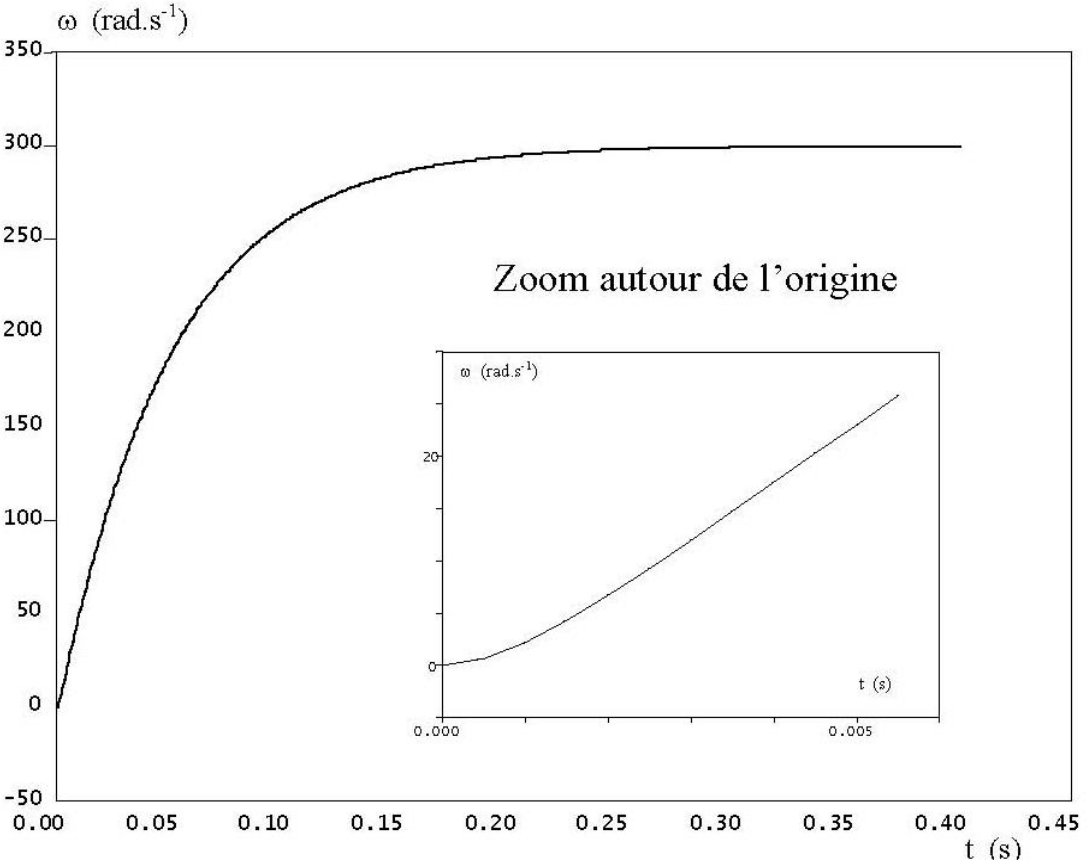
\includegraphics[width=.6\textwidth]{png/image5}
\end{center}


\item Quelle est la forme de la fonction de transfert du moteur et pourquoi ?

\item Quelle hypothèse pouvons-nous faire pour modéliser le système par un
système du 1\up{er}
ordre ?
NB : Pour démontrer ce raisonnement, déterminer la réponse temporelle d’un
système
du 2\up{ème} ordre apériodique, puis simplifier cette réponse avec votre
hypothèse et enfin
conclure.
Cette hypothèse vous semble-t-elle justifiée ici au vu de la réponse indicielle.


\item Identifier $M(p)$ à un 1\up{er} ordre. (Pour cela déterminer les
paramètres caractéristiques sur la courbe).


\item En déduire la fonction de transfert $M'(p)=\dfrac{\Omega_m(p)}{U_c(p)}$
du moteur équipé du retour                                                 
tachymétrique. Quels sont les avantages et les inconvénients de cette boucle de
retour ?\\

La fonction de transfert de la chaîne d‘action complète est donnée
approximativement par :
$H(p)=\dfrac{\Theta(p)}{B(p)}=K_c\dfrac{0,003}{\left(1+0,025p \right)p}$    
(Les angles d‘entrée et de sortie sont exprimés en radian).

Le véhicule est brusquement chargé à l‘arrière.


\item Tracer, SANS FAIRE DE CALCUL, l‘allure de la loi d‘entrée, puis l‘allure
de la réponse.
Justifier votre tracé. Est-ce satisfaisant ?\\


Pour remédier à ce problème on asservit le système en position en plaçant :
\begin{itemize}
 \item un capteur de position, de gain $K_{pos}$ , qui mesure l‘angle $\theta$,
\item un amplificateur de gain pur $A$.
\end{itemize}

\begin{center}
 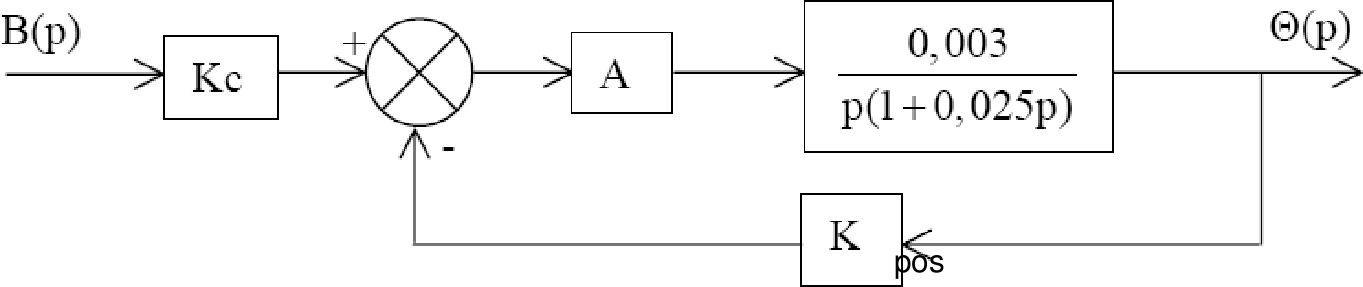
\includegraphics[width=.6\textwidth]{png/image6}
\end{center}


\item Déterminer la nouvelle fonction de transfert $\dfrac{\Theta(p)}{B(p)}$
ainsi que ses paramètres caractéristiques.


\item Expliquer en deux lignes pourquoi le problème a été remédié.

\item À partir de la courbe ci-contre, déterminer la quantité $AK_{pos}$ qui
permet d‘avoir le système le plus rapide. Calculer alors le temps de réponse à
5\% du système.

\begin{center}
 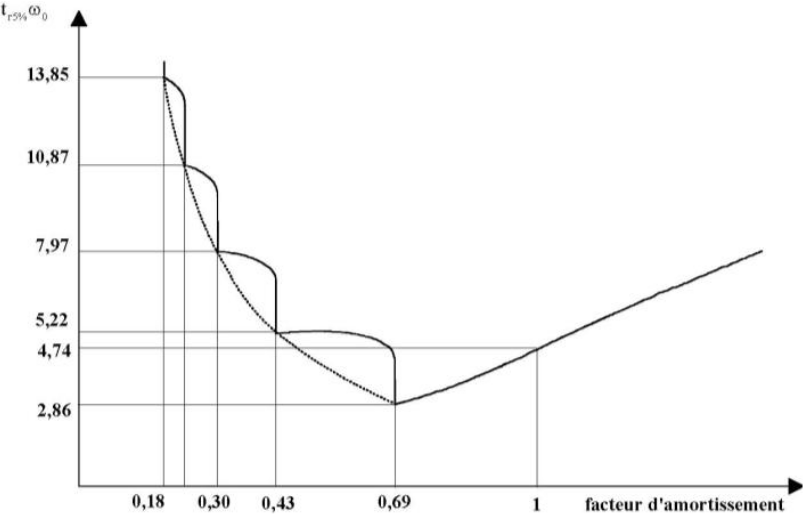
\includegraphics[width=.6\textwidth]{png/image7}
\end{center}
\end{enumerate}
\newpage

%--------------------------------------------

\exercice{Unité dentaire}
\textit{(Selon le concours E3A PSI 2007)}
\vspace{0.25cm}


\begin{minipage}[c]{.6\linewidth}
Le support de l'étude est une "unité dentaire" dont on donne un extrait du cahier des charges fonctionnel. Cet équipement a été conçu et réalisé dans le but d'une adaptabilité maximale aux différentes méthodes de travail des chirurgiens dentistes. Son ergonomie, sa maniabilité, son design, sa fiabilité en font une "unité universelle". Sa conception est modulaire avec une technologie avancée.

Le chirurgien dentiste possède une pédale et un pupitre de commande, qui lui permet de monter ou descendre verticalement le corps du patient, de l'incliner plus ou moins, et de positionner sa tête. Le patient pouvant prendre une position spatiale pertinente, tous les actes médicaux sont facilités.
\end{minipage}\hfill
\begin{minipage}[c]{.35\linewidth}
\begin{center}
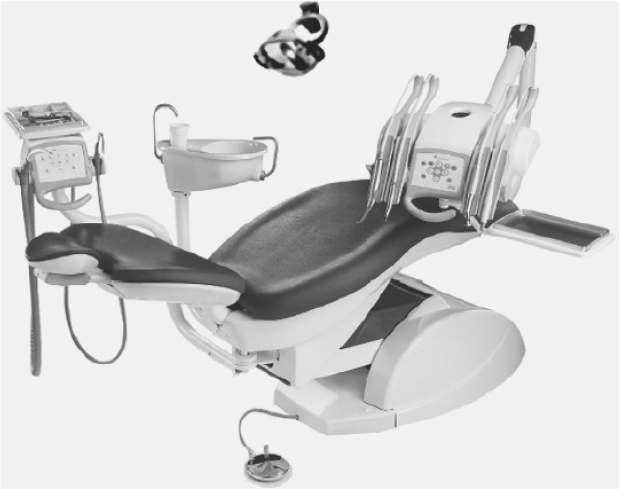
\includegraphics[width=.9\textwidth]{png/fig1-dentaire}
\end{center}
\end{minipage}

\begin{center}
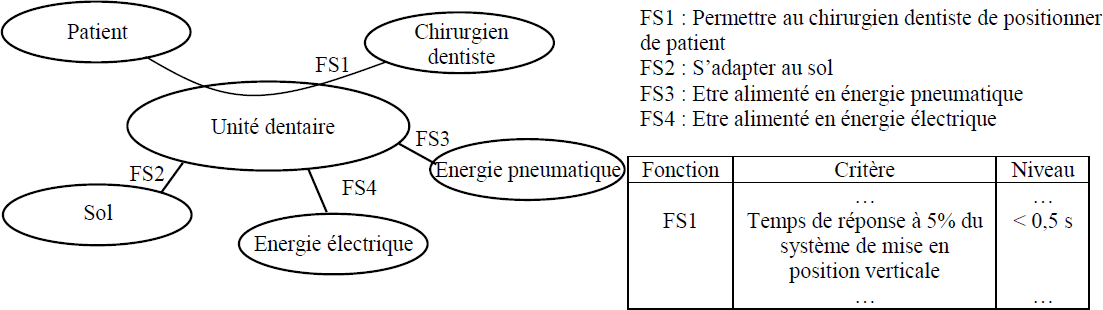
\includegraphics[width=.9\textwidth]{png/fig2-dentaire}
\end{center}

On s'intéresse dans ce sujet au critère de la FS1 concernant le temps de réponse du système permettant de mettre en position verticale le patient. 

Pour régler le patient en position verticale, le chirurgien dentiste appuie sur une pédale, plus ou moins fort. Un moteur électrique se met en route, sa vitesse de rotation dépend de l'appui plus ou moins profond du chirurgien dentiste sur la pédale. La vitesse de rotation du moteur est diminuée par un réducteur à engrenages. En sortie du réducteur à engrenages se trouve une vis dont la rotation $\Omega_v(p)$ entraîne, par un système vis-écrou, la translation du siège en hauteur. L'ensemble peut se représenter par le schéma bloc suivant. Le composant de fonction de transfert $C(p)$ est un correcteur :


\begin{center}
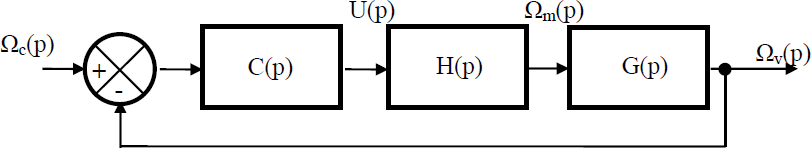
\includegraphics[width=.6\textwidth]{png/fig3-dentaire}
\end{center}

\subsubsection{Travail demandé}
\begin{enumerate}

\item Déterminer le nom des composants qui réalisent les fonctions $H(p)$ et $G(p)$.

\item Déterminer la fonction de transfert en boucle fermée du système $\dfrac{\Omega_v(p)}{\Omega_c(p)}$.\\

Les équations du moteur utilisé sont les suivantes :
$$
u(t)=e(t)+Ri(t)+L\dfrac{di(t)}{dt} \quad e(t) = k_e \omega_m(t) \quad J\cdot\dfrac{d\omega_m(t)}{dt} = C_m(t)-f\omega_m(t) \quad C_m(t)=k_m \cdot i(t)
$$

On note $u(t)$ tension du moteur, $e(t)$, la force contre électro motrice du moteur, $i(t)$ l'intensité dans le moteur, $C_m(t)$ le couple exercé par le moteur et $\omega_m(t)$ la vitesse angulaire du moteur. Les grandeurs physiques $R$, $L$, $k_e$, $J$, $f$ et $k_m$ sont des constantes.

\item En supposant les conditions initiales nulles, exprimer ces équations dans le domaine de Laplace.

\item Montrer que, dans le domaine de Laplace, la relation entre $\Omega_m(p)$ et $U(p)$ peut s'écrire sous la forme d'une fonction de transfert du second ordre. On déterminera les différentes constantes.\\

Si on utilise un correcteur proportionnel, l'application numérique des grandeurs physiques permet de trouver la fonction suivante : $\dfrac{\Omega_v(p)}{\Omega_c(p)} =\dfrac{K_T}{1+T_T p}$ avec $K_T=0,9$ et $T_T=0,1 s.$.

\item Déterminer $\omega_v(t)$ lorsque le chirurgien dentiste demande un échelon de rotation $\omega_c(t)=\omega_{c0}\cdot u(t)$. Exprimer le résultat en fonction de $\omega_{C0}$, $K_T$ et $T_T$.

\item Déterminer le temps de réponse à 5\% du système et effectuer l'application numérique. Conclure vis-à-vis du cahier des charges.\\

Le patient, initialement immobile, bouge verticalement selon le déplacement $x_v(t)$ tel que $\dfrac{dx_v(t)}{dt} = a\omega_v(t)$ avec $a$ constante qui représente le pas réduit de la vis. 

\item Déterminer la transformée de Laplace $X_v(p)$ de $x_v(t)$.

\item Déterminer $x_v(t)$ en fonction de $a$, $K_T$, $T_T$ et $\omega_{c0}$.\\


Si on utilise un correcteur proportionnel, dérivé et intégral, l'application numérique des grandeurs physiques permet de trouver la fonction suivante : $\dfrac{\Omega_v(p)}{\Omega_c(p)} = \dfrac{1}{1+2p+p^2}
$

\item Déterminer $\omega_v(t)$ lorsque le chirurgien dentiste demande un échelon de rotation $\omega_c(t)=\omega_{c0}\cdot u(t)$.

\item Déterminer si le temps de réponse à 5\% est plus faible  ou plus grand que dans le cas précédent. Conclure vis-à-vis du cahier des charges.
\end{enumerate}
\newpage

%----------------------------------------------------------------------------------------
%	Études féquentielles
%----------------------------------------------------------------------------------------
\section{Études fréquentielles}

%--------------------------------------------

\exercice{Tracé \& interprétation d'un diagramme de Bode}
On se propose de d\'eterminer le comportement fr\'equentiel d'un syst\`eme dont la fonction de transfert est donn\'ee :
\begin{description}
\item \[H(p)=\frac{10}{(1+0,003.p+0,25.p^2).(1+0,1.p)}\]
\end{description}
\begin{enumerate}
\item Proposer une m\'ethode pour tracer le diagramme de Bode, en gain et phase, de la fonction de transfert $H(p)$.
\item \'Ecrire les fonctions de transfert isochrones de $H_1(p)$ et $H_2(p)$.
\item Tracer les diagrammes asymptotiques, puis r\'eels, de chacune des fonctions $H_1(j\omega)$ et $H_2(j\omega)$.
\item En d\'eduire le diagramme asymptotique puis réel de $H(j\omega)$.
\item On sollicite le syst\`eme avec les entr\'ees sinuso\"idales :
\begin{itemize}
\item $e_1(t)=3.\sin(1,2.t)$
\item $e_2(t)=3.\sin(120.t)$
\end{itemize}
Donner pour chacune des entr\'ees la r\'eponse en r\'egime permanent.
\end{enumerate}

\correction{ % Answer
\begin{enumerate}
\item On pose $H(p)=H_1(p)H_2(p)$ tel que $H_1(p)$ et $H_2(p)$ soient des fonctions de transfert élémentaires du première ordre ou du deuxième ordre.
\item \[H_1(p)=\frac{1}{1+0,003p+0,25p^2} \mbox{ et } H_2(p)=\frac{10}{1+0,1p}\]\\
\textit{Remarque : On obtient les fonctions de transfert isochrones en remplaçant $p$ par $j\omega$ pour ensuite faire une étude fréquentielle du système.}
\item \underline{Tracés assymptotiques :}\\
Cf. Cours\\
\underline{Tracés réels :}
\begin{itemize}
\item Étude de $H_1(j\omega)$\\
\[\frac{1}{\omega_0^2}=0,25 \mbox{ d'où } \omega_0=0,5 s^{-1}\]
\[\frac{2\xi}{\omega_0}=0,03 \mbox{ d'où } \xi=0,03\frac{\omega_0}{2}=0,0125<0,7\]
Il y a donc résonnance à $\omega_r=\omega_0\sqrt{1-\xi^2}=0,5 s^{-1}$ avec un coefficient de surtension : \( Q_{dB}=-20\log(2\xi \sqrt{1-\xi^2})=32 dB \)
\end{itemize}
Cf. Cours
\item En sommant les deux diagrammes de Bode réels déterminés précédemment, on obtient celui de $H(j\omega)$.\\
Cf. Cours pour le tracé
\item Cf. Définition d'une étude fréquentielle à l'aide des diagrammes de Bode.
\end{enumerate}
}
\newpage

%--------------------------------------------

\exercice{Études fréquentielles à l'aide du diagramme de Bode}
On se propose de déterminer le comportement fréquentiel des systèmes dont leur fonction de transfert est donnée :
\begin{equation}
H_1(p)=K\frac{1+\tau_1 p}{1+\tau_2 p}
\end{equation}
avec $\tau_1=0,9s$, $\tau_2=0,1s$ et $K=8$

\begin{equation}
H_2(p)=\frac{25}{p(1+0,5p+0,25p^2)}
\end{equation}

\subsubsection{Travail demandé}
\begin{enumerate}
\item Tracer le diagramme de Bode assymptotique, puis réel, des deux systèmes.
\item Déterminer les coordonnées de l'extremum en phase du système défini par $H_1(p)$.
\end{enumerate}

\correction{
\begin{enumerate}
\item Diagramme de Bode de $H_1(p)$ :
\begin{center}
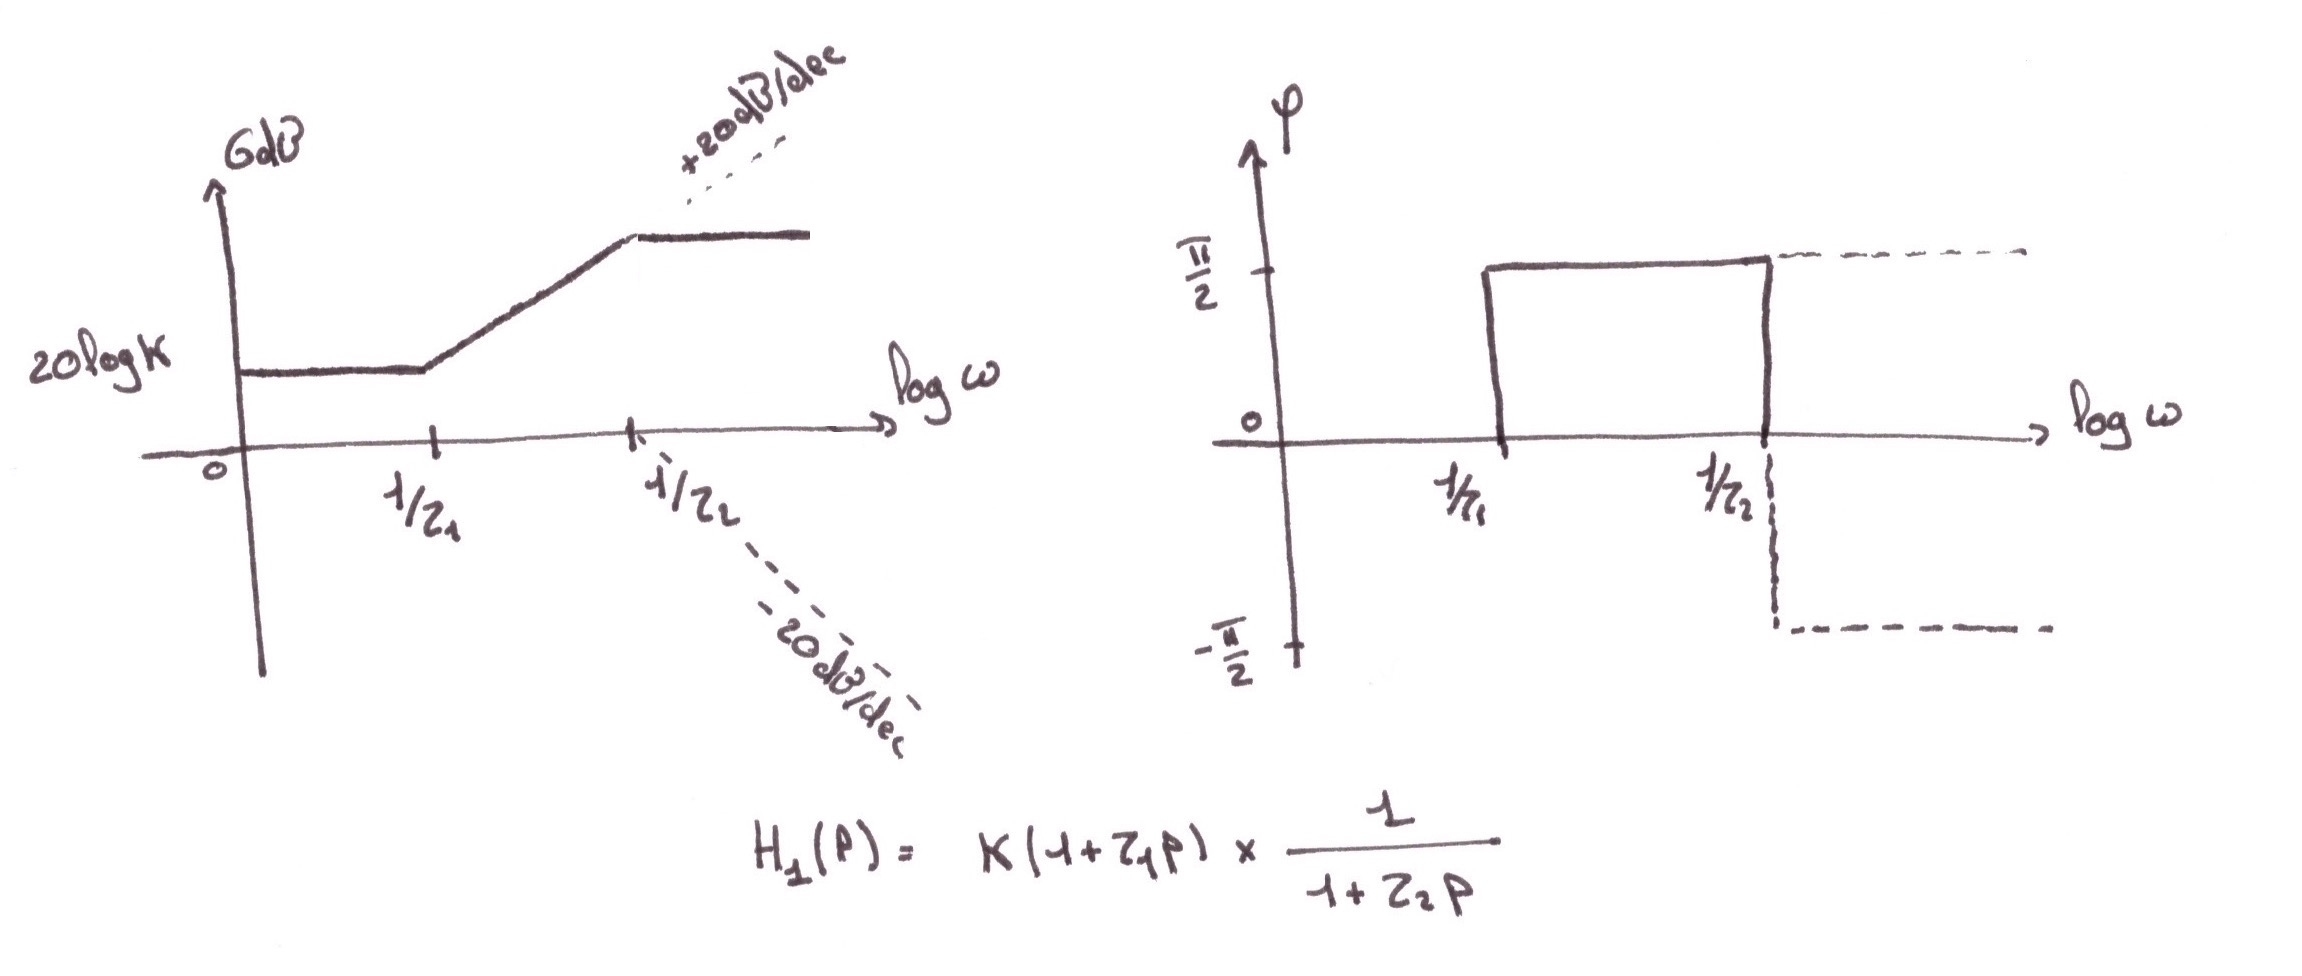
\includegraphics[width=0.5\paperwidth]{png/H1.jpeg}
\end{center}
Diagramme de Bode de $H_2(p)$ :
\begin{center}
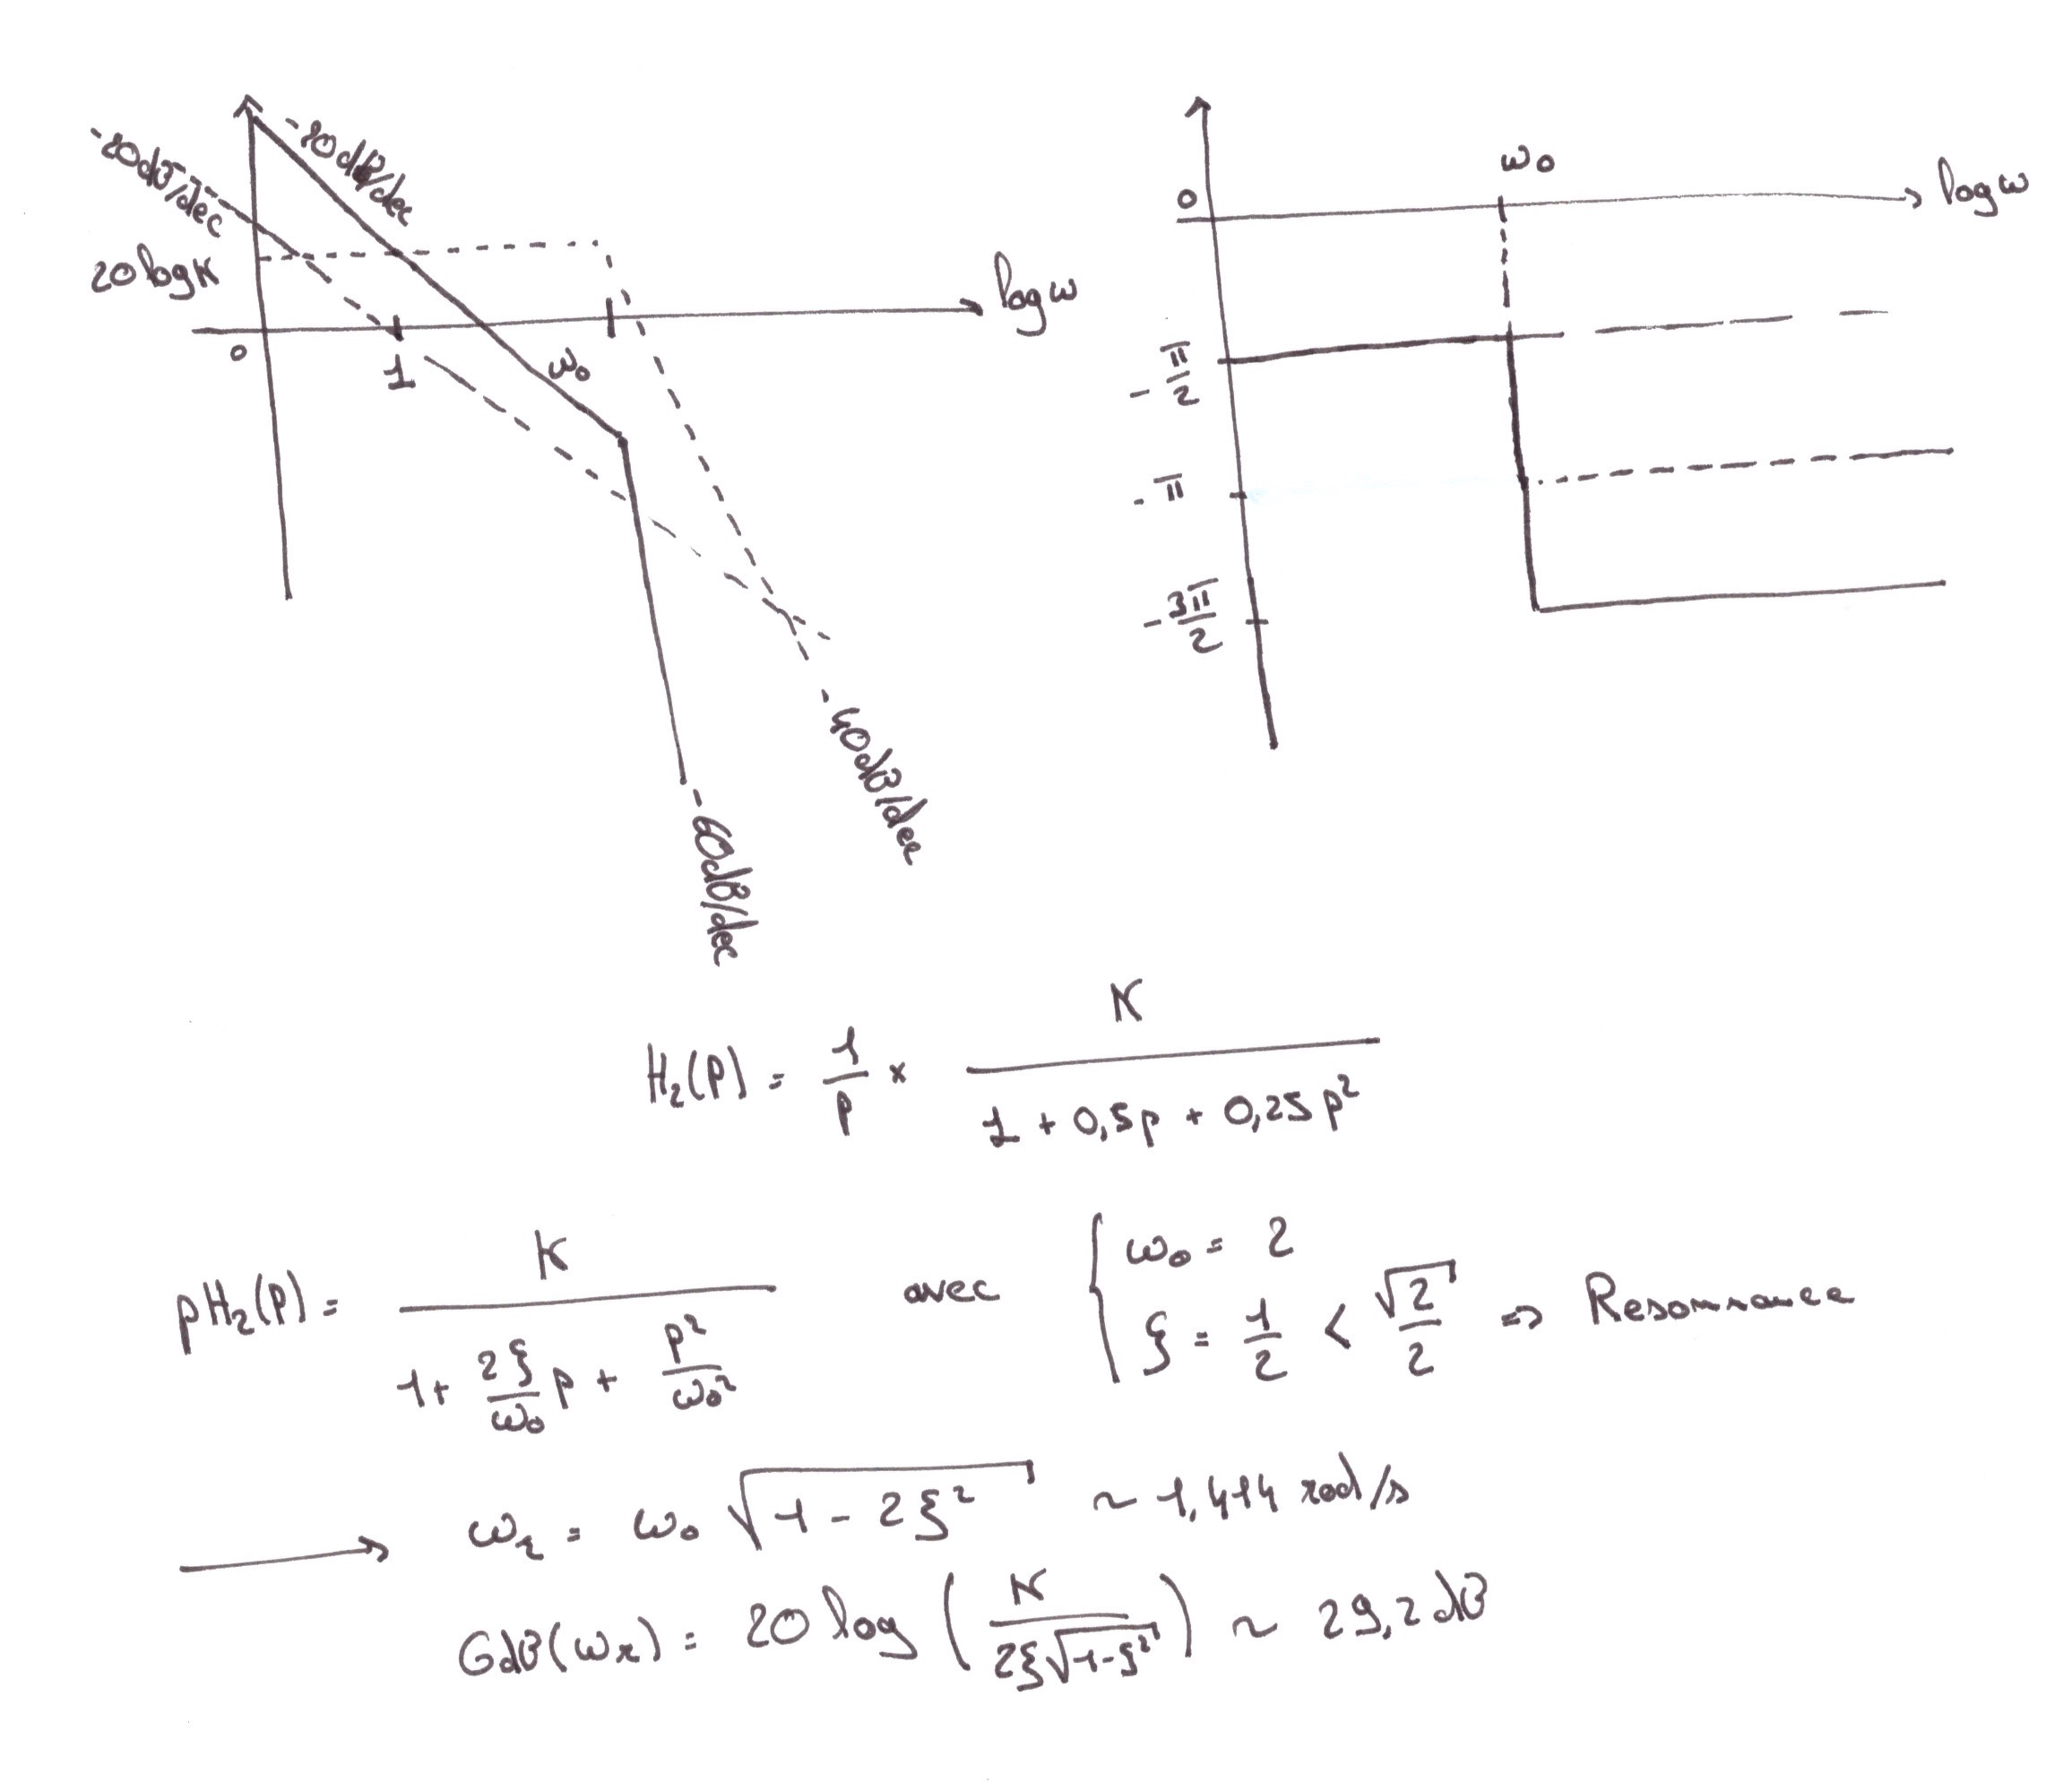
\includegraphics[width=0.5\paperwidth]{png/H2.jpeg}
\end{center}
\item \[ \phi=arg(H_1(j\omega))=arctan(\tau_1 \omega)-arctan(\tau_2 \omega) \] \\
RAPPEL : $arctan'(\theta)=\frac{1}{1+\theta^{2}}$\\
\[ \frac{d \phi}{d \omega}= \frac{\tau_1}{1+(\tau_1 \omega)^{2}}-\frac{\tau_2}{1+(\tau_2 \omega)^{2}}=0 \]
\[ \omega=\sqrt{\frac{1}{\tau_1 \tau_2}}=3,333rad/s \]
d'où $\phi=53^{\circ} $
\end{enumerate}
}
\newpage

%--------------------------------------------

\exercice{Réponse fréquentielle}
On exciste un système linéaire du second ordre par un signal sinusoïdal $e(t)=e_0.\sin(\omega t)$ de fréquence $f=\frac{\omega}{2.\pi}$ variable de $0$ à $500Hz$. Pour $e_0=50mV$, on obtient la sortie $s(t)=s_0.sin(\omega t +\Phi)$ dont l'amplitude $s_0$ est donnée en fonction de la fréquence sur la courbe ci-dessous.

\begin{center}
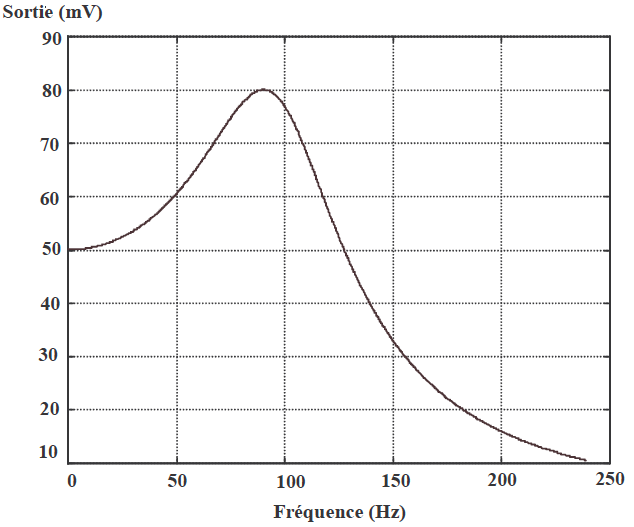
\includegraphics[scale=0.5]{png/graphe2nd.png}
\end{center}

\subsubsection{Travail demandé}
\begin{enumerate}
\item Écrire la fonction de transfert du système et exprimer son module et son argument.
\item Donner les expressions des variables suivantes et utiliser la figure pour calculer leur valeur :
\begin{itemize}
\item le gain statique.
\item la pulsation de résonnance $\omega_R$.
\item le facteur d'amortissement $\xi$.
\item la pulsation propre $f_0$ du système non amortie (pulsation naturelle).
\item la fréquence $f_{C-6dB}$ de coupure à $6dB$.
\end{itemize}
\end{enumerate}

\correction{
\begin{enumerate}
\item \[ H(j\omega)=\frac{K}{1+j2\xi\frac{\omega}{\omega_0}-(\frac{\omega}{\omega_0})^2} \]
Module : \(|H(j\omega)|=\frac{|K|}{\sqrt{(1-(\frac{\omega}{\omega_0})^2)^2+(2\xi \frac{\omega}{\omega_0})^2}} \)\\
Argument : \( arg(H(j\omega))=-\arctan(\frac{2\xi \frac{\omega}{\omega_0}}{1-(\frac{\omega}{\omega_0})^2}) \)\\
\textit{Remarque : $s(t)=|H(j\omega)|e_0 \sin(\omega.t+arg(H(j\omega))$}
\item Expressions :
\begin{itemize}
\item le gain statique : $|H(j\omega=0)|=\frac{|S(j\omega=0)|}{|E(j\omega=0)|}=|K|$ avec  $|S(j\omega=0)|$ l'amplitude de $s(t)$ à la pulsaton nulle et $|E(j\omega=0)|=e_0$ l'amplitude de $e(t)$ à la pulsation nulle. D'où :
\[|K|=\frac{|S(j\omega=0)|}{e_0}=1\]
\item le facteur d'amortissement $\xi<\frac{\sqrt{2}}{2}$ (car résonance).
\item le facteur de surtension $|S(j\omega_r)|=\frac{|K.e_0|}{2\xi \sqrt{1-\xi^2}}$. D'où :
\[ 4\xi^4-4\xi^2+(\frac{|K.e_0|}{|S(j\omega_r)|})^2=0\]
En posant $X=\xi^2$ et en sachant que $0<\xi<\frac{\sqrt{2}}{2}$ : $\xi=0,33$.
\item la pulsation de résonnance : $\omega_r=\omega_0\sqrt{1-2\xi^2}$
\item la pulsation propre $f_0=\frac{\omega_0}{2 \pi}$\\
On en déduit : $f_0=\frac{\omega_0}{2\pi}=\frac{f_r}{\sqrt{1-2\xi^2}}=101,9Hz$.
\item $|S(j\omega_{C-6dB})|=|H(j\omega_{C-6dB})|e_0=10^{\log(|K|)-\frac{6}{20}}e_0=25mV$\\
On en déduit à partir du graphique $f_{C-6dB}=170Hz$.
\end{itemize}
\end{enumerate}
}
\newpage

%----------------------------------------------------------------------------------------
%	PROBLEMES
%----------------------------------------------------------------------------------------
\section{Problèmes}

%--------------------------------------------

\probleme{Mod\'elisation d'une servo-valve}

\subsubsection{I. Pr\'esentation}
On s'int\'eresse ici \`a la loi de comportement d'un v\'erin hydraulique d\'epla\c{c}ant un chariot.
Le syst\`eme se compose de :

\begin{itemize}
\item Un moteur hydraulique lin\'eaire (v\'erin) qui transforme l'\'energie hydraulique en \'energie m\'ecanique. Il est
form\'e de deux chambres 1 et 2, s\'epar\'ees par un piston, de section S, perc\'e d'un trou de fuite de section
tr\`es faible par rapport \`a $S$.
\item Le piston est solidaire d'un chariot, de masse M, dont le d\'eplacement est rep\'er\'e par $x(t)$. Le frottement entre
le chariot et le b\^ati est visqueux (coefficient $\mu$).
\item La circulation du fluide, suppos\'e incompressible, est assur\'ee par une servo-valve dont le d\'ebit volumique
q est proportionnel au courant de r\'eglage $i(t)$ 
\end{itemize}
On note $P_i$ la pression dans la chambre $i$ \`a l'instant $t$. Le d\'ebit de fuite $q_f$ entre les chambres 1 et 2 est
suppos\'e ob\'eir \`a la loi des \'ecoulements laminaires: $q_f(t) = R (p_1(t) - p_2(t))$. On appelle $F(t)$ la force exerc\'ee par l'huile sur
le piston.\\
\hspace*{0mm}
\begin{center}
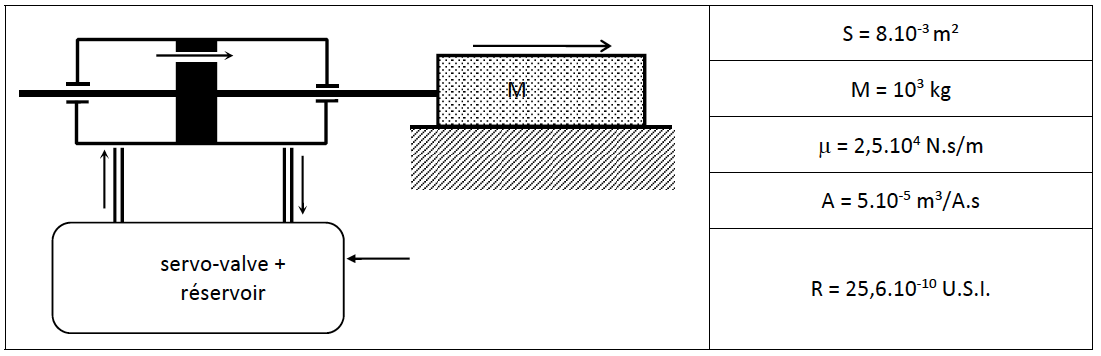
\includegraphics[scale=0.4]{png/img1_prob1.png}
\end{center}
\hspace*{0mm}
Les \'equations d\'ecrivant le comportement des diff\'erents \'el\'ements sont :
\begin{itemize}
\item Comportement de la servo-valve : $ q(t)=A.i(t)$
\item Relation reliant le d\'eplacement du piston aux diff\'erents d\'ebits : $q(t)=q_f(t)+S.\frac{dx(t)}{dt}$
\item Relation liant l'effort de l'huile sur le piston en fonction du d\'ebit de fuite : $F(t)=\frac{S}{R}.q_f(t)$
\item Principe fondamental de la dynamique appliqu\'e au chariot : $M.\frac{d^2x(t)}{dt^2} = F(t)-\mu.\frac{dx(t)}{dt}$
\end{itemize}
\newpage

\subsubsection{II. Travail demand\'e}
\begin{enumerate}
\item D\'efinir l'entr\'ee et la sortie de ce syst\`eme
\item Ecrire les \'equations de comportement dans le domaine de Laplace (on se placera dans les
conditions de Heaviside)
\item Pr\'eciser sur le sch\'ema bloc ci-dessous le nom des grandeurs physiques ainsi que les
fonctions de transfert\\
\hspace*{0mm}
\begin{center} 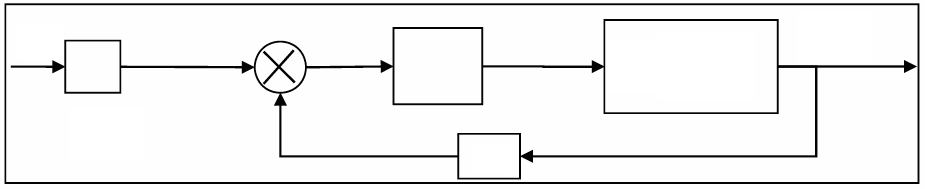
\includegraphics[scale=0.45]{png/img2_prob1.png}\end{center}
\hspace*{0mm}
\item D\'eterminez la fonction de transfert de ce syst\`eme H(p). Pr\'eciser l'ordre de celle-ci.
\item Donner les grandeurs caract\'eristiques de celle-ci en pr\'ecisant les unit\'es.
\item On soumet le syst\`eme \`a un \'echelon d'intensit\'e $I_0$. Pr\'ecisez la fonction de Laplace
correspondante.
\item Donner la relation entre la position et la vitesse puis calculer la vitesse du chariot en r\'egime
permanent.
\item Tracer l'allure de la vitesse.
\item D\'eterminer la r\'eponse $x(t)$ en fonction de $K$, $I_0$ et $\tau$. (on pourra judicieusement s'appuyer
sur l'expression de $v(t)$)
\item On soumet maintenant le syst\`eme \`a une entr\'ee sinuso\"{i}dale d'intensit\'e $I_0$ et de pulsation $\omega_0=\frac{1}{\tau}$. Pr\'ecisez la fonction de Laplace correspondante.
\item D\'eterminer l'expression de $x(t)$ en r\'egime permanent en fonction de $K$, $I_0$ et $\tau$.
\end{enumerate}

\correction{ % Answer
\begin{enumerate}
\item Entrée : courant de réglage de la servo-valve, $i(t)$\\
Sortie : déplacement de la masse $M$, $x(t)$
\item $Q(p)=AI(p)$\\$Q(p)=Q_f(p)+SpX(p)$\\$F(p)=\frac{S}{R}Q_f(p)$\\$Mp^2X(p)=F(p)-\mu p X(p)$
\item Schéma bloc :
\begin{center}
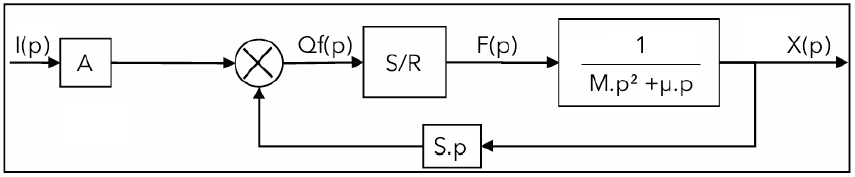
\includegraphics[scale=0.4]{png/img2_prob1-cor.png}
\end{center}
\item Schéma bloc :
\begin{center}
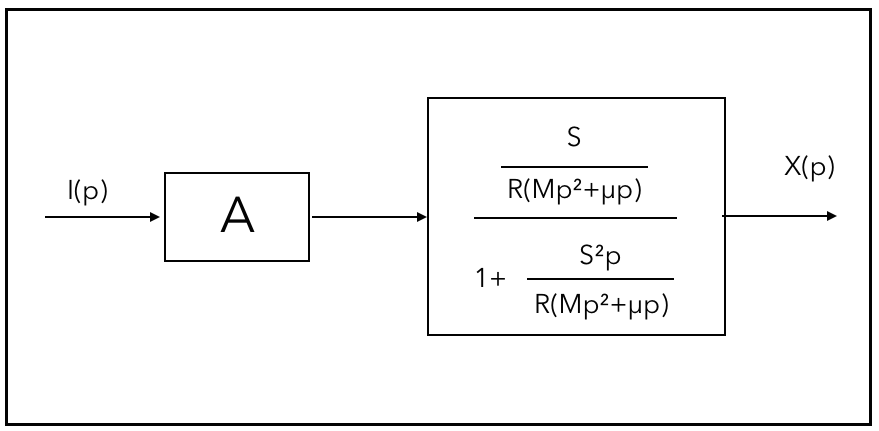
\includegraphics[scale=0.25]{png/img2_prob1-cor2.png}
\end{center}
\[ H(p)=\frac{X(p)}{I(p)}=\frac{\frac{AS}{S^2+R\mu}}{p(1+\frac{RM}{S^2+R\mu}p)} \]
Il s'agit d'une fonction de transfert d'un système du deuxième ordre (première ordre multiplié par un intégrateur pur)
\item On pose \( H(p)=\frac{1}{p}\frac{K}{1+\tau p} \) avec \( K=\frac{AS}{S^2+R\mu} \) (en $m.A^{-1}.s^{-1}$) et \( \tau=\frac{RM}{S^2+R\mu} \) (en $s^{-1}$)\\
\textit{Remarque : l'unité $s^{-1}$ de $K$ vient de l'intégrateur pur}
\item \( I(p)=\frac{I_0}{p} \)
\item Comme \( v(t)=\frac{dx(t)}{dt} \), \( V(p)=pX(p) \)
\[ \lim_{p \rightarrow +\infty} v(t)=\lim_{p \rightarrow 0} pV(p) = \lim_{p \rightarrow 0} p^2X(p)=\lim_{p \rightarrow 0} pH(p)I_0=\lim_{p \rightarrow 0} \frac{KI_O}{1+\tau p}=KI_0 \]
\item Allure de la vitesse $V(t)$ :
\begin{center}
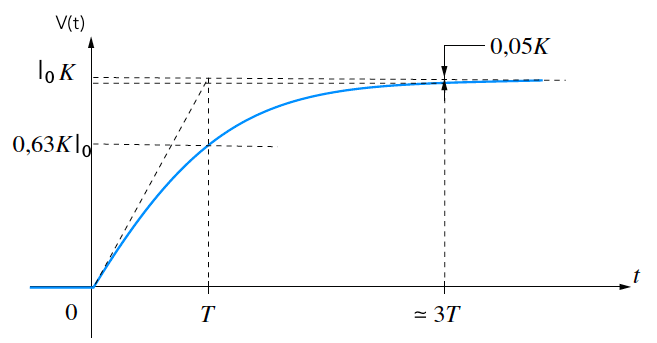
\includegraphics[scale=0.5]{png/courbe-prob1-cor.png}
\end{center}
\item \( v(t)=KI_0(1-e{-\frac{t}{\tau}}) \) car premier ordre\\
\( x(t)=\int_0^t v(t)dt=\int_0^t KI_0(1-e^{-\frac{t}{\tau}})dt=KI_0[t+\tau e^{-\frac{t}{\tau}}-\tau] \)
\item \textit{RAPPEL : $\sin(\omega t)\mathcal{U}(t) \rightarrow \frac{\omega}{p^2+\omega^2}$ et $\cos(\omega t)\mathcal{U}(t) \rightarrow \frac{p}{p^2+\omega^2}$}\\
\( i(t)=I_0\sin(\omega_0 t) \rightarrow I(p)=\frac{I_0\omega_0}{p^2+\omega_0^2}=\frac{\frac{I_0}{\tau}}{p^2+\frac{1}{\tau^2}} \) où $\omega_0=\frac{1}{\tau}$
\item \[ X(p)=\frac{1}{p}\frac{K}{1+\tau p}\frac{I_0\frac{1}{\tau}}{p^2+\frac{1}{\tau^2}}=\frac{KI_0 \tau}{p}-\frac{\frac{KI_0 \tau}{2}}{\frac{1}{\tau}+p}-\frac{\frac{KI_0 \tau}{2}(p+\frac{1}{\tau})}{p^2+\frac{1}{\tau^2}} \]
\[ x(t)=\frac{KI_0 \tau}{2}(2-\cos(\frac{t}{\tau})-\sin(\frac{t}{\tau})-e^{-\frac{t}{\tau}}) \]
En régime permanent : \( x(t)=\frac{KI_0 \tau}{2}(2-\cos(\frac{t}{\tau})-\sin(\frac{t}{\tau})) \)
\end{enumerate}
}
\newpage

%--------------------------------------------

\probleme{Cam\'era de poursuite (SPEEDCAM)}

\subsubsection{I. Pr\'esentation}
L'\'etude porte sur la cam\'era de poursuite SPEDDCAM utilis\'ee dans de nombreux championnats pour filmer les performances des sportifs. La cam\'era est fix\'ee sur un chariot se d\'epla\c{c}ant sur un rail.
\\ \hspace*{0mm}
\begin{center}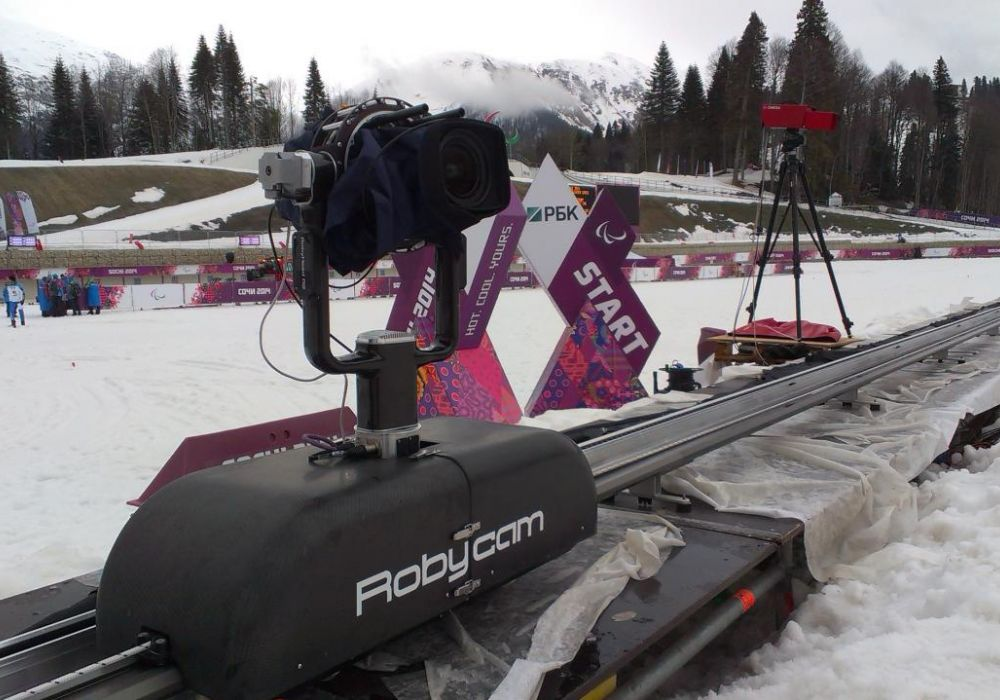
\includegraphics[scale=0.22]{png/img1_prob2.jpg} 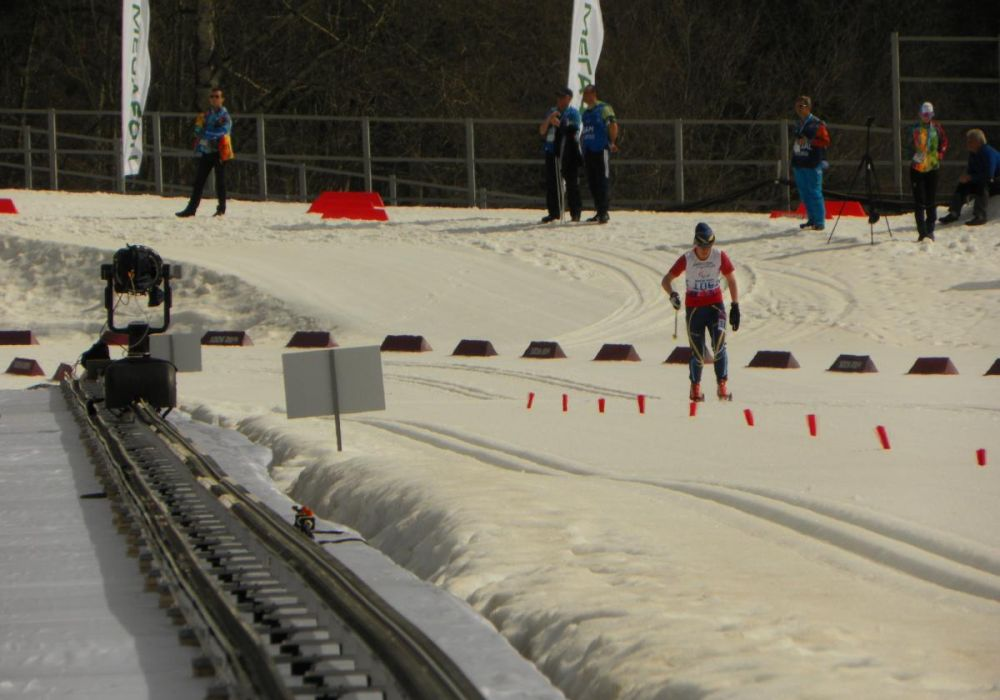
\includegraphics[scale=0.22]{png/img2_prob2.jpg}\end{center}
\hspace*{0mm}
\\Un capteur optique permet de mesurer la position de la cam\'era par rapport au comp\'etiteur. Un calculateur d\'etermine la consigne n\'ecessaire pour suivre le comp\'etiteur, transmise sous forme de tension de commande \`a l'asservissement du chariot. Le chariot est asservi en vitesse comme le montre le sch\'ema fonctionnel suivant :
\\ \hspace*{0mm}
\begin{center}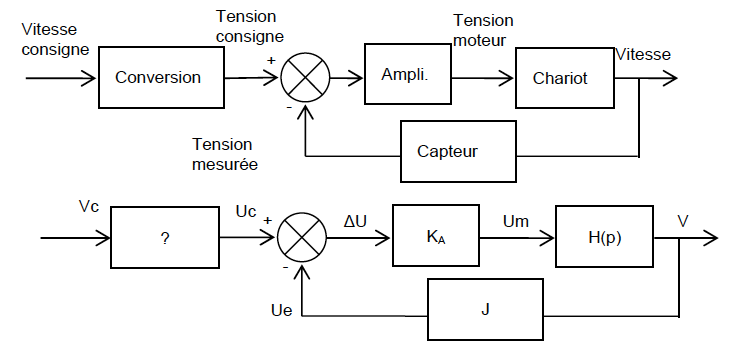
\includegraphics[scale=0.6]{png/bloc1_prob2.png}\end{center}
\hspace*{0mm}
\\ Le chariot est actionn\'e par un moteur \'electrique pilot\'e par sa tension d'entr\'ee $u_m(t)$. Cette tension est obtenue \`a l'aide d'un amplificateur fournissant une tension $u_m(t)$ proportionnelle \`a la tension de commande $\Delta U$ (gain $K_A = 500$). Un capteur de vitesse mesure la vitesse $v(t)$ et renvoit une information de tension $u_e(t)$
proportionnelle \`a la vitesse $v$ (gain $J = 0,3 V.s/m$).


\begin{enumerate}
\item D\'eterminer la fonction \`a mettre dans le convertisseur ("$?$") pour que $V$ soit asservie sur
$Vc$ (donc pour que $V$ soit compar\'ee \`a $Vc$).
\end{enumerate}

\subsubsection{II. Mod\'elisation du comportement du chariot}
Le chariot \'etant relativement complexe, il est impossible de donner a priori un mod\`ele de comportement $H(p)$ comme pour le capteur de vitesse ou l'amplificateur. Afin de mod\'eliser son comportement, on choisit de faire une mesure et de proposer un mod\`ele simple repr\'esentatif. La courbe (cf. graphe suivant) montre la r\'eponse obtenue par le capteur de vitesse lorsqu'un \'echelon de tension $u_m(t) = u_0.u(t)$ (avec $u_0 = 70 V$) est appliqu\'e en entr\'ee. ($u(t)$ : fonction de heaviside).
\\ On choisit un mod\`ele simple du premier ordre pour identifier le comportement du chariot, soit : \(H(p)=\frac{K_c}{1+\tau .p}\) o\`u $K_c$ et $\tau$ sont \`a d\'eterminer \`a l'aide de la courbe.

\begin{enumerate}
\item Exprimer $U_e(p)$ en fonction de $U_m(p)$.
\item D\'eterminer $K_c$ \`a l'aide de la courbe. Quelle est son unit\'e ?
\item D\'eterminer $\tau$ \`a l'aide la courbe par trois m\'ethodes. A partir des trois valeurs obtenues,
proposer une valeur de $\tau$ pertinente.\\
\hspace*{0mm}
\begin{center} \includegraphics[scale=0.45]{png/courbe_prob2.png}\end{center}
\hspace*{0mm}
\end{enumerate}
\newpage

\subsubsection{III. Etude des performances du syst\`eme en boucle ferm\'ee}
On cherche maintenant \`a caract\'eriser les performances du syst\`eme asservi, c'est \`a dire la stabilit\'e, la rapidit\'e et la pr\'ecision.

\begin{enumerate}
\item Calculer la fonction de transfert \(H_T(p) = \frac{V(p)}{V_c(p)}\) du chariot asservi. D\'eterminer les caract\'eristiques de cette fonction de transfert.

\item En calculant la valeur \`a convergence de $v(t)$ suite \`a une entr\'ee en \'echelon $v_c(t)=V_{c0}.u(t)$. D\'eterminer si le syst\`eme est pr\'ecis. Comment augmenter cette pr\'ecision ?

\item D\'eterminer la rapidit\'e du syst\`eme. Comment augmenter la rapidit\'e ? Quelle sera la cons\'equence sur la pr\'ecision ?
\end{enumerate}

\subsubsection{IV. Am\'elioration de la pr\'ecision}
Une m\'ethode classique pour augmenter la pr\'ecision est d'ajouter un int\'egrateur $\frac{1}{p}$ dans la cha\^ine directe (voir figure ci dessous). Cet ajout est facile en amont de l'amplificateur. On d\'esigne par " correcteur " cet \'el\'ement rajout\'e, destin\'e \`a am\'eliorer le comportement de l'asservissement.
\\ \hspace*{0mm}
\begin{center} \includegraphics[scale=0.5]{png/bloc2_prob2.png}\end{center}
\hspace*{0mm}

\begin{enumerate}
\item Calculer la fonction de transfert \(H_{cor}(p)=\frac{V(p)}{V_c(p)}\) du chariot asservi. Pr\'eciser l'ordre de la fonction obtenue.
\item D\'eterminer si le syst\`eme est pr\'ecis.
\end{enumerate}

\correction{ % Answer
\textbf{Partie I}
\begin{enumerate}
\item La fonction du convertisseur est un gain $J$ qui convertit une vitesse en tension.
\end{enumerate}

\textbf{Partie II}
\begin{enumerate}
\item \( U_e(p)=H(p).J.U_m(p) \)
\item Lecture graphique de la coube $U_e(t)$ :
\begin{center}
\includegraphics[scale=0.5]{png/courbe-prob2-cor.png}
\end{center}
\item \( \tau=0,5s \)
\end{enumerate}

\textbf{Partie III}
\begin{enumerate}
\item \( H_T(p)=\frac{V(p)}{V_c(p)}=\frac{JK_AH(p)}{1+JK_AH(p)}=\frac{\frac{K_cK_AJ}{1+JK_AK_c}}{1+\frac{\tau}{1+JK_AK_c}p} \)\\
\(H_T(p)=\frac{K_T}{1+\tau_Tp} \) avec \( K_T=\frac{K_cK_AJ}{1+JK_AK_c} \) et \( \tau_T=\frac{\tau}{1+JK_AK_c} \)
\item \( v_c(t)=v_{c0}\mathcal{U(t)} \rightarrow V_c(p)=\frac{V_{c0}}{p} \)\\
\( \lim_{t \to +\infty}v(t)=\lim_{p \to 0}pV(p)=\lim_{p \to 0}\frac{K_T}{1+\tau_T p}V_{c0}=K_TV_{c0} \)\\
Le système est précis seulement si $v(t) \rightarrow_{t \to +\infty} V_{c0}$ donc $K_T$ doit tendre vers $1$. Comme $K_T=\frac{K_cK_AJ}{1+JK_AK_c}$ il faut pouvoir augmenter $K_A$, en pratique $K_A \rightarrow +\infty$ est impossible.
\item Pour un premier ordre, $t_{5\%} \simeq 3\tau_T = \frac{3\tau}{1+JK_AK_c}$\\
Pour augmenter la rapidité, il faut augmenter $K_A$.
\end{enumerate}

\textbf{Partie IV}
\begin{enumerate}
\item \( H_{cor}(p)=\frac{V(p)}{V_c(p)}=J\frac{H(p)\frac{K_A}{p}}{1+H(p)J\frac{K_A}{p}}=\frac{1}{1+\frac{1}{JK_AK_c}p+\frac{\tau}{JK_AK_c}p^2} \)\\
Il s'agit d'une fonction de transfert du deuxième ordre.
\item \( \lim_{t \to +\infty}[v(t)-v_c(t)]=\lim_{p \to 0}p[V(p)-V_c(p)]=\lim_{p \to 0}[H_{cor}(p)-1]V_{c0}=0 \)\\
L'erreur statique étant nulle, le système est précis.
\end{enumerate}
}
\newpage

%--------------------------------------------

\probleme{Asservissement de l'arbre \`a came d'un tracteur Fendt}

\subsubsection{I. Performances exig\'ees}
\begin{itemize}
\item Pr\'ecision : pas d'\'ecart de position
\item Rapidit\'e : temps de r\'eponse \`a $5\%$ global du syst\`eme \`a une consigne d'entr\'ee de type \'echelon inf\'erieur \`a $1s$.
\end{itemize}

\subsubsection{II. Mod\'elisation du servomoteur \`a courant continu}
On s'int\'eresse \`a l'asservissement en position de l'arbre de commande dont le sch\'ema fonctionnel est donn\'e ci-dessous.\\

\begin{center}
\includegraphics[scale=0.4]{png/image2_prob4.png}
\end{center}

Le moteur \'electrique est un moteur \`a courant continu dont les \'equations caract\'eristiques sont les suivantes :\\
\[u(t)=R.i(t)+k_e . \frac{d \theta(t)}{dt} \ \ \textrm{et} \ \ J_e . \frac{d^2 \theta(t)}{dt^2} = k_a . i(t)\]
avec :
\begin{itemize}
\item $u(t)$ : tension appliqu\'ee aux bornes du moteur
\item $i(t)$ : courant d'induit
\item $R = 2 \Omega$ : r\'esistance de l'induit
\item $J_e = 6,25.10^{-4} kg.m^2$ : inertie de l'arbre de commande
\item $k_e = 0,5 V / (rad / s)$ : constante de force contre \'electromotrice
\item $k_a = 0,05 Nm/A$ : constante de couple
\end{itemize}
Le gain du capteur de vitesse $K_r = 2V.rad^{-1}$\\
On consid\`ere nulles les conditions initiales.

\begin{enumerate}
\item D\'eterminer la fonction de transfert $M(p) = \frac{\Theta(p)}{U(p)}$ du moteur \'electrique et montrer qu'elle peut se mettre sous la forme canonique : $M(p) = \frac{K_m}{p.(1+\tau_m . p)}$.
\item Donner les expressions litt\'erales de $K_m$ et $\tau_m$. Calculer $K_m$ et $\tau_m$.
\item D\'eterminer la fonction de transfert $F(p)=\frac{\Theta(p)}{U_e(p)}$, donner l'ordre de cette fonction de transfert.
\item Mettre $F(p)$ sous forme canonique en pr\'ecisant l'expression de ces caract\'eristiques.
\item D\'eterminer la valeur du gain $K_c$ de telle sorte que la r\'eponse \`a une entr\'ee de type \'echelon soit la plus rapide possible sans toutefois produire de d\'epassement.
\item Montrer qu'avec la valeur de $K_c$ choisie pr\'ec\'edemment, la fonction de transfert en boucle ferm\'ee peut se mettre sous la forme : $ F(p) = \frac{K_{BF}}{(1+T.p)^2} $
\item Calculer $K_{BF}$ et $T$.\\
La courbe ci-dessous repr\'esente la r\'eponse du moteur \`a un \'echelon d'amplitude $2V$.

\begin{center}
\includegraphics[scale=0.25]{png/image3_prob4.png}
\end{center}

\item En d\'eduire le temps de r\'eponse \`a $5\%$. Conclure vis-\`a-vis des exigences du cahier des charges.\\
On souhaite diviser par dix le temps de r\'eponse du syst\`eme afin de satisfaire les exigences du cahier des charges. On introduit une boucle de retour suppl\'ementaire dite boucle de vitesse ou retour tachym\'etrique comme l'illustre la figure ci-dessous.

\begin{center}
\includegraphics[scale=0.4]{png/image4_prob4.png}
\end{center}

\item D\'eterminer la nouvelle fonction de transfert $M'(p)$ du moteur et montrer qu'elle peut s'\'ecrire :\\
\[M'(p) = \frac{\Theta(p)}{U(p)}=\frac{K'_m}{p.(1+\tau '_m . p)}\]
\item Donner les expressions litt\'erales de $K'_m$ et $\tau'_m$ en fonction notamment de $K_m$ et $\tau_m$.
\item D\'eterminer la valeur $k$ du gain du retour tachym\'etrique de telle sorte que $\tau'_m = \frac{\tau_m}{10}$.
\item D\'eterminer les nouvelles valeurs de $K'_m$, $K_C$, $K_{BF}$ et $T$.
\item En d\'eduire l'\'ecart de position du syst\`eme \'equivalent.
\end{enumerate}

\subsubsection{III. Annexe}
\begin{center}
\includegraphics[scale=0.4]{png/image5_prob4.png}\\
\includegraphics[scale=0.4]{png/image6_prob4.png}
\end{center}

\correction{ % Answer
\begin{enumerate}
\item \[ M(p)=\frac{\theta(p)}{U(p)}=\frac{\frac{1}{K_e}}{p(1+\frac{RJ_e}{K_eK_a}p)} \]
\item \( K_m=\frac{1}{K_e}=2 rad.s^{-1}.V^{-1} \) et \( \tau_m=\frac{RJ_e}{K_eK_a}=0,05s \)
\item \[ F(p)=\frac{\theta(p)}{U_e(p)}=\frac{\frac{1}{K_r}}{1+\frac{1}{K_rK_cK_m}p+\frac{\tau_m}{K_rK_cK_m}p^2} \]
Il s'agit d'une fonction du second ordre.
\item On pose $F(p)=\frac{K}{1+\frac{2\xi}{\omega_0}p+\frac{1}{\omega_0^2}p^2}$. On en déduit :
\begin{description}
\item \( K=\frac{1}{K_r} \)
\item \( \omega_0=\sqrt{\frac{K_rK_cK_m}{\tau_m}} \)
\item \( \xi=\frac{1}{2\sqrt{K_rK_cK_m\tau_m}} \)
\end{description}
\item On veut $\xi=1$ d'où \( K_c=\frac{1}{4K_rK_m\tau_m}=1,25 \)
\item \[ F(p)=\frac{\theta(p)}{U_e(p)}=\frac{0,5}{1+0,2p+0,01p^2}=\frac{0,5}{(1+0,1)^2} \]
\item \[K_{BF}=0,5 rad.V^{-1} \]
\[ T=0,1 s \]
\item Comme $T_{r5\%}>1s$, le cahier des charges n'est pas respecté.
\item \[ M'(p)=\frac{\theta(p)}{U(p)}=\frac{\frac{K_m}{1+kK_m}}{p(1+\frac{\tau_m}{1+kK_m}p)} \]
\item \[ K'm=\frac{K_m}{1+kK_m} \]
\[\tau'_m=\frac{\tau_m}{1+kK_m} \]
\item Comme $\tau'_m=\frac{\tau_m}{10}$, on obtient $1+kK_m=10$. D'où \( k=\frac{9}{K_m}=4,5V.(rad.s^{-1})^{-1} \)
\item \[ K'_m=0,2 rad.s^{-1}.V^{-1} \]
\[ K_c=1,25 \]
\[ K_{BF}=0,5 rad.V^{-1} \]
\[ T=0,1s \]
\item L'écart de position est nul $ \lim_{t\rightarrow \infty}\epsilon(t)=0 $
\end{enumerate}
}
\newpage

%--------------------------------------------

\probleme{Machine de fa\c{c}onnage \`a plat}

\subsubsection{I. Pr\'esentation}
Le fa\c{c}onnage \`a plat consiste \`a d\'ecouper, rainer (ou rainurer) et gaufrer des feuilles de papier, carton
ou carton ondul\'e pour r\'ealiser des menus, des \'etiquettes, des d\'epliants apr\`es pliage ou encore des bo\^ites
apr\`es pliage et collage... Les principales \'etapes du processus de fa\c{c}onnage sont repr\'esent\'ees sur la figure ci-dessous.
On d\'epose une palette de feuilles empil\'ees sur le margeur. Les feuilles sont prises depuis le dessus
de la pile et envoy\'ees sur la table de marge pour \^etre mises en nappe et positionn\'ees par rapport \`a leurs
bords, avant d'\^etre introduites dans la presse par un syst\`eme de transport de barres \`a pinces entra\^in\'ees par
un convoyeur \`a cha\^ines pour y subir l'op\'eration de d\'ecoupage/rainage/gaufrage. Les d\'echets constitu\'es des
zones non utilis\'ees de la feuille comme les bandes arri\`eres et les c\^ot\'es sont enlev\'es et les poses (feuilles
d\'ecoup\'ees) sont empil\'ees en un seul tas sur une palette.

\begin{center}
\includegraphics[scale=0.35]{png/image1_prob3.png}
\end{center}

\subsubsection{II. Mod\'elisation du servomoteur \`a courant continu}
L'objectif de cette partie est de choisir un mod\`ele pertinent du moteur \`a courant continu et de le
valider \`a partir de relev\'es exp\'erimentaux, mod\`ele qui sera utilis\'e pour le r\'eglage des param\`etres de
l'asservissement.\\
Les caract\'eristiques du moteur utilis\'e pour entra\^iner le dispositif de r\'eglage du sommier sont les
suivantes :
\begin{itemize}
\item moment d'inertie ramen\'e \`a l'arbre moteur : $J_{eq} = 0,306 kg.m^2$
\item r\'esistance de l'induit : $R=0,5 \Omega$
\item constante de couple et de vitesse : $K=K_c = K_e = 0,244 U.S.I$
\item inductance de l'induit : $L=1 mH$
\end{itemize}
Par ailleurs, on suppose que les frottements sont n\'egligeables. On rappelle enfin les \'equations qui d\'ecrivent le fonctionnement du moteur sont :
\begin{itemize}
\item Equations \'electriques :
\begin{description}
\item \(U_c(t) = R.i(t)+L. \frac{di(t)}{dt} + e(t) \)
\item \(e(t)=K_e.\omega(t) \)
\item \(C_m(t)=K_c.i(t) \)
\end{description}
\item Equation m\'ecanique :
\begin{description}
\item \(J_{eq}. \frac{d \omega(t)}{dt} = C_m(t)-C_r(t) \)
\item avec $C_r(t)$ : couple r\'esistant. 
\end{description}
\end{itemize}
La figure ci-dessous repr\'esente le relev\'e exp\'erimental de la r\'eponse de la cha\^ine fonctionnelle \`a un
\'echelon unitaire de la tension dans le cas o\`u $C_r(t)$ est nul.

\begin{center}
\includegraphics[scale=0.4]{png/image2_prob3.png}
\end{center}

\begin{enumerate}
\item Justifier que l'on peut identifier cette r\'eponse \`a celle d'un syst\`eme du premier ordre.
\item D\'eterminer graphiquement les param\`etres caract\`eristiques du mod\`ele.\\
Nous allons maintenant \'etablir le mod\`ele de connaissance du moteur afin de le confronter au mod\`ele
de comportement que nous venons d'\'etablir.
\item Compl\'eter le sch\'ema fonctionnel du moteur et de sa charge propos\'e dans le document
r\'eponse DR1.\\

\begin{center}
\includegraphics[scale=0.3]{png/image3_prob3.png}
\end{center}

\item Montrer que l'on peut \'ecrire $\Omega(p)$ sous la forme : $\Omega(p)=H_1(p).U_c(p)+H_2(p).C_r(p)$\\
Donner les expressions litt\'erales de $H_1(p)$ et $H_2(p)$.\\
On \'etudie maintenant l'\'evolution du syst\`eme autour d'un point de fonctionnement vis-\`a-vis de la consigne.
Dans ces conditions le couple r\'esistant est suppos\'e constant. En cons\'equence on posera $C_r(p)=0$ pour la suite.
\item Montrer que la fonction de transfert en boucle ouverte (lorsque l'on ouvre la boucle avant
le comparateur) peut se mettre sous la forme :\\
\[T_{MBO}(p)=\frac{E(p)}{U_c(p)}=\frac{1}{\tau .p.(1+ \tau_e . p)}\]\\
Donner les expressions de $\tau_m$ et $\tau_e$ en fonctions des param\`etres du syst\`eme. Puis calculer leur valeur num\'erique.
\item Exprimer $H_1(p)$ en fonction de $\tau_m$, $\tau_e$ et $K_e$. Ce r\'esultat est-il compatible avec le trac\'e obtenu exp\'erimentalement ?\\
Dans le suite du probl\`eme on admettra que $H_1(p)$ s'\'ecrit : $H_1(p)= \frac{G_0}{1+\tau_m . p}$
\end{enumerate}

\subsubsection{III. \'Etude de la boucle de position}
L'objectif de cette partie est de r\'egler le correcteur de l'asservissement de position des pieds de r\'eglage pour que le d\'eplacement s'effectue dans le temps impos\'e par le cahier des charges, c'est-\`a-dire moins de $0,2s$.\\
Le moteur \`a courant continue entraine la cale de r\'eglage de parall\'elisme du sommier par l'interm\'ediaire d'un r\'educteur de rapport de r\'eduction $R_e$, et d'un syst\`eme vis \'ecrou dont le pas r\'eduit est not\'e $h=\frac{P_v}{2*\pi}$ en $mm$.\\
$Z(p)$ correspond au d\'eplacement de la cale suivant l'axe $\overrightarrow{z_0}$, et $E_s(p)$ au d\'eplacement vertical du sommier suivant $\overrightarrow{y_0}$, en $C$. Ces diff\'erents \'el\'ements sont d\'efinis sur la figure ci-dessous :\\

\begin{center}
\includegraphics[scale=0.3]{png/image4_prob3.png}
\end{center}

On appelle $E_c(p)$ la tension de consigne de correction duparall\'elisme entre le sommier et la presse au point mort bas. La position, not\'ee $e_s$, est mesur\'ee par un capteur de position de gain $T_{cap}$. L'unit\'e utilis\'ee pour $e_s$ est le $mm$.\\
Le moteur \`a courant continu est aliment\'e par un convertisseur qui sera consid\'er\'e comme un gain pur, not\'e $K_h = 20$.

\begin{enumerate}
\item Compl\'eter sur le document r\'eponse DR2 le sch\'ema bloc de l'asservissement de position.\\
Remarque : le bloc $C(p)$ symbolise un correcteur qui ne sera pas \'etudi\'e dans ce probl\`eme.\\

\begin{center}
\includegraphics[scale=0.3]{png/image5_prob3.png}
\end{center}

\item Exprimer la relation qui lie $z$ et $e_s$ en vous appuyant sur le sch\'ema ci-dessus. En d\'eduire l'expression de $K_z$.\\
On donnes pour la suite $K_z = 0,1$.
\item Montrer graphiquement que le sch\'ema bloc du DR2 peut se mettre sous la forme d'un syst\`eme boucl\'e \`a retour unitaire.\\
Dans la suite du probl\`eme on prendra pour fonction de transfert du capteur de position $T_{cap}=1 V.mm^{-1}$.
\item Exprimer $F_{TBO}(p)$, fonction de transfert de la zone entour\'ee d'un pointill\'e sur le DR2. La mettre sous la forme $F_{TBO}(p)=C(p).\frac{G}{D(p)}$. Calculer $G$.\\
Le cahier des charges impose les caract\'eristiques minimales suivantes :
\begin{itemize}
\item valeur du premier d\'epassement en r\'egime indiciel $D_{1\%}\leq 20\%$
\item instant du premier maximum en r\'egime indiciel $T_{max} \leq 0,1s$
\item temps de r\'eponse \`a $5\%$ inf\'erieur \`a $0,2s$
\end{itemize}
Apr\`es un choix de correction pour $C(p)$, on obtient la r\'eponse ci-dessous \`a un \'echelon unitaire de position du syst\`eme corrig\'e.

\begin{center}
\includegraphics[scale=0.3]{png/image6_prob3.png}
\end{center}

\item Conclure quant au respect du cahier des charges.

\end{enumerate}

\correction{ % Answer
\textbf{Partie II}
\begin{enumerate}
\item Tangente à l'origine non nulle.
\item \begin{center}
\includegraphics[scale=0.5]{png/courbe-cor-pb3.png}
\end{center}
Comme $E_0=1$, on en déduit $K=1rad.s^{-1}.V^{-1}$ et $\tau=2,5s$
\item Schema bloc :
\begin{center}
\includegraphics[scale=0.5]{png/SB-pb3.png}
\end{center}
\item \[\Omega(p)=H_1(p)U_c(p)+H_2(p)C_r(p)\]
avec \(H_1(p)=\frac{K_c}{K_cK_e+Jp(R+Lp)} \) et \( H_2(p)=\frac{R+Lp}{K_cK_e+Jp(R+Lp)}\)
\item \[T_{MBO}(p)=\frac{1}{\frac{JR}{K_cK_e}(1+\frac{L}{R}p}=\frac{1}{\tau p(1+\tau_e p)}\]
\underline{Application numérique :} $\tau = 2,57 s$ et $\tau_e=2 ms$
\item \[H_1(p)=\frac{\frac{1}{K_e}}{1+\frac{RJ}{K_cK_e}p+\frac{LJ}{K_cK_e}p^2}=\frac{\frac{1}{K_e}}{1+\tau_m p+\tau_m \tau_e p^2}\]
$H_1(p)$ est une fonction de transfert du deuxième ordre, mais comme $\tau_e$ est négligeable devant $\tau_m$ (Rapport $1000$), nous pouvons nous ramener à une fonction de transfert du première ordre dont la constante de temps est $\tau_m=2,5s$. Cette hypothèse concorde avec la courbe expérimentale étudiée.
\end{enumerate}

\textbf{Partie III}
\begin{enumerate}
\item Schéma bloc :
\begin{center}
\includegraphics[scale=0.5]{png/SB2-cor-pb3.png}
\end{center}
\item \[\tan \alpha = K z\]
\item Schéma bloc :
\begin{center}
\includegraphics[scale=0.5]{png/SB3-cor-pb3.png}
\end{center}
\item \[F_{TBO}(p)=C(p)\frac{K_HH_1(p)R_eP_vKz}{2 \pi p}T_{cap}=C(p)\frac{G}{D(p)}\]
où \( G=\frac{K_HR_eP_vKz}{2 \pi} G_0T_{cap}=0,26mm.V^{-1} \) et \( D(p)=p(1+\tau_m p) \)
\item Vérification du cahier des charges :
\begin{itemize}
\item $D_{1}\%=18\%<20\%$ : OK
\item $T_{max}=0,08<0,1$ : OK
\item $T_{r5\%}<0,2s$ : OK
\end{itemize}
\end{enumerate}
}
\newpage
 % Systèmes linéaires, continus et invariants
\chapter{Cinématique et Modélisation du solide indéformable}
\thispagestyle{plain} % Supprimer le header & le footer sur cette page en laissant la numérotation
\newpage

%----------------------------------------------------------------------------------------
%	Vecteurs positions, vitesse et accélération d'un point d'un solide
%----------------------------------------------------------------------------------------

\section{Vecteurs positions, vitesse et accélération d'un point d'un solide}

%--------------------------------------------

\exercice{Système bielle-manivelle}

Le schéma cinématique de la Figure $13$ modélise un système de bielle-manivelle.\\
Soit $R(O,\vec{x},\vec{y},\vec{z})$ Un repère lié au bâti $0$. La manivelle $1$ est en liaison pivot d'axe $(O,\vec{z})$ avec le bâti $0$. Le coulisseau $2$ est en liaison pivot glissant d'axe $(O,\vec{x})$ avec le bâti $0$. La bielle $3$ est en liaison rotule avec $1$ et $2$ de centre respectif $P$ et $Q$, situés dans le plan $(O,\vec{x},\vec{y},\vec{z})$.\\
On pose $\theta=(\vec{x},\overrightarrow{OP})$ avec :
\begin{description}
\item $\theta=\omega.t$ ($\omega=452,4 rad/s$)
\item $r=OP$ ($r=30 mm$)
\item $l=PQ$ ($l=70 mm$)
\end{description}
Définissons la position du point $Q$ du coulisseau $2$ par rapport au bâti $0$ par la varibale $x(t)=\overline{OQ}$. Comme $\theta=\omega.t$, $x(t)$ peut-être également considérée comme une fonction de $\theta$ : $x(\theta)$.

\begin{center}
    \includegraphics[scale=0.6]{png/bielle.png}
\end{center}

\subsubsection{Travail demandé}
\begin{enumerate}
\item Déterminer graphiquement la courbe représentative de la position du coulisseau par rapport au bâti en fonction de la position angulaire de la manivelle : $x(\theta)$ pour $\theta \in [0,2\pi]$.
\item En déduire par dérivation graphique la courbe représentative de la vitesse du coulisseau par rapport au bâti en fonction de la position angaire de la manivelle : $\theta'_t(\theta)=\frac{dx(\theta)}{dt}$ pour $\theta \in [0,2\pi]$.
\item En déduire par dérivation graphique la courbe représentative de l'accélération du coulisseau par rapport au bâti en fonction de la position angaire de la manivelle : $\theta''_t(\theta)=\frac{dx'_t(\theta)}{dt}$ pour $\theta \in [0,2\pi]$.
\end{enumerate}


\correction{ % Answer
\begin{center}
    \includegraphics[scale=0.8]{png/bielle_correction.png}
\end{center}
}
\newpage
%--------------------------------------------

\exercice{Les KBOTS de l'ENS Cachan}

\begin{center}
\includegraphics[scale =0.1]{png/1_exo3.png}
\end{center}

Le club de robotique de l\rq{}ENS Cachan, [Kro]Bot, ont développé entre le mois de septembre et le mois de décembre des KBOTS.
Un KBOTS est un robot doté d'une architecture sandwich qui se déplace à l'aide de deux roues motrices.

\begin{figure}[h]
\centering
	\subfloat{%
		\includegraphics[height=3cm]{png/4_exo3.JPG}
	} 
	\subfloat{%
		\includegraphics[height=3cm]{png/2_exo3.JPG}
	}
	\caption{Différentes prises de vues d'un KBOTS}
	\label{fig:default}
\end{figure}

L'asservissement, qui ne sera pas étudié durant la kholle, est un asservissement PI (proportionnel intégrale, cf. cours de SPÉ) en position sur chacune des roues du robots.
Il est donc indispensable d'établir les équations cinématique régissant le comportant des KBOTS avant de s'attaquer à la programmation de l'asservissement qui s'effectuera sur l'environnement $Arduino^{TM}$.

Le schéma cinématique d'un KBOTS vous est fourni :
\begin{center}
\includegraphics[scale =0.4]{png/3_exo3.png}
\end{center}

L'objectif sera donc de déterminer les relations liant les vitesses angulaires des roues aux vitesses de translation et de rotation du centre du robot.

\subsubsection{Travail demandé}
\begin{enumerate}
\item Déterminer la relation liant la vitesse angulaire d'une roue à la vitesse de translation de son moyeu.
\item Déterminer la relation liant la vitesse de translation du point $O$ aux vitesses de translation des moyeux.
\item Déterminer la relation liant la vitesse de rotation du point $O$ aux vitesses de translation des moyeux.
\item Déterminer les deux relations liant la vitesse de translation et la vitesse de rotation du point $O$ aux vitesses angulaires des roues.
\item Présenter les résultats des deux questions précédentes sous forme matricielle.
\end{enumerate}

\correction{ % Answer
\begin{enumerate}
\item \[v_d=-R\dot{\varphi_d}\]
\[v_g=R\dot{\varphi_g}\]
\item \[v=\frac{v_g+v_d}{2}\]
\item \[\omega=\frac{v_d-v_g}{2L}\]
\item \[v=R\frac{\dot{\varphi_g}-\dot{\varphi_d}}{2}\]
\[\omega=-R\frac{\dot{\varphi_d}+\dot{\varphi_g}}{2L}\]
\item \[\left( \begin{array}{c} v \\ \omega \end{array} \right)=-\frac{R}{2} \left( \begin{array}{cc} 1 & -1 \\
\frac{1}{L} & \frac{1}{L} \end{array} \right)
\left( \begin{array}{c} \dot{\varphi_d} \\ \dot{\varphi_g} \end{array} \right)\]

\end{enumerate}
}
\newpage

%--------------------------------------------

\exercice{Bras Manipulateur}
La figure ci-dessous représente un bras manipulateur permettant de déplacer des objets.\\
Ce mécanisme est constitué de :

\begin{itemize}
\item Un bâti $S_0$.
\item Un solide $S1$ entraîné en rotation par un moteur $M1$.
\item Un solide $S2$ entraîné en rotation par un moteur $M2$.
\item Un solide $S3$ entraîné en translation par un vérin $V1$.
\item Une pince située à l’extrémité du vérin permettant de saisir l’objet.
\end{itemize}

\vspace{1cm}
\begin{minipage}[c]{.45\linewidth}
	\begin{center}
    \includegraphics[scale=0.4]{png/1_exo2.png}
	\end{center}
\end{minipage}\hfill
\begin{minipage}[c]{.45\linewidth}
	\begin{center}
	\includegraphics[scale=0.25]{png/parametrage.png}
	\end{center}
\end{minipage}
\vspace{1cm}

Remarques :
\begin{itemize}
\item $1/0$ : rotation d’axe $(A,\overrightarrow{z_0})$
\item $2/1$ : rotation d’axe $(B, \overrightarrow{x_1})$
\item $3/2$ : translation rectiligne de direction $\overrightarrow{z_2}$
\end{itemize}

On pose $\overrightarrow{AB} = a.\overrightarrow{y_1}$ (a étant une constante).

\subsubsection{Travail demandé}
\begin{enumerate}
\item Proposer un schéma cinématique du système.
\item Déterminer les trajectoires $T_{C\in3/2}$, $T_{C\in2/1}$ et $T_{C\in1/0}$.
\item Déterminer les vecteurs vitesses $\overrightarrow{V_{C\in3/2}}$, $\overrightarrow{V_{C\in2/1}}$, $\overrightarrow{V_{C\in1/0}}$ et $\overrightarrow{V_{C\in3/0}}$.
\item Déterminer le vecteur accélération $\overrightarrow{\Gamma_{C\in3/0}}$.
\end{enumerate}

\newpage

%--------------------------------------------

\exercice{Grue auxiliaire de chargement}

\subsubsection{Description}

\begin{center}
    \includegraphics[scale=0.3]{png/1_exo8.png}
\end{center}

La dénomination "grues auxiliaires sur camion" correspond à des appareils de levage rapportés sur un châssis-porteur automoteur (camion) ou tracté (remorque de camion).\\
Le support, appelé châssis-porteur, ne doit pas pouvoir se déplacer en phase de travail, il est muni pour cela de vérins stabilisateurs. Les bras de levage sont généralement mus hydrauliquement. Ils peuvent être à montage fixe ou être partiellement amovibles.\\
Les grues auxiliaires comportent un socle, une colonne rotative, une flèche composée de bras articulés ou coulissants avec, dans certains cas, des rallonges qui peuvent être rapportées manuellement.\\
Les bras de flèche sont généralement du type repliable.\\

\subsubsection{Données géométriques}
$R_0(0,\overrightarrow{x_0},\overrightarrow{y_0},\overrightarrow{z_0})$ (en noir), 
$R_0(0,\overrightarrow{x_1},\overrightarrow{y_1},\overrightarrow{z_1})$ (en rouge), 
$R_0(A,\overrightarrow{x_2},\overrightarrow{y_2},\overrightarrow{z_2})$ (en vert), 
$R_0(B,\overrightarrow{x_2},\overrightarrow{y_2},\overrightarrow{z_2})$ (en bleu), 
avec $\overrightarrow{z_0}=\overrightarrow{z_1}$, et $\overrightarrow{x_1}=\overrightarrow{x_2}$\\
$\overrightarrow{OA}=h.\overrightarrow{z_0}$, $\overrightarrow{AB}=\lambda(t).\overrightarrow{y_2}$, $\overrightarrow{BC}=b.\overrightarrow{y_2}$, avec (b et h sont constants)

\begin{center}
    \includegraphics[scale=0.35]{png/2_exo8.png}
\end{center}

Le châssis $0$ et la colonne $1$ sont en liaison pivot d’axe $(0,\overrightarrow{z_1})$ : $\alpha(t)=(\overrightarrow{x_0},\overrightarrow{x_1})$\\
La colonne $1$ et le bras coulissant $2$ sont en liaison pivot d’axe $(0,\overrightarrow{x_1})$ : $\beta(t)=(\overrightarrow{z_1},\overrightarrow{z_2})$\\
Le bras coulissant $2$ et le télescope $3$ sont en liaison glissière d’axe $\overrightarrow{y_2}$ : $\overrightarrow{AB}=\lambda(t).\overrightarrow{y_2}$.\\

\subsubsection{Travail demandé}
\begin{enumerate}
\item \textbf{Position des différentes bases}\\
Mettre en place les figures de changement de bases relatives aux deux angles $\alpha$ et $\beta$.
\item \textbf{Position du point $C$}\\
Déterminer la position du point $C$ (appartenant à $3$) dans son mouvement par rapport à $0$.\\
Vous exprimerez le résultat dans le repère $R_0$. Le résultat doit être exprimé de manière concise.\\
Indiquer le lieu des points $C$ (dans son mouvement par rapport à $0$) lorsque les angles $\alpha$ et $\beta$ et la longueur $\lambda$ varient. (vous pouvez illustrez votre réponse d’une figure)
\item \textbf{Vecteur rotation $\overrightarrow{\Omega_{2/0}}$}\\
Déterminer le vecteur rotation $\overrightarrow{\Omega_{2/0}}$ du bras coulissant $2$ par rapport au châssis $0$.
\item \textbf{Relation sur les vitesses}\\
Donner la relation liant les vitesses : $\overrightarrow{V_{C\in2/1}}$, $\overrightarrow{V_{C\in3/0}}$, $\overrightarrow{V_{C\in1/0}}$ et $\overrightarrow{V_{C\in3/2}}$.
\item \textbf{Vitesse du point $C$ dans le mouvement de $2$ par rapport à $1$}\\
Déterminer la vitesse du point $C$ dans le mouvement de $2$ par rapport à $1$ : $\overrightarrow{V_{C\in2/1}}$.
\item \textbf{Vitesse du point $C$ dans le mouvement de $1$ par rapport à $0$}\\
Déterminer la vitesse du point $C$ dans le mouvement de $1$ par rapport à $0$ : $\overrightarrow{V_{C\in1/0}}$.
\item \textbf{Vitesse du point $C$ dans le mouvement de $3$ par rapport à $2$}\\
Déterminer la vitesse du point $C$ dans le mouvement de $3$ par rapport à $2$ : $\overrightarrow{V_{C\in3/2}}$.
\item \textbf{Vitesse du point $C$ dans le mouvement de $3$ par rapport à $0$}\\
Déterminer la vitesse du point $C$ dans le mouvement de $3$ par rapport à $0$ : $\overrightarrow{V_{C\in3/0}}$.
\item \textbf{Accélération du point $C$ dans le mouvement de $3$ par rapport à $0$}\\
Déterminer le vecteur accélération du point $C$ dans le mouvement de $3$ par rapport à $0$ : $\overrightarrow{\Gamma_{C\in3/0}}$
\end{enumerate}

\newpage

%--------------------------------------------

\exercice{Manège Spin fly}
\begin{center}
\includegraphics[scale=0.3]{png/manege.png}
\end{center}

\textit{On s'intéresse au manège Spin fly présent dans de nombreuses fêtes foraines (voir photos ci-dessus).}\\
\textbf{Objectif :} déterminer l'accélération subie par un client du manège, dans le but de vérifier que la limite supportable (sans inconfort) par l'homme de $2g$, ne soit pas dépassée.\\
Ce système est constitué de quatre solides :
\begin{itemize}
\item l'estrade $0$ (plancher), de repère $R_0(O,\overrightarrow{x_0},\overrightarrow{y_0},\overrightarrow{z_0})$, fixe par rapport à la terre telle que l'axe $(O,\overrightarrow{z_0})$ soit dirigé suivant la verticale ascendante ;
\item le plateau $1$, de repère associé $R_1(O,\overrightarrow{x_1},\overrightarrow{y_1},\overrightarrow{z_1})$, en mouvement de rotation d'axe $(O,\overrightarrow{z_0})$ par rapport à l'estrade $0$ tel que $\overrightarrow{z_0}=\overrightarrow{z_1}$ et $(\overrightarrow{x_0},\overrightarrow{x_1})=\Psi$ ;
\item le bras $2$, de repère associé $R_2(B,\overrightarrow{x_2},\overrightarrow{y_2},\overrightarrow{z_2})$, en mouvement de rotation d'axe $(B,\overrightarrow{x_1})$ par rapport au plateau $1$ tel que $\overrightarrow{OB}=b\overrightarrow{z_0}$ (avec $b$ constant), $\overrightarrow{x_1}=\overrightarrow{x_2}$ et $(\overrightarrow{y_1},\overrightarrow{y_2})=\theta$ ;
\item le disque $3$, de repère associé $R_3(B,\overrightarrow{x_3},\overrightarrow{y_3},\overrightarrow{z_3})$, en mouvement de rotation d'axe $(B,\overrightarrow{z_2})$ par rapport au bras $2$ tel que $\overrightarrow{z_2}=\overrightarrow{z_3}$ et $(\overrightarrow{x_2},\overrightarrow{x_3}=\phi$.\\
La position du point $D$ du disque $3$ est défini par : $\overrightarrow{BD}=c\overrightarrow{x_3}$ (avec $c$ constant).
\end{itemize}

\subsubsection{Travail demandé}
\begin{enumerate}
\item Réaliser les figures de changement de base illustrant les trois paramètres d'orientation. En déduire surs chaque figure, le vecteur rotation traduisant la figure.
\item Déterminer les trajectoires $T_{D \in 3/2}$, $T_{D \in 2/1}$, $T_{D \in 1/0}$ et $T_{D \in 3/0}$.
\item Déterminer les torseurs cinématiques $\nu(3/2)$, $\nu(2/1)$ et $\nu(1/0)$.
\item En déduire le torseur cinématique $\nu(3/0)$ au point $B$.
\item En déduire le torseur cinétique $\nu(3/0)$ au point $D$.
\item On se place dans le cas où le disque et le plateau tournent à vitesse constante : $\Psi=cte$ et $\phi=cte$.\\
Déterminer le vecteur accélération $\overrightarrow{\Gamma_{D \in 3/0}}$.
\end{enumerate}
\textit{La suite de l'étude consisterait à projeter ce vecteur dans une base unique afin de déterminer l'expression de sa norme\dots Puis, après application numérique, il serait possible de vérifer, si la limite supportable par l'homme ($2g$) est dépassée.}

\correction{
\begin{enumerate}
\item Figures de changement de base :
\begin{center}
\includegraphics[scale=0.35]{png/manege_1.png}
\end{center}
\item Trajectoires :
\begin{itemize}
\item $T_{D \in 3/2}$ est un arc de cercle d'axe $(B,\overrightarrow{z_2})$, de centre $B$ et de rayon $[BD]$ ;
\item $T_{D \in 2/1}$ est un arc de cercle d'axe $(B,\overrightarrow{x_1})$, de centre $H_1$ (le projeté orthogonal de $D$ sur la droite $(B,\overrightarrow{x_1})$) et de rayon $[H_1D]$ ;
\item $T_{D \in 1/0}$ est un arc de cercle d'axe $(O,\overrightarrow{z_0})$, de centre $H_2$ (le projeté orthogonal de $D$ sur la droite $(O,\overrightarrow{z_0})$) et de rayon $[H_2D]$ ;
\item $T_{D \in 3/0}$ est une trajectoire quelconque.
\end{itemize}
\item Torseurs cinématiques :
\begin{center}
\includegraphics[scale=0.4]{png/manege_torseurs.png}
\end{center}
\item Avec des torseurs écrits au même point : $\nu(3/0)=\nu(3/2)+\nu(2/1)+\nu(1/0)$\\
Ainsi :
\[ \nu(3/0)=\left\{ \begin{array}{cc}
\dot{\Psi}\overrightarrow{z_1}+\dot{\theta}\overrightarrow{x_2}+\dot{\phi}\overrightarrow{z_2} \\ \overrightarrow{0} \end{array} \right\}_B \]
\item \[ \nu(3/0)=\left\{ \begin{array}{cc}
\overrightarrow{\Omega_{3/0}} \\ \overrightarrow{V_{D \in 3/0}} \end{array} \right\}_D \]
où \( \overrightarrow{V_{D \in 3/0}} = \overrightarrow{V_{B \in 3/0}}+\overrightarrow{DB}\wedge \overrightarrow{\Omega_{3/0}} \)
Ainsi :
\[ \nu(3/0)=\left\{ \begin{array}{cc}
\dot{\Psi}\overrightarrow{z_1}+\dot{\theta}\overrightarrow{x_2}+\dot{\phi}\overrightarrow{z_2} \\ c[(\dot{\Psi}cos(\theta)+\dot{\phi})\overrightarrow{y_3}-(\dot{\Psi}sin(\theta)cos(\phi)-\dot{\theta}sin(\phi))\overrightarrow{z_2}] \end{array} \right\}_D \]
\item \( \overrightarrow{\Gamma_{D \in 3/0}} = \frac{d \overrightarrow{V_{D \in 3/0}}}{dt}\) avec \( \overrightarrow{V_{D \in 3/0}} = c[(\dot{\Psi}cos(\theta)+\dot{\phi})\overrightarrow{y_3}-(\dot{\Psi}sin(\theta)cos(\phi)-\dot{\theta}sin(\phi))\overrightarrow{z_2}] \)
Ainsi :
\begin{center}
\includegraphics[scale=0.4]{png/acceleration_manege.png}
\end{center}
\end{enumerate}

\textbf{RAPPEL :} \( [\frac{d\overrightarrow{y_i}}{dt}]_j = \overrightarrow{\Omega_{i/j}} \wedge \overrightarrow{y_i} \)
}
\newpage

%--------------------------------------------
\exercice{Manège Magic Arms}
La manège Magic Arms dont la modélisation ainsi qu'un extrait de cahier des charges fonctionnel est composé d'une structure métallique d'environ $12\; m$ de haut avec deux bras mobiles. Les passagers s'assoient sur 39 pièces disposées sur une plate-forme tournante. Dès que tous les passagers sont assis et attachés, la nacelle tourne autour de son axe, le bras principal (bras 1) et le bras secondaires (bras 2), liés l'un à l'autre au début du cycle, commencent à tourner. Après 9 secondes, le maximum de hauteur est atteint et les deux bras se désindexent et se mettent à tourner indépendamment l'un de l'autre. Tous les mouvements sont pilotés par ordinateur. 

\begin{center}
\includegraphics[width=.9\textwidth]{png/img1}
\end{center}

Le manège, schématisé ci-dessus, comporte :
\begin{itemize}
\item un bras principal 1 assimilé à une barre $AO_1O_2$. Il est en liaison pivot parfait d'axe $(O_1,\overrightarrow{z_1})$ caractérisée par le paramètre $\alpha$ avec le bâti 0. On pose $\overrightarrow{O_1O_2}=-l_1\overrightarrow{y_1}$;
\item un bras secondaire 2 assimilé à une barre $BO_2O_3$. Il est en liaison pivot parfait d'axe $(O_2,\overrightarrow{z_2})$ caractérisée par le paramètre $\beta$ avec le bras principal 1. On pose $\overrightarrow{O_2O_3}=-l_2\overrightarrow{y_2}$;
\item une nacelle 3 assimilée à un disque de centre $O_3$ et de rayon $R$. Elle est en liaison parfaite d'axe $(O_3,\overrightarrow{y_2})$ caractérisée par le paramètre $\varphi$ avec le bras 2. On s'intéresse plus particulièrement à un passager considéré comme un point matériel $P$ tel que $\overrightarrow{O_3P}=-R\overrightarrow{z_3}$.
\end{itemize}

\subsubsection{Travail demandé}
\begin{enumerate}
\item Construire les figures planes associées au schéma cinématique.
\item Calculer $\nu(1/0)$, $\nu(2/1)$ et $\nu(3/2)$ puis $\nu(3/0)$.
\item Calculer $\overrightarrow{\Gamma(0_3 \in 3/0)}$ puis $\overrightarrow{\Gamma(P \in 3/0)}$.
\end{enumerate}
\newpage

%--------------------------------------------
\exercice{Robot ramasseur de fruits}
On étudie un robot ramasseur de fruits. Il permet à un agriculteur de cueillir, de manière automatique, les fruits mûrs dans les arbres, et de les mettre dans un conteneur spécifique. 

Le bras 1 tourne autour de l'axe $(O_0,\overrightarrow{z_0})$ par rapport au bâti 0. Le bras 2 tourne autour de l'axe $(O_1,\overrightarrow{z_0})$ par rapport à 1. Le bras 3 tourner autour de l'axe $(O_2,\overrightarrow{z_0})$ par rapport à 2. On pose :
\begin{itemize}
\item $\overrightarrow{O_0O_1} = R\overrightarrow{x_1}$;
\item $\overrightarrow{O_1O_2} = R\overrightarrow{x_2}$;
\item $\overrightarrow{O_2M} = L\overrightarrow{x_3}$;
\end{itemize}

\begin{minipage}[c]{.47\linewidth}
\begin{center}
\includegraphics[width=.9\textwidth]{png/fig1}
\end{center}
\end{minipage}\hfill
\begin{minipage}[c]{.47\linewidth}
\begin{center}
\includegraphics[width=.9\textwidth]{png/fig2}
\end{center}
\end{minipage}

\begin{center}
\includegraphics[width=.5\textwidth]{png/fig3}
\end{center}

\subsubsection{Travail demandé}
\begin{enumerate}
\item Construire les figures planes de repérage/paramétrage puis exprimer les vecteurs vitesse instantanée de rotation.
\item Déterminer $\nu(1/0)$, $\nu(2/1)$ et $\nu(3/2)$.
\item Déterminer $\nu(3/0)$.
\item Déterminer $\overrightarrow{\Gamma_{M(3/0)}}$.
\end{enumerate}

\correction{
\begin{enumerate}
\item Figures planes :
\begin{center}
\includegraphics[scale=0.4]{png/figplanes.png}
\end{center}
$$
\overrightarrow{\Omega(1/0)}=\dot{\theta_1}\overrightarrow{z_0} \quad \quad
\overrightarrow{\Omega(2/1)}=\dot{\theta_2}\overrightarrow{z_0} \quad \quad
\overrightarrow{\Omega(3/2)}=\dot{\theta_3}\overrightarrow{z_0}
$$
\item \begin{align*}
\overrightarrow{V_{O_1 \in 1/0}} &= \overrightarrow{V_{O_0 \in 1/0}}+\overrightarrow{\Omega_{1/0}}\wedge\overrightarrow{0 O_1}\\
	&=\dot{\theta_1}\overrightarrow{z_{0}}\wedge R\overrightarrow{x_{1}}\\
\overrightarrow{V_{O_1 \in 1/0}})&=R\dot{\theta_1}\overrightarrow{y_{1}}
\end{align*}
\item \begin{align*}
\overrightarrow{V_{O_2 \in 2/0}}&=\overrightarrow{V_{O_1 \in 2/0}}+\overrightarrow{\Omega(2/0)}\wedge\overrightarrow{O_1 O_2}\\
	&=\overrightarrow{V_{O_1 \in 2/1}}+\overrightarrow{V_{O_1 \in 1/0}}+(\overrightarrow{\Omega(2/1)}+\overrightarrow{\Omega(1/0)})\wedge\overrightarrow{O_1 O_2}\\
	&=R\dot{\theta_1}\overrightarrow{y_{1}}+(\dot{\theta_2}+\dot{\theta_1})\overrightarrow{z_0}\wedge R\overrightarrow{x_2}\\
\overrightarrow{V_{O_2 \in 2/0}}&=R\dot{\theta_1}\overrightarrow{y_{1}}+R(\dot{\theta_2}+\dot{\theta_1})\overrightarrow{y_{2}}
\end{align*}
\item \begin{align*}
\overrightarrow{V_{M \in 3/0}}&=\overrightarrow{V_{O_2 \in 3/0}}+\overrightarrow{\Omega(3/0)}\wedge \overrightarrow{O_2 M}\\
	&=\overrightarrow{V_{O_2 \in 3/2}}+\overrightarrow{V_{O_2 \in 2/0}}+(\overrightarrow{\Omega(3/2)}+\overrightarrow{\Omega(2/1)}+\overrightarrow{\Omega(1/0)})\wedge \overrightarrow{O_2 M}\\
	&=R\dot{\theta_1}\overrightarrow{y_{1}}+R(\dot{\theta_2}+\dot{\theta_1})\overrightarrow{y_{2}}+(\dot{\theta_3}+\dot{\theta_2}+\dot{\theta_1})\overrightarrow{z_{0}}\wedge L \overrightarrow{x_{3}}\\
\overrightarrow{V_{M \in 3/0}}&=R\dot{\theta_1}\overrightarrow{y_{1}}+R(\dot{\theta_2}+\dot{\theta_1})\overrightarrow{y_{2}} +L(\dot{\theta_3}+\dot{\theta_2}+\dot{\theta_1})\overrightarrow{y_{3}}
\end{align*}
\end{enumerate}
}
\newpage

%--------------------------------------------
\exercice{Robot de manipulation}
Le système étudié est un robot industriel destiné à la manipulation de pièces lourdes. Ce robot a un structure en parallélogramme déformable qui lui permet de déplacer son poignet dans l'aire de travail.
\begin{center}
\includegraphics[scale=0.5]{png/robot_manipulateur.png}
\end{center}
On associe à chaque solide $i$ une base orthonormée directe $B_i(\overrightarrow{x_i},\overrightarrow{y_i},\overrightarrow{z})$
\begin{itemize}
\item Le mouvement de $1/0$ est une rotation d'axe $(A,\overrightarrow{z})$ ; on pose $\alpha=(\overrightarrow{x_0},\overrightarrow{x_1})$
\item Le mouvement de $2/0$ est une rotation d'axe $(A,\overrightarrow{z})$ ; on pose $\beta=(\overrightarrow{x_0},\overrightarrow{x_2})$
\item Le mouvement de $1/3$ est une rotation d'axe $(B,\overrightarrow{z})$
\item Le mouvement de $2/4$ est une rotation d'axe $(E,\overrightarrow{z})$
\item Le mouvement de $3/4$ est une rotation d'axe $(C,\overrightarrow{z})$
\end{itemize}
Par ailleurs : $\overrightarrow{AB}=L\overrightarrow{x_1}$, $\overrightarrow{EA}=D\overrightarrow{x_2}$, $\overrightarrow{CB}=D\overrightarrow{x_3}$, $\overrightarrow{BJ}=H\overrightarrow{x_3}$ et $\overrightarrow{EC}=L\overrightarrow{x_4}$

\begin{center}
\includegraphics[scale=0.5]{png/robot_manip_cine.png}
\end{center}
Les mouvements du robot sont commandés par deux moteurs :
\begin{itemize}
\item Le solide $1$ a son mouvement de rotation par rapport à $0$ commandé par un moteur $M_1$ tel que : $\alpha \in [\frac{\pi}{3},\frac{2\pi}{3}]$ ;
\item Le solide $2$ a son mouvement de rotation par rapport à $0$ commandé par un moteur $M_2$ tel que : $\beta \in [-\frac{\pi}{4},\frac{\pi}{4}]$.
\end{itemize}
\subsubsection{Travail demandé}
\begin{enumerate}
\item Que peut-on dire sur les bases $B_1$, $B_2$, $B_3$ et $B_4$ ? En déduire les $2$ figures de changement de base définissant les $2$ paramètres d'orientation.
\item Déterminer les torseurs cinématiques $\nu(4/2)$ et $\nu(2/0)$.
\item En déduire le torseur cinématique $\nu(4/0)$ au point $E$.
\item Déterminer les torseurs cinématiques $\nu(3/1)$ et $\nu(1/0)$.
\item En déduire le torseur cinématique $\nu(3/0)$ au point $B$.
\item En déduire le vecteur vitesse $\overrightarrow{V_{J \in 3/0}}$.
\item Déderminer le vecteur accélération $\overrightarrow{\Gamma_{J \in 3/0}}$.
\item Déterminer la trajectoire $T_{J \in 3/0}$ lorsque le moteur $M_2$ est à l'arret et $\beta=0$.
\item Déterminer la trajectoire $T_{J \in 3/0}$ lorsque le moteur $M_1$ est à l'arret et $\alpha=\frac{\pi}{3}$.
\item Tracer sur une figure liée à $R_0$ dans laquelle se dépace le point $J$ lorsque $\alpha$ et $\beta$ varient dans les limites précédemment définies (les deux moteurs fonctionnent).
\end{enumerate}
\newpage


%--------------------------------------------

\exercice{Capsuleuse de bocaux}

\textbf{Objectif :} 
\begin{itemize}
\item Introduire la notion de vitesse de glissement
\item Établir la loi Entrée/Sortie lors d'une transmission de mouvement par contact ponctuel
\end{itemize}

\textbf{Objectif technologique:} 
\begin{itemize}
\item Diminuer l'usure dans les composants constituants la croix de Malte.
\item Valider que la vitesse de rotation du moteur empêche le basculement des bocaux.
\item Valider le choix du galet.
\end{itemize}

\subsubsection{Mise en situation}

\begin{minipage}[c]{.4\linewidth}
\begin{center}
 \includegraphics[width=\textwidth]{png/capsuleuse}
\end{center}

\end{minipage} \hfill
\begin{minipage}[c]{.55\linewidth}
Le conditionnement de nombreux produits alimentaires est réalisé dans des bocaux en verre fermés par des capsules vissées. La société RAVOUX, spécialisée dans le conditionnement, a créé ce prototype afin d'optimiser ses machines de production. Elle est donc équipée de nombreux capteurs permettant, via un ordinateur, d'optimiser les paramètres de production tels que qualité totale, production maximale, ...

Le système de laboratoire proposé s'insère dans une chaîne de conditionnement de produits alimentaires, entre l'unité de remplissage des bocaux et le poste d'étiquetage. Sa fonction principale est la «fermeture étanche de bocaux préalablement remplis de produits alimentaires»
\end{minipage}

\vspace{0.5cm}
\begin{minipage}[c]{.55\linewidth}
Ce système comprend plusieurs parties :
\begin{itemize}
\item un convoyeur linéaire d'alimentation des bocaux ;
\item un système électromécanique de transfert et d'indexation des bocaux (moto-réducteur, mécanisme à Croix de Malte, étoile de transfert) ;
\item un magasin de stockage des capsules ;
\item une partie opérative pneumatique de pose et de vissage des capsules - vérin V1, tête de vissage comprenant les vérins V2 et VR, ventouse et vacuostat (le vacuostat est une cellule permettant d'assurer la mise en dépression de la ventouse afin d'effectuer la préhension de la capsule) ;
\item un vérin de serrage des bocaux sous la tête de vissage ;
\item un convoyeur linéaire d'évacuation des bocaux ;
\item une partie commande par automate programmable Télémécanique TSX 37-10 64 entrées/sorties et un pupitre de commande.
\end{itemize}

\end{minipage} \hfill
\begin{minipage}[c]{.4\linewidth}
\begin{center}
 \includegraphics[width=\textwidth]{png/systeme3}
\end{center}
\end{minipage}

\vspace{0.5cm}
On s'intéresse ici au système de croix de Malte. Il permet d'obtenir une rotation discontinue à partir d'un mouvement de rotation continue. Ainsi, pendant que la croix de Malte ne tourne pas, le système peut agir sur la matière d'\oe{}uvre (flacon).

Lors de la rotation de la croix de Malte, la capsuleuse déplace deux flacons. Afin d'accroître la productivité, il faut diminuer la durée de cette phase. Cependant, si la croix de Malte tourne trop vite, les flacons basculent ce qui entraîne un mauvais fonctionnement du système. Ainsi, on désire que la \textbf{vitesse de la croix soit inférieure à 50 tours/minute}. 


\subsubsection{Modélisation sans galet}

\begin{minipage}[c]{.4\linewidth}
Afin de modéliser le système à croix de malte, on propose le schéma cinématique ci-contre. 


On note :
\begin{itemize}
\item $\mathcal{R}=\left( O,\overrightarrow{x_0},\overrightarrow{y_0},\overrightarrow{z_0}\right)$ le repère lié au bâti $S_0$. On note $\overrightarrow{OB}=-L\overrightarrow{x_0}$ avec $L = 145\; mm$;
\item $\mathcal{R}_1=\left( O,\overrightarrow{x_1},\overrightarrow{y_1},\overrightarrow{z_1}\right)$ le repère lié à l'arbre $S_1$. On pose $\overrightarrow{OA}=R\overrightarrow{y_1}$  avec $R =141\;mm$ et $\alpha = \left( \overrightarrow{x_0}, \overrightarrow{x_1}\right)$. L'arbre $S_1$ est lié au motoréducteur de la capsuleuse. On a : $\dot{\alpha} = 10\;tr/min$;
\item  $\mathcal{R}_2=\left( B,\overrightarrow{x_2},\overrightarrow{y_2},\overrightarrow{z_2}\right)$ le repère lié à l'arbre $S_2$. On pose $\overrightarrow{BA}=\lambda(t)\overrightarrow{x_2}$,  $\overrightarrow{AI}=r\overrightarrow{y_2}$ et $\beta = \left( \overrightarrow{x_0}, \overrightarrow{x_2}\right)$;
\end{itemize}


\end{minipage} \hfill
\begin{minipage}[c]{.55\linewidth}
\begin{center}
 \includegraphics[width=\textwidth]{png/schema1}
\end{center}
\end{minipage}

\subsubsection{Travail demandé}

\begin{enumerate}
\item Donner le paramétrage associé au schéma cinématique.
\item \'Etablir la loi entrée/sortie du système.
\item Donner une méthode permettant de valider la cahier des charges vis à vis de la vitesse de rotation de la croix de Malte.
\item Donner l'expression de $\overrightarrow{V(I,S_1/S_0)}$ et $\overrightarrow{\Omega(S_1/S_0)}$.
\item Donner l'expression de $\overrightarrow{V(I,S_2/S_0)}$ et $\overrightarrow{\Omega(S_2/S_0)}$
\item En déduire l'expression de $\overrightarrow{V(I,S_2/S_1)}$ dans la base $\mathcal{R}_2$. On donne $ \overrightarrow{x_1} 
=\cos(\alpha-\beta)\overrightarrow{x_2} + \sin(\alpha-\beta)\overrightarrow{y_2}$
\item D'après le paramétrage adopté, quelle est la direction du vecteur vitesse du solide $S_1$ par rapport à $S_2$ ? %Calculer ce vecteur comme dérivée du vecteur position. 
En utilisant les résultats de la question précédente, déduire une condition de fonctionnement du mécanisme.
\item $\overrightarrow{V(I,S_2/S_1)}\cdot\overrightarrow{x_2}$ est appelée \textbf{vitesse de glissement}. Quel problème technologique pose l'existence de cette vitesse ? Ce problème est-il pris en compte sur la capsuleuse ? Si oui, comment ? Si non, proposez une modification du système permettant la prise en compte de ce problème.
\end{enumerate}

\subsubsection{Modélisation avec galet}

\begin{minipage}[c]{.4\linewidth}
On considère maintenant l'existence d'un galet $S_3$ en bout de de l'arbre $S_1$. On fait l'hypothèse que le galet roule sans glisser dans le $S_2$. $S_3$ et $S_1$ sont en liaison pivot d'axe $\overrightarrow{z_0}$ et de centre $A$.

Le galet a un diamètre extérieur de $16\;mm$. D'après la documentation constructeur, la vitesse de rotation du galet ne doit pas dépasser les $5000\; tr/min$.
\end{minipage} \hfill
\begin{minipage}[c]{.55\linewidth}
\begin{center}
 \includegraphics[width=\textwidth]{png/galet}
\end{center}
\end{minipage}

\begin{center}
 \includegraphics[width=.9\textwidth]{png/schema2}
\end{center}

\subsubsection{Travail demandé}

\begin{enumerate}
\item Quelle est la modification sur le paramétrage du système ?
\item Comment est-il possible de traduire l'hypothèse de \textbf{roulement} sans glissement ?
\item Calculer la vitesse de rotation du galet $\dot{\gamma}$ en commençant par exprimer $\overrightarrow{V(I,S_3/S_2)}$?
\item Indice : décomposer $\overrightarrow{V(I,S_3/S_2)}$ en fonction des mouvements connus.
\item Valider le choix du galet.
\end{enumerate}

\correction{
\textbf{Modélisation avec galet}
\begin{enumerate}
\item Paramétrage :
\begin{center}
 \includegraphics[width=.4\textwidth]{png/param1}
\end{center}
\item On a :
$$ \overrightarrow{OA} + \overrightarrow{AB} + \overrightarrow{BO} = \overrightarrow{0} \Longleftrightarrow 
R\overrightarrow{y_1} - \lambda(t)\overrightarrow{x_2} + L \overrightarrow{x_0} = \overrightarrow{0}
$$
En projetant sur $\overrightarrow{x_0}$ et $\overrightarrow{y_0}$ on a :
$$
\left\{
\begin{array}{l}
- R \sin \alpha(t) - \lambda(t) \cos\beta(t) + L = 0\\
R\cos\alpha(t) - \lambda(t)\sin \beta(t)=0
\end{array}
\right.
$$
Suivant le cas, on peut donc avoir $\alpha$ en fonction de $\beta$ ou $\lambda$ en fonction de $\alpha$ ou $\beta$ :
$$
\tan \beta = \dfrac{R\cos\alpha}{L-R\sin\alpha}
$$

$$
\lambda(t)^2 = R^2 + L^2 - 2RL \sin\alpha
$$
\item On peut calculer : 
$$
\dot{\beta} = \dfrac{R^2\dot{\alpha} - LR\dot{\alpha}\sin\alpha }{L^2-2RL\sin\alpha + R^2}
$$

Le tracé Excel permet de valider que la vitesse de rotation de la croix de Malte reste inférieure à 50 tours par minute.
\item $$\{\mathcal{V}(S_1/S_0)\} = 
\left\{
\begin{array}{l}
\overrightarrow{\Omega(S_1/S_0)} = \dot{\alpha}\overrightarrow{z_0} \\
\overrightarrow{V(O,S_1/S_0)} = \overrightarrow{0}
\end{array}
\right\}_O =
\left\{
\begin{array}{l}
\overrightarrow{\Omega(S_1/S_0)} = \dot{\alpha}\overrightarrow{z_0} \\
\overrightarrow{V(I,S_1/S_0)} = \overrightarrow{IO} \wedge \dot{\alpha}\overrightarrow{z_0}
\end{array}
\right\}_I
$$

$$
\overrightarrow{V(I,S_1/S_0)} =\left( -R\overrightarrow{y_1} - r \overrightarrow{y_2} \right) \wedge \dot{\alpha}\overrightarrow{z_0} =- R\dot{\alpha}\overrightarrow{x_1} - r\dot{\alpha}\overrightarrow{x_2}
$$
$$\{\mathcal{V}(S_1/S_0)\} = 
\left\{
\begin{array}{l}
\overrightarrow{\Omega(S_1/S_0)} = \dot{\alpha}\overrightarrow{z_0} \\
\overrightarrow{V(I,S_1/S_0)} = -R\dot{\alpha}\overrightarrow{x_1} - r\dot{\alpha}\overrightarrow{x_2}
\end{array}
\right\}_I
$$
\item $$\{\mathcal{V}(S_2/S_0)\} = 
\left\{
\begin{array}{l}
\overrightarrow{\Omega(S_2/S_0)} = \dot{\beta}\overrightarrow{z_0} \\
\overrightarrow{V(B,S_2/S_0)} = \overrightarrow{0}
\end{array}
\right\}_B =
\left\{
\begin{array}{l}
\overrightarrow{\Omega(S_2/S_0)} = \dot{\beta}\overrightarrow{z_0} \\
\overrightarrow{V(I,S_2/S_0)} = \overrightarrow{IB} \wedge \dot{\beta}\overrightarrow{z_0}
\end{array}
\right\}_I
$$
$$
\overrightarrow{V(I,S_2/S_0)} =\left( -\lambda(t)\overrightarrow{x_2} - r \overrightarrow{y_2} \right) \wedge \dot{\beta}\overrightarrow{z_0} = \lambda(t) \dot{\beta}\overrightarrow{y_2} - r\dot{\beta}\overrightarrow{x_2}
$$

$$\{\mathcal{V}(S_2/S_0)\} = 
\left\{
\begin{array}{l}
\overrightarrow{\Omega(S_2/S_0)} = \dot{\beta}\overrightarrow{z_0} \\
\overrightarrow{V(I,S_2/S_0)} = \lambda(t) \dot{\beta}\overrightarrow{y_2} - r\dot{\beta}\overrightarrow{x_2}
\end{array}
\right\}_I
$$
\item $$
\{ \mathcal{V}(S_2/S_1)\} = \{ \mathcal{V}(S_2/S_0)\} + \{ \mathcal{V}(S_0/S_1)\} 
\Longleftrightarrow \{ \mathcal{V}(S_2/S_1)\} = \{ \mathcal{V}(S_2/S_0)\} - \{ \mathcal{V}(S_1/S_0)\} 
$$
On a donc : 
$$
\{ \mathcal{V}(S_2/S_1)\} =
\left\{
\begin{array}{l}
\overrightarrow{\Omega(S_2/S_1)} = \overrightarrow{\Omega(S_2/S_0)} - \overrightarrow{\Omega(S_1/S_0)}  = \left(\dot{\beta}-\dot{\alpha} \right)\overrightarrow{z_0} \\
\overrightarrow{V(I,S_2/S_1)} = \overrightarrow{V(I,S_2/S_0)} - \overrightarrow{V(I,S_1/S_0)} 
=
 \lambda(t) \dot{\beta}\overrightarrow{y_2} - r\dot{\beta}\overrightarrow{x_2} +
 R\dot{\alpha}\overrightarrow{x_1} + r\dot{\alpha}\overrightarrow{x_2}
\end{array}
\right\}_I
$$

%$$
%\{ \mathcal{V}(S_2/S_1)\} =
%\left\{
%\begin{array}{l}
%\overrightarrow{\Omega(S_2/S_1)} = \left(\dot{\beta}-\dot{\alpha} \right)\overrightarrow{z_0} \\
%\overrightarrow{V(I,S_2/S_1)} =
 %-\lambda(t) \dot{\beta}\overrightarrow{x_2}  -  R\dot{\alpha}\overrightarrow{y_1} 
%\end{array}
%\right\}_I
%$$

$$ \overrightarrow{x_1} 
=\cos(\alpha-\beta)\overrightarrow{x_2} + \sin(\alpha-\beta)\overrightarrow{y_2}
$$
D'où :
$$
\overrightarrow{V(I,S_2/S_1)} =
 \lambda(t) \dot{\beta}\overrightarrow{y_2} - r\dot{\beta}\overrightarrow{x_2} +
 R\dot{\alpha}\cos(\alpha-\beta)\overrightarrow{x_2} +  R\dot{\alpha}\sin(\alpha-\beta)\overrightarrow{y_2} + r\dot{\alpha}\overrightarrow{x_2}$$
$$
\overrightarrow{V(I,S_2/S_1)} =\left[
\begin{array}{l}
- r\dot{\beta}+ R\dot{\alpha}\cos(\alpha-\beta) + r\dot{\alpha}\\
 \lambda(t) \dot{\beta}+  R\dot{\alpha}\sin(\alpha-\beta)\\
0\\
\end{array}
\right]_{\mathcal{R}_2}
$$
\item Nécessairement, la vitesse de glissement appartient au plan tangent au contact. On a donc :
$$
\left\{
\begin{array}{l}
- r\dot{\beta}+ R\dot{\alpha}\cos(\alpha-\beta)  +r\dot{\alpha} = \dot{\lambda}\\
 \lambda(t) \dot{\beta}+  R\dot{\alpha}\sin(\alpha-\beta)=0\\
\end{array}
\right.
$$
\item Cette vitesse de glissement provoque le frottement du doigt sur la croix de Malte. Ce frottement entraînant de l'usure, la capsuleuse de bocaux est équipée d'un galet.
\end{enumerate}

\vspace{0.5cm}
\textbf{Modélisation avec galet}
\begin{enumerate}
\item Un angle $\gamma$ correspondant à la rotation du galet sur lui même apparaît.
\item La vitesse est nulle entre le galet et la croix de Malte est nulle au point $I$ :
$$ 
\overrightarrow{V(I,S_3/S_2)} = \overrightarrow{0}
$$
\item Malgré l'introduction d'un nouveau composant, la position du point $I$ reste inchangée.

Il faut identifier le torseur $\{\mathcal{V}(S_3/S_2)\}$. 
Pour cela, la composition des vitesses donne :
$$
\{\mathcal{V}(S_3/S_2)\} = \{\mathcal{V}(S_3/S_1)\} + \{\mathcal{V}(S_1/S_2)\}  
$$


Au point $I$ on connaît déjà $\{\mathcal{V}(S_1/S_2)\}$.

Calculons $\{\mathcal{V}(S_3/S_1)\}$:

$$
\{\mathcal{V}(S_3/S_1)\}
= 
\left\{
\begin{array}{l}
\overrightarrow{\Omega(S_3/S_1)} = \dot{\gamma}\overrightarrow{z_0} \\
\overrightarrow{V(A,S_3/S_1)} = \overrightarrow{0}
\end{array}
\right\}_A =
\left\{
\begin{array}{l}
\overrightarrow{\Omega(S_3/S_1)} = \dot{\gamma}\overrightarrow{z_0} \\
\overrightarrow{V(I,S_3/S_1)} = \overrightarrow{IA} \wedge \dot{\gamma}\overrightarrow{z_0}
= -r\overrightarrow{y_2} \wedge \dot{\gamma}\overrightarrow{z_0} = -r \dot{\gamma}\overrightarrow{x_2}
\end{array}
\right\}_I
$$

On a donc :
$$
\overrightarrow{V(I,S_3/S_2)} = \overrightarrow{V(I,S_3/S_1)} + \overrightarrow{V(I,S_1/S_2)} 
$$
$$
\overrightarrow{V(I,S_3/S_2)} = -r \dot{\gamma}\overrightarrow{x_2} 
+\left(-r\dot{\beta}+ R\dot{\alpha}\cos(\alpha-\beta) + r\dot{\alpha}\right)\overrightarrow{x_2}
- \left(\lambda(t) \dot{\beta}+  R\dot{\alpha}\sin(\alpha-\beta)\right)\overrightarrow{y_2}
$$


$$
\overrightarrow{V(I,S_3/S_2)} =\left[ 
\begin{array}{l}
 -r \dot{\gamma}+\left(-r\dot{\beta}+ R\dot{\alpha}\cos(\alpha-\beta) + r\dot{\alpha}\right)\\
- \left(\lambda(t) \dot{\beta}+  R\dot{\alpha}\sin(\alpha-\beta)\right)\\
0\\
\end{array}
\right]_{\mathcal{R}_2}  
$$


%De même que précédemment, les solides étant indéformable, la projection de la vitesse sur $\overrightarrow{y_2}$ est nulle. 

D'après l'hypothèse de roulement sans glissement, on a :
$$ 
\overrightarrow{V(I,S_3/S_2)} = \overrightarrow{0} \Longrightarrow  \dot{\gamma}=-\dfrac{-r\dot{\beta}+ R\dot{\alpha}\cos(\alpha-\beta) + r\dot{\alpha}}{r}
$$
\item $$
 \dot{\gamma}=-\dfrac{-r\dot{\beta}+ R\dot{\alpha}\cos(\alpha-\beta) + r\dot{\alpha}}{r}
$$
\end{enumerate}
}
\newpage

%----------------------------------------------------------------------------------------
%	Schémas cinématiques
%----------------------------------------------------------------------------------------

\section{Schémas cinématiques}

%--------------------------------------------

\exercice{Un mélangeur}

Dessin d'un mélangeur
\begin{center}
    \includegraphics[scale=0.7]{png/melangeur.png}
\end{center}

\subsubsection{Travail demandé}
Établir le schéma cinématique paramétré de ce mécanisme.\\

\correction{ % Answer
\begin{center}
    \includegraphics[scale=0.4]{png/melangeur_correction.png}
\end{center}
}
\newpage

%--------------------------------------------

\exercice{Guidage en rotation}

La figure $32$ représente le guidage en rotation du plateau $2$ dans le bâti $1$ d'un montage d'usinage, par l'intermédiare de l'arbre $3$.
\begin{center}
    \includegraphics[scale=0.8]{png/plateau.png}
\end{center}

\subsubsection{Travail demandé}
\begin{enumerate}
\item Modéliser la liaison entre le plateau $2$ et l'arbre $3$.
\item Modéliser les liaisons entre l'arbre $3$ et le bâti $1$.
\item Concevoir le schéma cinématique du mécanisme.
\end{enumerate}

\correction{ % Answer
\begin{enumerate}
\item Le plateau est centré et épaulé sur l'arbre. Des vis représentées par les trait d'axe permettent de réaliser à partir de cette liaison pivot une laison encastrement.
\item Le guidage de l'arbre dans le bâti est réalisé à l'aide de trois liaisons élémentaires :
\begin{description}
\item L'angle de rotule du roulement à billes $4$ est supérieur à la déformation angulaire de l'arbre $3$. Cette laison est donc modélisable par une liaison linéique annulaire de centre $A$ et de direction $\vec{z}$.
\item En suivant le même raisonnement, la liaison entre l'arbre et le bâti réalisée par l'intermédiaire du roulement $5$ est modélisable par une liaison linéique annulaire de centre $B$ et de direction $\vec{z}$.
\end{description}
\item L'association de ces trois liaisons crée une liaison pivot unilatérale d'axe $(O,\vec{z})$ et dépend donc du sens des efforts.
\begin{center}
    \includegraphics[scale=0.4]{png/plateau_correction.png}
\end{center}
\end{enumerate}
}
\newpage

%--------------------------------------------

\exercice{Actionneur de trieur à grains}

La figure $34$ représentante un mécanisme utilisé dans les silos à céréales permettant d'actionner un trieur à grains.
\begin{center}
    \includegraphics[scale=0.6]{png/trieur.png}
\end{center}

Un moteur électrique entraîne l'arbre $1$ d'un mouvement de rotation uniforme. Par l'intermédiaire de la bielle $2$, le coulisseau $3$ est animé d'un mouvement de translation alternatif.

\subsubsection{Travail demandé}
\begin{enumerate}
\item Modéliser les liaisons.
\item Concevoir les schémas cinématiques spatial et plan du mécanisme.
\item Paramétrer le schémacinématique plan en précisant les bases intermédiaires.
\item Établir la loi d'entrée-sortie, on pose : $AB=d$, $AG=h$ et $a$ le rayon de la manivelle $BE$.
\end{enumerate}

\correction{ % Answer
\begin{enumerate}
\item bâti $0$ - arbre $1$ : pivot\\
bâti $0$ - bielle $2$ : pivot\\
bielle $2$ - noix $4$ : glissière\\
noix $4$ - arbre $1$ : pivot glissant\\
bielle $2$ - noix $5$ : glissière\\
noix $5$ - arbre $3$ : pivot glissant\\
arbre $3$ - bâti $0$ en $C$ : linéique annulaire\\
arbre $3$ - bâti $0$ en $D$ : linéique annulaire
\item Schémas cinématiques :
\begin{center}
    \includegraphics[scale=0.5]{png/trieur_correction.png}
\end{center}
\item Cf. schéma plan.
\item Loi d'entrée-sortie : $x=h.\frac{a.\cos(\theta)}{d+a.\sin(\theta)}$.
\end{enumerate}
}
\newpage

%--------------------------------------------

\exercice{Régulateur centrifuge du système DIRAVI CITROËN}

La figure $40$ représente le régulateur centrifuge du système DIRAVI CITROËN enntraîné à partir de la boîte de vitesses par flexible monté sur l'arbre $20$. Ce système permet de "durcir" la direction en fonction de la vitesse du véhicule.
\begin{center}
    \includegraphics[scale=0.7]{png/citroen.png}
\end{center}

\subsubsection{Travail demandé}
\begin{enumerate}
\item Modéliser les liaisons (excepté le limiteur de couple constitué des pièces $22$, $23$, $24$, $25$, $26$ que l'on suppose liées à l'arbre $20$).
\item Tracer le schéma cinématique correspondant. Repèrer les ensembles de pièces cinématiquement liées par  leur numéro de classe d'équivalence. (exemple : ${90, 91, 92}$ sera repéré par $9$).
\item Paramètrer la position d'une masselotte $40$ par rapport au bâti.
\end{enumerate}
\newpage

%--------------------------------------------

\exercice{Le joint de OLDHAM}

Les figures $45$ et $46$ représentent un joint de OLDHAM permattent de transmettre une puissance entre deux arbres parallèles.
\begin{center}
    \includegraphics[scale=0.6]{png/joint.png}
\end{center}

\subsubsection{Travail demandé}
\begin{enumerate}
\item Modéliser les liaisons.
\item Concevoir un schéma cinématique paramétré.
\item Montrer que ce joint articulé est homocinétique.
\item Déterminer l'expression de la vitesse de translation de $1$/$2$ en fonction de $\dot{\theta}$ et $\theta$.
\item Déterminer l'expression de la vitesse de translation de $2$/$3$ en fonction de $\dot{\theta}$ et $\theta$.
\end{enumerate}

\correction{ % Answer
\begin{enumerate}
\item $1$-$2$ : liaisons glissières\\
$2$-$3$ : liaisons glissières
\item Schéma cinématique :
\begin{center}
\includegraphics[scale=0.5]{png/oldham.png}
\end{center}
\item Fermeture cinématique : \[ \{V_{1/0}\}=\{V_{1/2}\}+\{V_{2/3}\}+\{V_{3/0}\} \]
Comme on souhaite $\dot{\alpha}=f(\dot{\theta},\theta)$, il ne faut pas faire apparaitre les paramètres indésirables des 2 liaisons glissières. C'est à dire écrire la composition des vecteurs vitesses de rotation en projection sur $\overrightarrow{X_0}$.
\[ \overrightarrow{\Omega_{1/0}}.\overrightarrow{X_0}=\overrightarrow{\Omega_{1/2}}.\overrightarrow{X_0}+\overrightarrow{\Omega_{2/3}}.\overrightarrow{X_0}+\overrightarrow{\Omega_{3/0}}.\overrightarrow{X_0} \]
Comme \( \overrightarrow{\Omega_{1/2}}.\overrightarrow{X_0}=0 \) et \( \overrightarrow{\Omega_{2/3}}.\overrightarrow{X_0}=0 \),
\[ \dot{\alpha}=\dot{\theta} \]
On en conclue que le joint de OLDHAM est homocinétique.
\item \[ \{V_{1/0}\}=\{V_{1/2}\}+\{V_{2/3}\}+\{V_{3/0}\} \]
Comme on souhaite $v_{y,P \in 1/2}=f(\theta,\dot{\theta})$, il ne faut pas faire apparaître les paramètres indésirables de la liaison glissière $2$/$3$ et de la liaison pivot $3$/$0$. C'est à dire écrire la composition des vecteurs vitesses au point $B$ en projection sur $\overrightarrow{y_b}$.
\[ \overrightarrow{V_{B \in 1/0}}.\overrightarrow{y_b}=\overrightarrow{V_{B \in 1/2}}.\overrightarrow{y_b}+\overrightarrow{V_{B \in 2/3}}.\overrightarrow{y_b}+\overrightarrow{V_{B \in 3/0}}.\overrightarrow{y_b} \]
\[ (\overrightarrow{V_{O \in 1/0}}+\overrightarrow{BO} \wedge \overrightarrow{\Omega_{1/0})}.\overrightarrow{y_b}=V_{y,P \in 1/2}+(V_{z,P \in 2/3}.\overrightarrow{z_b}).\overrightarrow{y_b}+0 \]
Comme $\overrightarrow{V_{O \in 1/0}}=0$ et $(V_{z,P \in 2/3}.\overrightarrow{z_b}).\overrightarrow{y_b}=0$,
\[ V_{y,P \in 1/2}=(f.\overrightarrow{y_0} \wedge \dot{\theta}.\overrightarrow{x_0}).\overrightarrow{y_b}=(-f.\dot{\theta}.\overrightarrow{z_0}).\overrightarrow{y_b}=-f.\dot{\theta}.\cos(\frac{\pi}{2}-\theta) \]
\[ V_{y,P \in 1/2}=-f.\dot{\theta}.\sin \theta \]
\item\[ \{V_{1/0}\}=\{V_{1/2}\}+\{V_{2/3}\}+\{V_{3/0}\} \]
Comme on souhaite $v_{z,P \in 2/3}=f(\theta,\dot{\theta})$, il ne faut pas faire apparaître les paramètres indésirables de la liaison glissière $1$/$2$ et de la liaison pivot $3$/$0$. C'est à dire écrire la composition des vecteurs vitesses au point $B$ en projection sur $\overrightarrow{z_b}$.
\[ \overrightarrow{V_{B \in 1/0}}.\overrightarrow{z_b}=\overrightarrow{V_{B \in 1/2}}.\overrightarrow{z_b}+\overrightarrow{V_{B \in 2/3}}.\overrightarrow{z_b}+\overrightarrow{V_{B \in 3/0}}.\overrightarrow{z_b} \]
\[ (\overrightarrow{V_{O \in 1/0}}+\overrightarrow{BO} \wedge \overrightarrow{\Omega_{1/0})}.\overrightarrow{z_b}=0+V_{z,P \in 2/3}+0 \]
Comme $\overrightarrow{V_{O \in 1/0}}=0$,
\[ V_{z,P \in 2/3}=(f.\overrightarrow{y_0} \wedge \dot{\theta}.\overrightarrow{x_0}).\overrightarrow{z_b}=(-f.\dot{\theta}.\overrightarrow{z_0}).\overrightarrow{z_b} \]
\[ V_{z,P \in 2/3}=-f.\dot{\theta}.\cos \theta \]
\end{enumerate}
}
\newpage

%----------------------------------------------------------------------------------------
%	Loi d'entrée-sortie
%----------------------------------------------------------------------------------------

\section{Loi d'entrée-sortie}

%--------------------------------------------

\exercice{Pompe hydraulique à pistons radiaux}
On s'intéresse au comportement cinématique du dispositif de transformation de mouvement par excentrique qui permet de transformer le mouvement de rotation continu de l'arbre d'entrée, sur lequel est fixé l'excentricité $1$, en mouvement de translation alternative du piston $2$.\\
Le comportement cinématique de ce système est modélisé par le schém cinématique ci-contre :

\begin{center}
    \includegraphics[scale=0.4]{png/1_exo1.png}
\end{center}

\subsubsection{Caractéristiques géométriques}
\[ |BC|=R \mbox{ et } |OB|=e \]

\subsubsection{Paramètres}
\[ (\overrightarrow{x_0},\overrightarrow{x_1})=\theta \mbox{, } \overrightarrow{OD}=X\overrightarrow{x_0} \mbox{ et } \overrightarrow{CD}=\lambda\overrightarrow{y_0} \]

\subsubsection{Travail demandé}
\begin{enumerate}
\item Tracer le graphe de liaison du système.
\item Donner les caractéristiques, le paramètre d'entrée et le paramètre de sortie du système.
\item Déterminer la loi d'entrée-sortie en position du système.
\item En déduire la vitesse du piston par rapport à celle du cylindre (loi E/S en vitesse).
\end{enumerate}

\correction{ % Answer
\begin{enumerate}
\item Graphe de liaison :
\begin{center}
\includegraphics[scale=0.8]{png/pompe-graphe.png}
\end{center}
\item Caractéristiques : $R$ (rayon de l'excentrique) et $e$ (excentrique)\\
Paramètre d'entrée : $\theta$ (position angulaire de l'excentrique $1$ par rapport au bâti $O$.\\
Paramètre de sortie : $x$ (position linéaire du piston $2$ par rapport au bâti $O$).
\item Fermeture géométrique + projection sur $\overrightarrow{x_0}$ : \( x=e \cos \theta +R \)
\item Il suffit de dériver l'expression précédente : \( v=-e\dot{\theta} \sin \theta \)
\end{enumerate}
}
\newpage

%--------------------------------------------

\exercice{Fermeture géométrique, fermeture cinématique}

Le bras $(1)$ est lié au bâti $(0)$ par une liaison pivot d'axe $(O, \overrightarrow{z})$.\\
La roulette $(2)$, de rayon $r$, est liée au bras $(1)$ par une liaison pivot d'axe $(A,\overrightarrow{z})$.\\
Le plateau $(3)$ est lié au bâti par une liaison glissière de direction $\overrightarrow{y}$.
La roulette $(2)$ est en contact en $I$ avec le plateau $(3)$.

\begin{center}
    \includegraphics[scale=0.5]{png/1_exo5.png}
\end{center}

\begin{itemize}
\item $R(O,\overrightarrow{x},\overrightarrow{y},\overrightarrow{z})$ est associé à $(0)$.
\item $R_1(O,\overrightarrow{x_1},\overrightarrow{y_1},\overrightarrow{z_1}$ est associé à $(1)$.
\item $R_2(A,\overrightarrow{x_2},\overrightarrow{y_2},\overrightarrow{z_2})$ est associé à $(2)$.
\item $R3(C,\overrightarrow{x},\overrightarrow{y},\overrightarrow{z})$ est associé à $(3)$.
\end{itemize}

Données :\\
$\overrightarrow{OB}=b.\overrightarrow{x}$ et $\overrightarrow{OA}=a.\overrightarrow{x_1}$\\
Paramètres :\\
$\alpha=(\overrightarrow{x},\overrightarrow{x_1})$, $\beta=(\overrightarrow{x_1},\overrightarrow{x_2})$ et $\overrightarrow{BC}=\lambda.\overrightarrow{y}$

\subsubsection{Travail demandé}
\begin{enumerate}
\item Donner une relation entre $\alpha$ et $\lambda$ (effectuer une fermeture géométrique).
\item Donner la forme des torseurs cinématiques de $(1)$ par rapport à $(0)$, de $(2)$ par rapport à $(1)$ et de $(3)$ par rapport à $(0)$ à partir de l’analyse des liaisons. Identifier les paramètres cinématiques aux dérivées des paramètres géométriques.
\item Donner la condition cinématique associée au contact en $I$ (avec éventuellement glissement).
\item Déduire de la fermeture cinématique la relation entre $\dot{\alpha}$, $\dot{\lambda}$, $\alpha$, et les données géométriques. Vérifier ce résultat à l'aide de la première question.
\item En supposant qu'il y ait roulement sans glissement en $I$, donner la relation entre $\dot{\alpha}$, $\dot{\beta}$, $\alpha$ et les données géométriques.
\end{enumerate}

\correction{
\begin{center}
\includegraphics[scale=0.7]{png/correction-fermGEOfermCIN.png}
\end{center}
}
\newpage

%--------------------------------------------

\exercice{Mini-compresseur}

\begin{center}
    \includegraphics[scale=0.3]{png/1_exo0.png}
\end{center}

Ce compresseur est utilis\'e pour gonfler une roue de voiture, une roue de v\'elo, un ballon, un matelas... Il est vendu dans les r\'eseaux de grande distribution de types supermarch\'es. Son prix est inf\'erieur \`a 15 euros.\\
Son fonctionnement utilise le principe de transformation de mouvement de rotation continu (de la manivelle $2$ par rapport au b\^ati $1$) en un mouvement de translation alternatif (du piston $4$ par rapport au b\^ati $1$).\\
\\
NB : La transformation de mouvement dans le sens inverse (translation alternative en rotation continue) est utilis\'ee dans les moteurs thermiques (type automobiles).\\
\\
Sh\`ema cin\'ematique :
\begin{center}
    \includegraphics[scale=0.4]{png/2_exo0.png}
\end{center}

On s'int\'eresse maintenant seulement au dispositif "bielle-manielle" dans le cas g\'en\'eral.\\

\subsubsection{Travail demandé}
\begin{enumerate}
\item Donner le graphe de liaison de ce syst\`eme.
\item Donner les caract\'eristiques, le param\`etre d'entr\'ee et le param\`etre de sortie du syst\`eme.
\item D\'eterminer la loi d'entr\'ee-sortie en position du syst\`eme \`a l'aide d'une fermeture g\'eom\'etrique.
\item En d\'eduire la vitesse du piston par rapport au b\^ati (autrement dit la loi d'entr\'ee-sortie en vitesse).
\end{enumerate}

\correction{ % Answer
\begin{enumerate}
\item Graphe de liaison :
\begin{center}
\includegraphics[scale=0.5]{png/mini-compresseur-graphe.png}
\end{center}
\item Paramètre d'entrée : $\theta_e=(\widehat{X_0,X_1})$ rotation de la bielle $1$ par rapport au bâti $0$.\\
Paramètre de sortie : $x=AC(t)$ déplacement du piston $3$.
Carcatéristiques : $L$ longueur de la bielle $2$ et $e$ longueur de la bielle $1$.
\item On pose $\beta=(\widehat{X_0,X_2})$\\
Fermmeture géométrique : \[\overrightarrow{OB}+\overrightarrow{BC}+\overrightarrow{CO}=\overrightarrow{0}\]
En projetant sur $\overrightarrow{x_0}$ et $\overrightarrow{y_0}$,
\[ \left\{ \begin{array}{rcl}
x=e\cos(\theta_e)+L\cos(\beta) \\ 
0=e\sin(\theta_e)+L\sin(\beta)
\end{array}\right. \]
On isole $\cos(\beta)$ et $\sin(\beta)$ pour les élever au carré et les sommer :
\[ (x-e\cos(\theta_e))^2+(-e\sin(\theta_e))^2=L^2 \]
\[ x=e \cos (\alpha) \pm \sqrt{L^2-(e \sin \alpha)^2} \]
Une longueur étant toujours positive, on en déduit : \( x=e \cos (\alpha) + \sqrt{L^2-(e \sin \alpha)^2} \)\\
\underline{Remarque :} Méthode plus rapide
\begin{center}
\includegraphics[scale=0.4]{png/methode-rapide.png}
\end{center}
\item Il suffit de dériver l'expression précédente. $$\dot{x}=-e\dot{\alpha}(\sin\alpha+\cos\alpha \frac{1}{\sqrt{L^{2}-(e\sin\alpha)^{2}}})$$
\end{enumerate}}
\newpage

%--------------------------------------------

\exercice{Joint de Cardan}

Un joint de Cardan permet de transmettre un mouvement de rotation entre deux arbres dont les axes sont concourants (mais pas forcément confondus).

\begin{center}
    \includegraphics[scale=0.3]{png/1_exo6.png}
\end{center}

Les liaisons pivots entre les fourchettes d'entrée $(1)$, de sortie $(2)$ et le croisillon $(3)$ sont assurées par quatre douilles à aiguilles $(4 - 5)$. Le graisseur $(8)$ et les canalisations aménagées dans le croisillon en assurent la lubrification, le joint torique $(7)$ empêchant la sortie de la graisse et la pénétration d'impuretés.\\
Modélisation (les repères des pièces sont différents)

\begin{center}
    \includegraphics[scale=0.5]{png/2_exo6.png}
\end{center}

\begin{itemize}
\item $R_{10}(O,\overrightarrow{x_{10}},\overrightarrow{y_0},\overrightarrow{z_{10}})$ et $R_{30}(O,\overrightarrow{x_{30}},\overrightarrow{y_0},\overrightarrow{z_{30}})$ sont liés au bâti.
\item $R_1(O,\overrightarrow{x_1},\overrightarrow{y_1},\overrightarrow{z_1})$ est lié à la fourchette d'entrée $(1)$.
\item $R_3(O,\overrightarrow{x_3},\overrightarrow{y_3},\overrightarrow{z_3})$ est lié à la fourchette de sortie $(3)$.
\item $R_2(O,\overrightarrow{x_2},\overrightarrow{y_2},\overrightarrow{z_2})$ est lié au croisillon $(2)$.
\end{itemize}

Données :\\
$\alpha=(\overrightarrow{Z_{10}},\overrightarrow{Z_{30}})$ angle entre les axes des arbres d'entrée et sortie.\\
Paramètres :\\
$\theta_1=(\overrightarrow{x_{10}},\overrightarrow{x_1})$ et $\theta_3=(\overrightarrow{x_{30}},\overrightarrow{x_3})$

\subsubsection{Travail demandé}
\begin{enumerate}
\item Effectuer des figures planes faisant apparaître les angles $\alpha$, $\theta_1$ et $\theta_3$.
\item Donner la relation entre les paramètres de position $\theta_1$ et $\theta_3$. En déduire le rapport entre les vitesses angulaires des arbres d'entrée et de sortie ($\omega_1=\dot{\theta_1}$ et $\omega_3=\dot{\theta_3}$)\\

Les joints de Cardan sont souvent utilisés par deux en respectant les conditions suivantes :
\begin{itemize}
\item les arbres d'entrée et de sortie et l'arbre intermédiaire sont dans le même plan,
\item les axes des fourches liées à l'arbre intermédiaire sont parallèles,
\item les arbres de transmission sont parallèles (montage en $Z$), ou forment des angles égaux avec l'arbre intermédiaire (montage en $W$).
\end{itemize}

\begin{center}
    \includegraphics[scale=0.4]{png/3_exo6.png}
\end{center}

\item Quel est l'intérêt de ces montages ?
\end{enumerate}

\correction{ % Answer
\begin{enumerate}
\item Figures planes :
\begin{center}
\includegraphics[scale=0.45]{png/fig_planes.png}
\end{center}
\item Comme \( \overrightarrow{x_1}.\overrightarrow{y_3}=\overrightarrow{0} \) avec :\\
\( \overrightarrow{x_1}=\cos(\theta_1)\overrightarrow{x_{10}}+\sin(\theta_1)\overrightarrow{y_0} \)\\
\( \overrightarrow{y_3}=-\sin(\theta_2)\overrightarrow{x_{30}}+\cos(\theta_2)\overrightarrow{y_0} \)\\
\( \overrightarrow{x_30}=\cos(\alpha)\overrightarrow{x_{10}}-\sin(\alpha)\overrightarrow{z_{10}} \)\\
On en déduit : \fbox{\( \tan(\theta_1)=\cos(\alpha)\tan(\theta_2) \)}\\
En dérivant l'expression : \fbox{\( (1+\tan(\theta_1)^2)\dot{\theta_1}=\cos(\alpha)(1+\tan(\theta_2)^2)\dot{\theta_2} \)}
\item Ces montages à deux joints de Cardan sont homocinétiques.
\end{enumerate}
}
\newpage

%----------------------------------------------------------------------------------------
%	Réducteurs
%----------------------------------------------------------------------------------------

\section{Réducteurs}

%--------------------------------------------

\exercice{Train épicycloïdal}

\begin{center}
    \includegraphics[scale=0.4]{png/2_exo7.png}
\end{center}

Le réducteur épicycloïdal est une solution technologique souvent utilisée. Elle permet d’obtenir un fort rapport de réduction dans un encombrement réduit avec un bon rendement (de l’ordre de 95\% pour un étage de réduction).\\
Le schéma cinématique ci-dessous représente un train épicycloïdal à axes parallèles constitué de cinq éléments : un planétaire $(S_1)$, un satellite $(S)$, un porte-satellite $(PS)$, une couronne $(S_2)$ et une pièce fixe $(S_0)$.\\
Le nombre de dents de la roue $S_1$ (resp. $S_2$ et $S$) est noté $Z_1$ (resp. $Z_2$ et $Z$).\\
Le repère $R_0 : (O,\overrightarrow{x_0},\overrightarrow{y_0},\overrightarrow{z_0})$ est lié à $(S_0)$. L'axe $(0,\overrightarrow{x})$, est parallèle à l'axe des roues dentées. Le repère $R : (O,\overrightarrow{x},\overrightarrow{y},\overrightarrow{z})$ est lié au porte satellite $(PS)$.\\
Il est noté : $\overrightarrow{\Omega}(S_1,R_0)=\omega_1.\overrightarrow{x}$, $\overrightarrow{\Omega}(S_2,R_0)=\omega_2.\overrightarrow{x}$, $\overrightarrow{\Omega}(PS,R_0)=\omega.\overrightarrow{x}$ et $\overrightarrow{\Omega}(S,PS)=\omega_s.\overrightarrow{x}$

\begin{center}
    \includegraphics[scale=0.35]{png/1_exo7.png}
\end{center}

\subsubsection{Travail demandé}
\begin{enumerate}
\item Donner les éléments de réduction des torseurs cinématiques $V(S_1,R_0)$, $V(S_2,R_0)$, $V(PS,R_0)$ et $V(S,PS)$ en fonction de $\omega_1$, $\omega_2$, $\omega_s$ et $\omega$.
\item Donner les conditions de roulement sans glissement en $I$ et $J$.
\item Déterminer la relation entre $\omega_1$, $\omega_2$, $\omega$ et les nombre de dents $Z_1$ et $Z_2$ (écrire les équations issues de la fermeture des chaînes cinématiques).
\item Donner le rapport de réduction d’un réducteur constitué d’un train épicycloïdal où l’entrée est liée au planétaire, la sortie au porte-satellite et où la couronne est bloquée.
\end{enumerate}

\correction{
\begin{center}
\includegraphics[scale=0.7]{png/correction-Exo1-train-epi.png}
\end{center}
}
\newpage

%--------------------------------------------
\exercice{Étude cinétique du train épicycloidal double}
Soit le train épicycloidal suivant.
\begin{center}
\includegraphics[scale=0.35]{png/train-double.png}
\end{center}

\subsubsection{Travail demandé}
\begin{enumerate}
\item Le profil de denture étant en développante de cercle, exprimer le roulement sans glissement au point $A$ et $B$.
\item Exprimer la relation liant $\omega_{1/4}$ et $\omega_{4/2}$ par décomposition des vecteurs vitesses.
\item Même question pour la relation liant $\omega_{2/4}$ et $\omega_{4/3}$
\item En déduire la formule de Willis et celle de Ravignaux liant $\omega_1$, $\omega_3$ et $\omega_4$

\end{enumerate}
\correction{
\begin{enumerate}
\item Roulement sans glissement en $A$ et $B$ :
$$\overrightarrow{V_{A \in 1/2}}=\overrightarrow{0}$$ $$\overrightarrow{V_{B \in 2'/3}}=\overrightarrow{0}$$
\item En $A$, $\overrightarrow{V_{A \in 1/2}}=\overrightarrow{V_{A \in 1/4}}+\overrightarrow{V_{A \in 4/2}}=\overrightarrow{V_{O_1 \in 1/4}}+\overrightarrow{O_1A} \wedge \overrightarrow{\Omega_{1/4}}+\overrightarrow{V_{O_2 \in 4/2}}+\overrightarrow{O_2A} \wedge \overrightarrow{\Omega_{4/2}}=\overrightarrow{0}$\\
d'où $$ R_1 \omega_{1/4}-R_2 \omega_{4/2}=0$$
\item En $B$, $\overrightarrow{V_{B \in 2/3}}=\overrightarrow{V_{B \in 2/4}}+\overrightarrow{V_{A \in 4/3}}=\overrightarrow{V_{O_2 \in 2/4}}+\overrightarrow{O_2B} \wedge \overrightarrow{\Omega_{2/4}}+\overrightarrow{V_{O_3 \in 4/3}}+\overrightarrow{O_3B} \wedge \overrightarrow{\Omega_{4/3}}=\overrightarrow{0}$\\
d'où $$ R_{2'} \omega_{2/4}-R_3 \omega_{4/3}=0$$
\item Formule de Willis :
$$ \frac{\omega_1 -\omega_4}{\omega_3 -\omega_4}=-\frac{R_2R_3}{R_{2'}R_1}=\lambda$$
Formule de Ravignaux :
$$\omega_1-\lambda \omega_3+(\lambda-1)\omega_4=0$$
\end{enumerate}

\textbf{Remarque :}\\
On constate que si l'on se place dans le repère lié au porte satellites, tous les axes sont fixes. C'est pourquoi, nous décomposons les vecteurs vitesses en passant par le porte satellites.
}
\newpage

%--------------------------------------------
\exercice{Train épicycloïdal double}

\begin{center}
    \includegraphics[scale=0.5]{png/1_exo10.png}
\end{center}

Dans le train épicycloïdal représenté ci–dessus, le satellite ${(2),(3)}$ roule sans glisser à l'intérieur de la couronne $(4)$ liée à l'arbre d'entrée $(E)$ et sur la route d'entrée $(1)$ fixe. Le porte satellite $(5)$ est lié à l'arbre de sortie $(S)$.

\subsubsection{Travail demandé}
\begin{enumerate}
\item Donner l'expression de la loi d'entrée-sortie du système, $\frac{\omega_{50}}{\omega_{40}}=\frac{\omega_s}{\omega_e}$, en fonction de $R_1$, $R_4$ et $R_5$.
\item Donner les expressions des torseurs cinématiques en $A$ du mouvement de $(4)$ et de ${(2),(3)}$ par rapport à $(0)$ (en fonction de $\omega_{40}$, $R_1$, $R_4$ et $R_5$).
\end{enumerate}

\correction{
\begin{enumerate}
\item Rappelons : $$\frac{\omega_{s/PS}}{\omega_{e/PS}}=(-1)^p \frac{\Pi R_{menantes}}{\Pi R_{menees}}$$
On établit à l'aide cette formule :
$$\frac{\omega_{3/5}}{\omega_{4/5}}=\frac{R_3}{R_4} \text{ et }
\frac{\omega_{1/5}}{\omega_{2/5}}=-\frac{R_1}{R_2}$$
Notons aussi que $\omega_{3/5}=\omega_{2/5}$. Ainsi :
$$\frac{\omega_{1/5}}{\omega_{4/5}}=-\frac{R_1R_3}{R_2R_4}$$
On en conclue :
\begin{align*}
\frac{\omega_S}{\omega_E}&=\frac{\omega_{5/1}}{\omega_{4/1}}=\frac{\omega_{5/1}}{\omega_{4/5}+\omega_{5/1}}\\
&=\frac{1}{1+\frac{\omega_{4/5}}{\omega_{5/1}}}=\frac{1}{1+\frac{R_2R_4}{R_1R_3}}\\
\frac{\omega_S}{\omega_E}&=\frac{R_1R_3}{R_1R_3+R_2R_4}
\end{align*}
Comme $R_2=R_5-R_1$ et $R_3=R_4-R_5$ on en déduit l'équation voulue.
\end{enumerate}
}
\newpage

%----------------------------------------------------------------------------------------
%	Laisons équivalentes
%----------------------------------------------------------------------------------------

\section{Liaisons équivalentes}

\exercice{Centrale hydraulique}

\begin{center}
    \includegraphics[scale=0.5]{png/1_exo4.png}
\end{center}

L'hydro\'electricit\'e est produite dans des usines hydrauliques coupl\'ees avec des barrages. La force motrice de l'eau est capt\'ee pour produire de l'\'electricit\'e.
Le barrage retient l'\'ecoulement naturel de l'eau. En s'accumulant, celle-ci forme un lac de retenue. Il suffit alors d'ouvrir des vannes (l\^acher d'eau) pour amorcer le cycle de production. Suivant l'installation, l'eau s'engouffre dans une conduite forc\'ee ou dans une galerie creus\'ee dans la roche et se dirige vers la centrale hydraulique.
En France, EDF exploite 267 km de conduites forc\'ees. A la sortie de la conduite, la force de l'eau entra\^ine la rotation de la turbine. Celle-ci entra\^ine \`a son tour l'alternateur (g\'en\'erateur) qui produit l'\'electricit\'e. L'eau turbin\'ee rejoint ensuite la rivi\`ere par un canal de fuite.\\
\\
Zoom sur un groupe turbo-alternateur (turbine + alternateur)

\begin{center}
    \includegraphics[scale=0.5]{png/2_exo4.png}
\end{center}

Sch\'ema technologique en coupe de la partie inf\'erieure d'un groupe turbo-alternateur.

\begin{center}
    \includegraphics[scale=0.5]{png/3_exo4.png}
\end{center}

R\^ole et fonction des \'el\'ements d'un groupe turbo-alternateur.\\
Le groupe est constitu\'e des \'el\'ements suivants :
\begin{itemize}
\item Une tuy\`ere ($0'$) de diam\`etre $2,5m$ qui canalise le flux d'eau amont.
\item $27$ pales directrices ($6$) qui orientent ce flux sur les aubes de la turbine ($1$) suivant diff\'erentes incidences.
\item Un ensemble de bielles ($7$) et ($8$) qui permettent l'orientation des $27$ pales ($6$).
\item Une turbine Francis ($1$) de diam\`etre $3m$ qui transforme l'\'energie hydraulique en \'energie m\'ecanique.
\item Un arbre ($2$) de diam\`etre $75cm$ qui transmet cette \'energie m\'ecanique de la turbine vers l'alternateur.
\item Un alternateur qui transforme l'\'energie m\'ecanique en \'energie \'electrique.
\item Un r\'egulateur de fr\'equence qui, \`a partir des donn\'ees comme la fr\'equence de rotation en sortie du groupe, la position des pales directrices, et la consigne de fr\'equence, g\'en\`ere la consigne d'orientation des pales directrices.
\end{itemize}
Analyse des liaisons entre le b\^ati (0) et l'arbre de transmission (2).\\
L'objectif est de d\'eterminer le mod\`ele de la liaison \'equivalente entre ces deux ensembles.

\subsubsection{Travail demandé}
\begin{enumerate}
\item Compte tenu de la nature du contact, donner le nom des liaisons $L_{2/0}^{LA}$, $L_{2/0}^{LC}$ et $L_{2/0}^{LD}$.
\item La nature du contact des liaisons en $A$ et $C$ est suppos\'ee maintenant comme "cylindrique courte". Donner le nouveau nom de la mod\'elisation de chacune des liaisons suivantes : $L_{2/0}^{LA}$ et $L_{2/0}^{LAC}$.
\item Dessiner le graphe de structure, puis le sch\'ema d'architecture $3D$ de ces trois liaisons.
\item Calculer la liaison \'equivalente entre le b\^ati $0$ et l'arbre $2$.
\end{enumerate}

\newpage

%--------------------------------------------

%----------------------------------------------------------------------------------------
%	Cinématique graphique
%----------------------------------------------------------------------------------------

\section{Cinématique graphique}
\exercice{Barrière de régulation de la Tamise}
Le système proposé est une barrière destinée à protéger Londres contre des remontées
d'eaux de mers lors des grandes marées. En effet, l'ensemble de la région de Londres est soumis à un
risque très important d'inondations accentué avec les montées récentes du niveau de la mer dues au
réchauffement climatique.


\begin{center}
\includegraphics[width=.8\textwidth]{png/img11}
\end{center}

La barrière, mise en place sur la tamise depuis 1982, est longue de 520m et est constituée de
6 portes pivotantes actionnées par des vérins hydrauliques. Au repos, les portes 1 (voir schéma ci-après)
de forme circulaire reposent au fond de la tamise. Les plus grandes portes font 61 m de long
et 20 m de haut pour une masse de 3700 tonnes. Elles sont capables de supporter des charges de
plus de 9000 tonnes.

L'objectif est de calculer la vitesse de rotation des portes connaissant la vitesse de translation des
vérins dans la configuration dessinée. Les vérins sont alimentés sous une pression hydraulique de
valeur $P_{alim}$.
Données :
\begin{itemize}
\item La vitesse de translation de la tige du vérin 5 par rapport à 0 : $||\overrightarrow{V(5/0)}||=5\cdot10^{-3} m/s$;
\item $CD=10,25m$;
\item toutes les liaisons sont supposées parfaites.
\end{itemize}

\subsubsection{Travail demandé}
\begin{enumerate}
%\item En tenant compte de l'alimentation en énergie des vérins, tracer la vitesse de $\overrightarrow{V(M \in 4/ 0)}$.
%\item Tracer la direction de la vitesse de $\overrightarrow{V(I \in 3/ 0)}$.
%\item Déterminer la vitesse de $\overrightarrow{V(I \in 3/ 0)}$.
%\item Tracer la direction de la vitesse $\overrightarrow{V(E \in 3/ 0)}$.
%\item Déterminer la vitesse de $\overrightarrow{V(E \in 2/ 0)}$.
%\item Tracer la direction de la vitesse $\overrightarrow{V(D \in 1/ 0)}$.
\item Déterminer la vitesse de $\overrightarrow{V(D \in 1/ 0)}$.
\item En déduire la valeur de la vitesse instantanée de rotation $\omega(1/0)$.
\item Déterminer le centre instantané de rotation de 2/0 en utilisant le théorème des trois
CIR alignés.
\end{enumerate}
\vspace{3cm}
Représentation graphique des vitesses : $1 \; cm$ pour $2,5\cdot10^{-3} \; m/s$

\vfill

\begin{center}
\includegraphics[width=.9\textwidth]{png/img22}
\end{center}
\newpage

%--------------------------------------------
\exercice{Niveleurs de quai}
\begin{minipage}[c]{.45\linewidth}
Pour résoudre le problème de la différence de niveau entre un quai de chargement et le plancher d'un camion, on utilise des niveleurs de quai.
La bavette de liaison $1$ permet de faire la liaison entre le plancher du 
camion  et le quai $0$. Son mouvement est imposé par un vérin hydraulique $4+5$.

La tige  $4$  du vérin rentre dans le corps $5$ du vérin  à la vitesse de $3,6\;cm/s$.

Échelle des vitesses conseillée : $1\;cm \Longleftrightarrow 2\;cm/s$.

L’échelle du dessin est de $1/10$.

\end{minipage}\hfill
\begin{minipage}[c]{.45\linewidth}

\begin{center}
\includegraphics[width=.8\textwidth]{png/fig1-niveleur}
\end{center}
\end{minipage}

\subsubsection{Travail demandé}
Déterminer la vitesse de rotation du bec de liaison 1 par rapport à la table 0 : $||\overrightarrow{\Omega(1/0)}||$.

\vspace{5cm}

\begin{center}
\includegraphics[width=.8\textwidth]{png/fig2-niveleur}
\end{center}
\newpage

%--------------------------------------------
\exercice{Batteur à houle}
Le batteur à houle est un système utilisé dans des bassins d’essai chez les industriels du nautisme pour 
générer des vagues et simuler ainsi les houles maritimes.
La rotation continue du plateau moteur 1 provoque par l'intermédiaire de la bielle 2 la rotation alternative du 
bras 3 par rapport au bâti 0.\\
La pale 4, liée au bras 3 en D, a donc aussi un mouvement alternatif

\begin{center}
\includegraphics[width=.8\textwidth]{png/fig1-batteurhoule}
\end{center}

$\omega_{10} = 7 rad/s$ et $OA =a= 10\; cm$. Échelle des vitesses : $1\; cm \Longleftrightarrow 0,5\; m/s$.

\subsubsection{Travail demandé}
Déterminer la vitesse en $K$ de la pale 4 par rapport au bâti 0 : $\overrightarrow{V(K \in 4/0)}$.
\newpage
$$
\quad
$$

\begin{center}
\includegraphics[width=.7\textwidth]{png/fig2-batteurhoule}
\end{center}
\newpage

%--------------------------------------------
\exercice{Presse à décolleter}
La presse à décolleter est représentée ci-dessous. L’action du vérin pneumatique $1+2$ permet le déplacement du poinçon $5$.

On désire une vitesse de déplacement du poinçon $5$ par rapport au bâti $0$ ($\overrightarrow{V(E \in 5/0)}$) de $14 cm/s$.

\subsubsection{Travail demandé}
Déterminer la vitesse de sortie de la tige du vérin par rapport au corps du vérin : $||\overrightarrow{V(B \in 2/1)}||$.

\vspace{3cm}
\begin{center}
\includegraphics[width=.65\textwidth]{png/fig2-pressedecolleter}
\end{center}


\newpage

%--------------------------------------------
\exercice{Presse à deux excentriques}

\begin{center}
    \includegraphics[scale=0.5]{png/1_exo9.png}
\end{center}

Une presse à emboutir utilisée dans l’industrie de transformation des métaux en feuilles (similaire à celle représentée ci-dessus) est schématisée ci-dessous à une échelle donnée.\\
Contrairement au système bielle-manivelle où la frappe de la pièce s’effectue en un temps très court, ce dispositif permet d’avoir un pressage de la pièce $4$ à $5$ fois plus long.\\
\\
Constitution du mécanisme schématisée :
\begin{itemize}
\item Un motoréducteur électrique entraîne en rotation la roue $2$ à une vitesse $N_{2/1}= 60 tr/min$
\item Le roulement sans glissement en $I$ de la roue $2$ sur la roue $3$ (de même diamètre égal à $200 mm$) permet la mise en rotation des manivelles $AB$ ($60 mm$) et $CD$ ($40 mm$)
\item Les bielles $DE$, $BE$, $EF$, $GF$ et $FH$ permettent de transmettre le mouvement
\item Le piston $9$ se translate verticalement par rapport au bâti
\end{itemize}

\subsubsection{Travail demandé}
Déterminer la vitesse $\overrightarrow{V_{H\in9/1}}$.\\
Justifier chaque étape de votre raisonnement.

\newpage
\vspace{5cm}
\begin{center}
    \includegraphics[scale=0.45]{png/2_exo9.png}
\end{center}
échelle : $1cm \leftrightarrow 100mm/s$

\correction{ % Answer
\newpage
\begin{center}
    \includegraphics[scale=0.55]{png/2_exo9-cor.png}
\end{center}
L'échelle n'est pas respectée.
}
\newpage

%--------------------------------------------
 % Cinématique et Modélisation du solide indéformable
\chapter{Spécifications géométriques et Chaînes de côte}
\thispagestyle{plain} % Supprimer le header & le footer sur cette page en laissant la numérotation
\newpage

%----------------------------------------------------------------------------------------
%	Spécifications géométriques
%----------------------------------------------------------------------------------------

\section{Spécifications géométriques}

\exercice{Dessin de définition}
Figure 1 - Dessin de définition du fourreau de lisse d'une barrière automatique
\begin{center}
    \includegraphics[scale=0.5]{png/tube.png}
\end{center}
\newpage

\subsubsection{Travail demandé}
Compléter le tableau ci-dessous pour les spécifications géométriques suivantes : 
\begin{center}
    \includegraphics[scale=0.5]{png/tube_data.png}
\end{center}
\begin{center}
    \includegraphics[scale=0.65]{png/doc_rep.png}
\end{center}

\newpage

%--------------------------------------------

\exercice{Vue partielle d'un marbre}

Figure 1 - Vue partielle d'un marbre
\begin{center}
    \includegraphics[scale=0.5]{png/marbre.png}
\end{center}

\subsubsection{Travail demandé}
Compléter le tableau suivant pour la spécification de la Figure 1 :
\begin{center}
    \includegraphics[scale=0.65]{png/doc_rep.png}
\end{center}

\newpage

%----------------------------------------------------------------------------------------
%	Chaînes de côtes
%----------------------------------------------------------------------------------------

\section{Chaînes de côte}

\exercice{Assemblage avec clavette}
L'arbre de la Figure $1$ présente une certaine fréquence de rotation $N$. A
l'aide d'un assemblage par clavette, la roue dentée, fixée sur l'arbre, a la même fréquence de rotation.

\begin{center}
\includegraphics[scale=0.5]{png/clavette.png}
\end{center}

\subsubsection{Travail demandé}
\begin{enumerate}
\item Tracer la chaîne de côte. (chaque pièce apparaisse une seule fois)
\item Donner les expressions pour le jeu $J_a$, du jeu maximal et minimal.
\end{enumerate}

\correction{ 
\begin{center}
\includegraphics[scale=0.55]{png/sol1.png}
\end{center}
}
\newpage

%--------------------------------------------

\exercice{Arbre - Roues dentées - Roulements}
Le mécanisme de la figure $2$ est formé par un arbre, $2$ roues dentées, une
clavette, $2$ roulements et un joint en caoutchouc.

\begin{center}
\includegraphics[scale=0.5]{png/arbre.png}
\end{center}

\subsubsection{Travail demandé}
\begin{enumerate}
\item Tracer la chaîne de côte.
\item Donner les expressions pour le jeu $J_a$, du jeu maximal et minimal.
\end{enumerate}

\correction{ 
\begin{center}
\includegraphics[scale=0.5]{png/sol2.png}
\end{center}
}
\newpage

%--------------------------------------------

\exercice{Blocs}
\begin{center}
\includegraphics[scale=0.5]{png/box.png}
\end{center}

\subsubsection{Travail demandé}
\begin{enumerate}
\item Tracer la chaîne de côte du jeu $J_a$ sur la figure $4$.
\item Donner les expressions pour le jeu $J_a$, du jeu maximal et minimal.
\end{enumerate}

\correction{ 
\begin{center}
\includegraphics[scale=0.4]{png/sol3.png}
\end{center}
}
\newpage

%----------------------------------------------------------------------------------------
%	Problèmes
%----------------------------------------------------------------------------------------

\section{Problèmes}

\probleme{Micromoteur deux temps}
Le mécanisme décrit ci-dessous constitue le support des exercices d'application à l'écriture des spécifications.\\
Il s'agit d'un micro moteur $2$ temps d'une cylindrée de $5 cm^3$ utilisé en micro modélisme. Cet ensemble est présenté dans le dessin en coupe figuré ci-dessous.

\begin{center}
\includegraphics[scale=0.65]{png/moteur2temps.png}
\end{center}

Les conditions fonctionnelles attachées à ce mécanisme sont nombreuses : étanchéité, pression de contact entre surfaces, comportement de la chaîne cinématique, faisabilité de l'assemblage, etc. \dots\\
De cet ensemble de conditions, se déduit toute une série de contraintes dimensionnelles et géométriques attachées aux éléments non idéaux extraits du "Skin Modèle" des diverses pièces constitutives de ce mécanisme.\\
Ce sont ces contraintes qui font l'objet des spécifications à formuler dans les divers exercices qui suivent. L'expression devra se faire dans le respect le plus strict des normes en vigueur.

\newpage
\subsubsection{Partie 1 -- Vilbrequin}
Une partie des exigences concourant au bon fonctionnement du mécanisme (guidage en rotation, pression de contact, respect de la course et du taux de compression) conduit à imposer :

\begin{itemize}
\item une spécification par dimension portant sur le diamètre du tourillon de vilebrequin
\item une spécification par zone de tolérance portant sur la forme de ce tourillon
\item une spécification par zone de tolérance portant sur la position du maneton par rapport au tourillon
\end{itemize}

\begin{enumerate}
\item Porter sur la figure ci-dessous les spécifications imposées par l'extrait du cahier des charges
présenté en préambule.\\
La formulation de ces spécifications devra respecter les règles du Tolérancement Normalisé.

\begin{center}
\includegraphics[scale=0.8]{png/vilbrequin.png}
\end{center}

\item Pour chacune des spécifications écrites, décrire son interprétation suivant la norme en vous appuyant sur le tableau suivant.

\begin{center}
\includegraphics[scale=0.55]{png/doc_rep.png}
\end{center}

\end{enumerate}

\newpage
\subsubsection{Partie 2 -- Le carter}
Parmi les nombreuses exigences conduisant à un coulissement satisfaisant du piston dans le cylindre chemisé, le sujet propose de retenir celles qui s'attachent à maîtriser la qualité de la liaison entre cylindre et carter. Ainsi, parmi les spécifications attachées au carter :
\begin{itemize}
\item une première spécification définira le tolérancement de forme de la face d'appui du cylindre sur le carter,
\item une seconde spécification définira le tolérancement d'orientation de cette face d'appui par rapport à l'alésage recevant le coussinet guidant le tourillon du vilebrequin,
\item une troisième spécification définira le tolérancement de position de cette face par rapport à ce même alésage.
\item \underline{Nota :} Le carter sera considéré monobloc : Les pièces constitutives sont réunies, positionnées et usinées conjointement.
\end{itemize}

\begin{enumerate}
\item Porter sur la figure ci-dessous les spécifications imposées par l'extrait du cahier des charges
présenté en préambule.\\
La formulation de ces spécifications devra respecter les règles du Tolérancement Normalisé.

\begin{center}
\includegraphics[scale=0.6]{png/carter2.png}
\end{center}

\item Pour chacune des spécifications écrites, décrire son interprétation suivant la norme en vous appuyant sur le tableau suivant.

\begin{center}
\includegraphics[scale=0.55]{png/doc_rep.png}
\end{center}
\end{enumerate}

\newpage
\subsubsection{Partie 3 -- Le cylindre}
En gardant le même objectif d'un coulissement satisfaisant du piston dans le cylindre chemisé, le sujet propose de définir une première spécification portant sur l'orientation de l'alésage recevant la chemise par rapport à la face d'appui du cylindre sur le carter.\\
De plus, la culasse est centrée dans la chemise puis fixée sur le cylindre par quatre vis. En conséquence, une seconde spécification s'attache à exprimer la localisation des quatre trous taraudés permettant l'implantation de ces vis dans le cylindre.

\begin{enumerate}
\item Porter sur la figure ci-dessous les spécifications imposées par l'extrait du cahier des charges
présenté en préambule.\\
La formulation de ces spécifications devra respecter les règles du Tolérancement Normalisé.

\begin{center}
\includegraphics[scale=0.7]{png/cylindre.png}
\end{center}

\item Pour chacune des spécifications écrites, décrire son interprétation suivant la norme en vous appuyant sur le tableau suivant.

\begin{center}
\includegraphics[scale=0.55]{png/doc_rep.png}
\end{center}
\end{enumerate}

\newpage
\subsubsection{Partie 4 -- La bielle}
Le caractère hyperstatique de la chaîne cinématique Cylindre-Piston-Bielle-Vilebrequin-Carter est flagrant.\\
Le bon fonctionnement de celle-ci ne peut être garanti sans une géométrie soignée de l'ensemble en association avec des jeux judicieusement quantifiés.\\
Ainsi, dans le dessin de définition de la bielle, une spécification par zone de tolérance doit exprimer l'orientation relative des alésages de tête et de pied de bielle.\\
D'autre part, le respect du taux de compression impose une spécification portant sur l'entraxe de ceux-ci.\\
\underline{Nota :} On pourra considérer que l'alésage de tête de bielle joue un rôle prioritaire dans la situation de la bielle dans le mécanisme.

\begin{enumerate}
\item Porter sur la figure ci-dessous les spécifications imposées par l'extrait du cahier des charges
présenté en préambule.\\
La formulation de ces spécifications devra respecter les règles du Tolérancement Normalisé.

\begin{center}
\includegraphics[scale=0.7]{png/bielle2.png}
\end{center}

\item Pour chacune des spécifications écrites, décrire son interprétation suivant la norme en vous appuyant sur le tableau suivant.

\begin{center}
\includegraphics[scale=0.55]{png/doc_rep.png}
\end{center}
\end{enumerate}


\newpage
\subsubsection{Partie 5 -- Le piston}
Les contraintes liées à la liaison pivot glissant établie entre piston et chemise sont nombreuses :

\begin{itemize}
\item qualité du guidage
\item étanchéité dynamique
\item résolution de l'hyperstaticité
\end{itemize}

Il s'agit de spécifications par dimension et de spécifications par zone de tolérance (forme, orientation).

\begin{enumerate}
\item Porter sur la figure ci-dessous les spécifications imposées par l'extrait du cahier des charges
présenté en préambule.\\
La formulation de ces spécifications devra respecter les règles du Tolérancement Normalisé.

\begin{center}
\includegraphics[scale=0.8]{png/piston.png}
\end{center}

\item Pour chacune des spécifications écrites, décrire son interprétation suivant la norme en vous appuyant sur le tableau suivant.

\begin{center}
\includegraphics[scale=0.55]{png/doc_rep.png}
\end{center}
\end{enumerate}

%\correction{
%\textbf{Partie 1}
%\begin{enumerate}
%
%\item Figure :
%\begin{center}
%\includegraphics[scale=0.7]{png/vilbrequin-cor.png}
%\end{center}
%
%\item Spécifications :
%\begin{itemize}
%\item Spécification par dimension portant sur le diamètre du tourillon : Cette spécification impose à toute distance locale du type "diamètre" définie entre deux points extraits de la surface nominalement cylindrique (élément non idéal) d'avoir une valeur comprise entre $D - t_1$ et $D + t_1$.
%\item Spécification par zone de tolérance portant sur la forme du tourillon : Cette spécification de CYLINDRICITE attachée à l'élément tolérancé surface nominalement cylindrique impose à cet élément de se situer dans un espace de type volume limité par deux cylindres coaxiaux de différence de rayon $t$.
%\item Spécification par zone de tolérance portant sur la position du maneton : Cette spécification de POSITION attachée à l'élément tolérancé surface nominalement cylindrique impose à l'axe de cet élément de se situer dans un espace de type volume limité par un cylindre de diamètre $t_2$ d'axe contraint parallèle à DROITE $A$ et à distance $L$ de DROITE $A$ , axe du cylindre associé à l'élément de référence surface nominalement cylindrique repérée $A$.
%\end{itemize}
%
%%\begin{center}
%%\includegraphics[scale=0.4]{png/cor-spe1.png}\\
%%\includegraphics[scale=0.4]{png/cor-spe2.png}
%%\end{center}
%
%\end{enumerate}
%
%\textbf{Partie 2} 
%\begin{enumerate}
%\item Figure :
%\begin{center}
%\includegraphics[scale=0.6]{png/carter-cor.png}
%\end{center}
%\item ?
%\end{enumerate}
%
%
%\textbf{Partie 3}
%\begin{enumerate}
%\item Figure :
%\begin{center}
%\includegraphics[scale=0.7]{png/cylindre-cor.png}
%\end{center}
%\item ?
%\end{enumerate}
%
%\textbf{Partie 4}
%\begin{enumerate}
%\item Figure :
%\begin{center}
%\includegraphics[scale=0.7]{png/bielle-cor.png}
%\end{center}
%\item ?
%\end{enumerate}
%
%\textbf{Partie 5}
%\begin{enumerate}
%\item Figure :
%\begin{center}
%\includegraphics[scale=0.7]{png/piston-cor.png}
%\end{center}
%\item ?
%\end{enumerate}
%}
 % Spécifications géométriques & Chaines de côte
\chapter{Modélisation des actions mécaniques}
\thispagestyle{plain} % Supprimer le header & le footer sur cette page en laissant la numérotation
\newpage

%----------------------------------------------------------------------------------------
%	Centres d'inertie
%----------------------------------------------------------------------------------------

\section{Centres d'inertie}

\exercice{Demi-circonférence}
Soit une demi-circonférence de rayon $R$, de centre $O$ et de masse linéique $\rho$.

\begin{center}
\includegraphics[scale=0.5]{png/demi-circonference.png}
\end{center}

\subsubsection{Travail demandé}
\begin{enumerate}
\item Déterminer en $O$ le torseur des actions mécaniques exercées par la
pesanteur sur la demi-circonférence.
\item Déterminer la position du centre de gravité $G$.
\end{enumerate}

\correction{ 
\begin{center}
$\overrightarrow{OG}=\frac{2.R}{\pi}.\overrightarrow{x}$
\end{center}
}
\newpage

%--------------------------------------------

\exercice{Demi-disque}
Soit un demi-disque de rayon $R$, de centre $O$ et de masse surfacique $\rho$.

\begin{center}
\includegraphics[scale=0.5]{png/demi-disque.png}
\end{center}

\subsubsection{Travail demandé}
\begin{enumerate}
\item Déterminer en $O$ le torseur des actions mécaniques exercées par la
pesanteur sur le demi-disque.
\item Déterminer la position du centre de gravité $G$.
\end{enumerate}

\correction{
\begin{center}
$\overrightarrow{OG}=\frac{4.R}{3.\pi}.\overrightarrow{x}$
\end{center}
}
\newpage

%--------------------------------------------

\exercice{Demi-sphère}
Soit une demi-sphère de rayon $r$, de centre $O$ et de masse volumique $\rho$.

\begin{center}
\includegraphics[scale=0.7]{png/demi-sphere.png}
\end{center}

\subsubsection{Travail demandé}
\begin{enumerate}
\item Déterminer en $O$ le torseur des actions mécaniques exercées par la
pesanteur sur la demi-sphere.
\item Déterminer la position du centre de gravité $G$.
\end{enumerate}

\correction{ 
\begin{center}
$\overrightarrow{OG}=\frac{4.R}{3.\pi}.\overrightarrow{z}$ (à vérifier)
\end{center}
}
\newpage

%--------------------------------------------

\exercice{Cône de révolution plein et homogène}
Soit un cône de révolution plein et homogène de hauteur $h$.\\

\begin{center}
\includegraphics[scale=0.6]{png/cone.png}
\end{center}

\subsubsection{Travail demandé}
Déterminer son centre de gravité.

\correction{ 
\begin{center}
$\overrightarrow{OG}=\frac{3}{4}.h.\overrightarrow{z}$
\end{center}
}
\newpage

%--------------------------------------------

\exercice{Centres d'inertie}
\textit{Remarque : C'est Euler qui a introduit le terme de centre d'inertie à la place de celui de centre de gravité.}
\begin{enumerate}
\item Déterminer le centre d’inertie du secteur circulaire d’angle $2\alpha$ d’une couronne de rayon intérieur $r$ et de rayon extérieur $R$, supposée homogène.

\begin{center}
\includegraphics[scale=0.5]{png/CI1.png}
\end{center}

\item Déterminer la position du centre d'inertie de la surface hachurée $ABC$, la courbe $AB$ étant un quart de cercle de rayon $R$.

\begin{center}
\includegraphics[scale=0.5]{png/CI2.png}
\end{center}
\end{enumerate}

\correction{ 
\begin{enumerate}
\item $\overrightarrow{OG}=\frac{2}{3}.\frac{R^2+R.r+r^2}{R+r}.\frac{1}{\alpha}.\sin(\alpha).\overrightarrow{x}$
\item Théorème de superposition + résultat de l'exercice précédent avec $\alpha=\frac{\pi}{4}$.
\end{enumerate}
}
\newpage

%--------------------------------------------

\exercice{Centre de gravité du plane}
La plaque plane ci–dessous a une épaisseur de $1 mm$. Elle est constituée en alliage d'aluminium et comporte deux trous circulaires et un trou oblong (voir dessin).

\begin{center}
\includegraphics[scale=0.5]{png/piece_alu.png}
\end{center}

\subsubsection{Travail demandé}
Déterminer la position du centre de gravité de cette plaque.


\correction{ 
\[ \overrightarrow{OG}=44,997.\overrightarrow{x}  \text{(en mm)}\]
}
\newpage

%----------------------------------------------------------------------------------------
%	Modélisations des actions mécaniques
%----------------------------------------------------------------------------------------

\section{Modélisations des actions mécaniques}

\exercice{Panneau indicateur}
Un panneau indicateur, figure ci-dessous, est soumis à son propre poids et à
l’action du vent sur sa partie rectangulaire. Le poids linéique des montants $OA$ et $AB$ est $\overrightarrow{q} = –q.\overrightarrow{y}$. Le poids du panneau $CDEF$ est $\overrightarrow{P} = – M.g.\overrightarrow{y}$. L’action du vent sur $CDEF$ est représentée par une densité surfacique d’efforts $\overrightarrow{p} = –p.\overrightarrow{z}$ ($p$ constant).

\subsubsection{Données géométriques}
\begin{center}
\includegraphics[scale=0.5]{png/panneau.png}
\end{center}
On donne les valeurs numériques suivantes :
\begin{description}
\item $OA = 7,5 m$
\item $AB = 3 m$
\item $DC = 3 m$
\item $DE = 4 m$
\item $q = 750 N/m$
\item $p = 500 N/m^2$
\item $Mg = 7000 N$
\end{description}

\subsubsection{Travail demandé}
Calculer le torseur d’action mécanique en O du sol sur cette structure.

\correction{ 
\begin{center}
$T_O = \left\{
\begin{array}{rcl}
	14875\overrightarrow{y} + 6000\overrightarrow{z} \\
	45000\overrightarrow{x} - 30000\overrightarrow{y} + 38375\overrightarrow{z}
\end{array}\right.$ en $O$
\end{center}
}
\newpage

%--------------------------------------------

\exercice{Une toiture bien solicitée}

Une toiture est soumise à l’action du vent sur l’un de ses versants et à l’action de la neige sur l’autre. Les actions des murs sur la charpente sont telles que seuls les déplacements en $A$ suivant $\overrightarrow{x}$ et $\overrightarrow{y}$, et en $B$ suivant $y$ soient bloqués. On négligera les effets de bord suivant $\overrightarrow{z}$ dans cet exercice, c’est–à–dire que l’on considérera une épaisseur unité ($1 m$) suivant $\overrightarrow{z}$.\\\\
On suppose que l’épaisseur constante de la neige sur la toiture est $e = 20 cm$, et que l’action du vent est linéaire suivant la cote de la toiture avec une valeur maximale sur la faîtière (en $C$) égale à $1 kN/m^2$, le glisseur unitaire est orthogonal à la toiture (voir figure).

\begin{center}
\includegraphics[scale=0.5]{png/toiture.png}
\end{center}

\subsubsection{Travail demandé}
Déterminer les actions mécaniques de la toiture sur le mur.

\correction{ 
\begin{center}
$T_A = \left\{
\begin{array}{rcl}
	-2000\overrightarrow{x} + 2667\overrightarrow{y} \\
	\overrightarrow{0}
\end{array}\right.$ en $A$\\
$T_B = \left\{
\begin{array}{rcl}
	7333\overrightarrow{y}\\
	\overrightarrow{0}
\end{array}\right.$ en $B$
\end{center}
}
\newpage

%--------------------------------------------

\exercice{Dalle de béton}

Soit une surface plane rectangulaire subissant une répartition surfacique $\overrightarrow{P}$ constante suivant $\overrightarrow{x}$ telle que : $\overrightarrow{P}=-(\frac{P_m}{L}.y+P_0).\overrightarrow{z}$

\begin{center}
\includegraphics[scale=0.5]{png/dalle.png}
\end{center}

\subsubsection{Travail demandé}
\begin{enumerate}
\item Calculer le torseur en $O$ représentant cette action répartie.
\item Déterminer la position $I$ du glisseur équivalent à cette répartition.
\end{enumerate}

\correction{ 
\begin{enumerate}
\item \[T_O = \left\{
\begin{array}{rcl}
	\overrightarrow{R}=-(\frac{P_m}{2}+P_0).L.l.\overrightarrow{z} \\
	\overrightarrow{M_0}=-(\frac{P_m}{3}+\frac{P_0}{2}).L^2.l.\overrightarrow{x}
\end{array}\right. \text{en O}\]
\end{enumerate}
}
\newpage

%--------------------------------------------

\exercice{Chaînette}

Déterminer la forme d'un fil homogène, parfaitement souple, de section uniforme, en équilibre sous l'action de son poids et des actions des points de fixation $O_1$ et $O_2$ des extrémités. La masse linéique sera notée $\mu$.

\begin{center}
\includegraphics[scale=0.5]{png/chainette.png}
\end{center}

\newpage % Modélisation des actions mécaniques 
\chapter{Modélisation du comportement statique des systèmes}
\thispagestyle{plain} % Supprimer le header & le footer sur cette page en laissant la numérotation
\newpage

%----------------------------------------------------------------------------------------
%	Frottements
%----------------------------------------------------------------------------------------

\section{Frottements \& Arc-boutement}

\exercice{Parallépipède sur plan incliné}
\texttt{Rappel sur les lois de coulomb (contact surfacique)}

Soit un parallélépipède $1$ (de masse $m$ et de centre de gravité $G$) posé
sur un plan incliné $0$.

\begin{center}
\includegraphics[scale=0.7]{png/plan_incline.png}
\end{center}

On pose $\alpha=(\overrightarrow{x_0},\overrightarrow{x})$, $\overrightarrow{AG}=a.\overrightarrow{x}+b.\overrightarrow{y}$.\\
Le coefficient d’adhérence entre les $2$ solides est noté $\mu$ et le problème est supposé plan.

\subsubsection{Travail demandé}
\begin{enumerate}
\item Déterminer $T_{0\rightarrow1}$, l'action mécanique de $0$ sur $1$ en $G$.
\begin{itemize}
\item d’abord si on suppose la liaison parfaite et que le problème n’est pas plan,
\item puis si on suppose la liaison parfaite et que le problème est plan,
\item enfin si on suppose la liaison avec adhérence et que le problème est plan (modèle pour la
suite de l’exercice).
\end{itemize}
\item Appliquer le PFS sur $1$ et en déduire la condition sur $\alpha$ pour qu’il n’y ait pas de glissement.
\item Déterminer le moment en $A$ de la pesanteur sur $1$ et en déduire la condition sur $\alpha$ pour qu’il n’y ait pas de basculement du solide $1$ ?
\item En déduire la condition pour que le basculement se fasse avant le glissement (lorsque l'on augmente $\alpha$).
\end{enumerate}


\newpage

%--------------------------------------------

\exercice{Embrayage à friction monodisque de véhicules automobiles}

On modélise l'embrayage par deux disques creux identiques ($1$ et $2$) en contact grâce à une action axiale $\overrightarrow{F_a}$.\\
Le rayon intérieur des deux disques vaut : $R_{min}$. Le rayon extérieur des deux disques vaut : $R_{max}$. On donne $\mu$ le coefficient d’adhérence entre
les deux pièces.

\begin{center}
\includegraphics[scale=0.5]{png/embrayage.png}
\end{center}

\subsubsection{Travail demandé}
\begin{enumerate}
\item Refaire en grand les deux schémas ci-dessus : un dans le plan $(y, z)$ et l’autre dans le plan $(x, y)$, en plaçant les actions élémentaires normale et tangentielle de $2$ sur $1$ en un point $Q$ quelconque de la surface de contact.
\item Exprimer $\overrightarrow{dF_{2\rightarrow1}(Q)}$.
\item Déterminer le couple maximal transmissible en fonction de $p$ (la pression exercée sur les disques creux) et des caractéristiques géométriques de l’embrayage.
\item Déterminer l’action axiale $\overrightarrow{F_a}$ (qui crée les $\overrightarrow{dN}$ ) en fonction de $p$ et des caractéristiques géométriques de l’embrayage.
\item En déduire le couple maximal transmissible en fonction de $\overrightarrow{F_a}$ (et non en fonction de $p$) et des caractéristiques géométriques de l’embrayage.
\end{enumerate}

\newpage

%--------------------------------------------

\exercice{Embrayage conique des synchroniseurs de boîte de vitesses}

On modélise le pignon fou et l'anneau de synchronisation par deux cônes en contact grâce à une action axiale $\overrightarrow{F_a}$.\\
Le rayon intérieur des deux cônes vaut : $R_{min}$. Le rayon extérieur des deux cônes vaut : $R_{max}$. Le demi-angle au sommet des deux cônes vaut : $\alpha$. On donne $\mu$ le coefficient d’adhérence entre
les deux pièces.

\begin{center}
\includegraphics[scale=0.5]{png/embrayage2.png}
\end{center}

\subsubsection{Travail demandé}
\begin{enumerate}
\item Refaire en grand les deux schémas ci-dessus : un dans le plan $(y, z)$ et l’autre dans le plan $(x, y)$, en plaçant les actions élémentaires normale et tangentielle de $2$ sur $1$ en un point $Q$ quelconque de la surface de contact.
\item Exprimer $\overrightarrow{dF_{2\rightarrow1}(Q)}$.
\item Déterminer le couple maximal transmissible en fonction de $p$ (la pression exercée sur les disques creux) et des caractéristiques géométriques de l’embrayage.
\item Déterminer l’action axiale $\overrightarrow{F_a}$ (qui crée les $\overrightarrow{dN}$ ) en fonction de $p$ et des caractéristiques géométriques de l’embrayage.
\item En déduire le couple maximal transmissible en fonction de $\overrightarrow{F_a}$ (et non en fonction de $p$) et des caractéristiques géométriques de l’embrayage.
\end{enumerate}

\newpage

%--------------------------------------------

\exercice{Porte tôle}

Un porte tôle est représenté ci-dessous. Les molettes ont une liaison pivot d'axe $(B,\overrightarrow{z})$ et $(B',\overrightarrow{z})$ avec le flasque. Elles serrent la tôle sous l'action mécanique de deux biellettes articulées en $C$ et $C'$ avec les molettes et en $D$ et $D'$ avec l'étrier auquel est accroché le câble.\\
On suppose que toutes les liaisons sont sans frottement, sauf bien sûr la liaison entre la tôle et les molettes, et que toutes les pièces sont de masse négligeable devant la masse de la tôle.\\
On donne (en millimètres)
\begin{center}
$\left\{
\begin{array}{rcl}
	\overrightarrow{IA}=-30.\overrightarrow{y}\\
	\overrightarrow{IC}=-\overrightarrow{IB}=15.\overrightarrow{x}+12.\overrightarrow{y}\\
	\overrightarrow{ID}=102.\overrightarrow{x}-10.\overrightarrow{y}
\end{array}\right.$
\end{center}

\begin{center}
\includegraphics[scale=0.5]{png/molettes.png}
\end{center}

\subsubsection{Travail demandé}
Déterminer la valeur minimale du coefficient de frottement entre la tôle et les molettes pour que le mécanisme puisse fonctionner.


\newpage

%--------------------------------------------

%\exercice{Variateur à courroie}
%
%\begin{center}
%\includegraphics[scale=0.4]{png/courroie1.png}
%\end{center}
%
%Un variateur permet la transmission de puissance d'un arbre moteur vers un arbre récepteur en faisant varier le rapport de réduction de la vitesse de manière continue entre deux limites. Le variateur étudié comporte une poulie motrice $1$, une poulie réceptrice $2$ et une courroie à section trapézoïdale transmettant la fréquence de rotation. La variation de la vitesse s'obtient en réglant l'écartement des flasques des poulies, faisant ainsi varier les diamètres d'enroulement de la courroie.
%
%\begin{center}
%\includegraphics[scale=0.4]{png/courroie2.png}
%\end{center}
%
%Le repère $R(O_1,\overrightarrow{x},\overrightarrow{y},\overrightarrow{z})$ est lié au bâti $0$ du mécanisme. Le plan de symétrie des poulies et de la courroie est parallèle au plan $(O_1,\overrightarrow{x},\overrightarrow{y})$.\\
%La \textbf{poulie $1$} est en liaison pivot parfaite d'axe $(O_1,\overrightarrow{z})$ avec le bâti $0$. On pose $\Omega(1/0) = \omega_1.\overrightarrow{z}$ avec $\omega_1 > 0$. L'action mécanique de l'actionneur sur l'arbre de la poulie $1$
%se modélise par :\\
%$T_{m\rightarrow1} = \left\{
%\begin{array}{rcl}
%	0 \\
%	C_1.\overrightarrow{z}
%\end{array}\right.$ avec $C_1 > 0$\\
%La \textbf{poulie $2$} est en liaison pivot parfaite d'axe $(O_2,\overrightarrow{z})$ avec le bâti $0$. On pose $\Omega(2/0) = \omega_2.\overrightarrow{z}$ avec $\omega_2 > 0$. L'action mécanique de l'actionneur sur l'arbre de la poulie $2$
%se modélise par :\\
%$T_{r\rightarrow2} = \left\{
%\begin{array}{rcl}
%	0 \\
%	-C_2.\overrightarrow{z}
%\end{array}\right.$ avec $C_2 > 0$\\
%????
%%La \textbf{courroie $3$} de section trapézoïdale, inextensible, de masse linéique $\rho$, possède des rayons moyens d'enroulement respectifs sur la poulie $1$, $r_1$ et la poulie $2$, $r_2$. On suppose qu'il n'y a pas de glissement entre la courroie et les poulies. Les angles d'enroulement sont respectivement $\widehat{CO_1D} = 2.\pi − \alpha$, sur $1$ et $\widehat{AO_2B} = \alpha$ sur $2$.\\
%%L'inclinaison des flancs des flasques des poulies est notée $\beta$ et le facteur de frottement entre une poulie et la courroie est noté $f$.
%
%
%\correction{ 
%}
%\newpage

%--------------------------------------------

\exercice{Arc-boutement}
Sur une tige $0$ de rayon $r$ peut glisser un coulisseau $1$ en équerre dont la longueur de la portée (contact sur la tige) est $2h$. La masse du coulisseau est notée $m$ et son centre d'inertie $G$.

\begin{center}
\includegraphics[scale=0.5]{png/arcbout.png}
\end{center}

\subsubsection{Données}
Au point $C$ on applique une force $\overrightarrow{F}=-F\overrightarrow{y}$\\
$\overrightarrow{OA}=-r\overrightarrow{x}+h\overrightarrow{y}$\\
$\overrightarrow{OB}=r\overrightarrow{x}-h\overrightarrow{y}$\\
$\overrightarrow{OG}=d\overrightarrow{x}$\\
$\overrightarrow{OC}=c\overrightarrow{x}$

\subsubsection{Travail demandé}
\textbf{\textit{Partie A :}} On considère que le contact est parfait au point $A$ et qu'il existe un facteur de frottement $f=\tan(\phi)$ au point de contact $B$.
\begin{enumerate}
\item Modéliser (modélisation plane) toutes les actions mécaniques appliquées au solide $1$. On fera l'hypothèse qu'il n'y a pas de glissement en $B$.
\item Déterminer les actions mécaniques de la tige sur le coulisseau.
\item Donner la condition impliquée par l'hypothèse faite à la question $1$.
\item Donner la condition la condition sur $c$, $r$, $h$ et $f$ pour qu'il y est arc-boutement. Il y a arc-boutement si la pièce $1$ ne glisse pas lorsque $F$ devient très grand. ($F>>mg$)
\item Retrouver le résultat de la question $4$ graphiquement.
\end{enumerate}
\textbf{\textit{Partie B :}} Reprendre l'exercice en considérant qu'il existe un facteur de frottement $f=\tan(\phi)$ (non nul) aux deux points de contact $A$ et $B$.

\newpage

%----------------------------------------------------------------------------------------
%	Statique graphique
%----------------------------------------------------------------------------------------

\section{Statique graphique}

\exercice{Grue de port}

\begin{center}
\includegraphics[scale=0.5]{png/grue.png}
\end{center}

Le système ci-dessus est en équilibre. Le bateau est maintenu par l'action du vérin hydraulique. Le problème sera supposé plan, et les liaisons pivot en $A$, $B$, $C$ et $D$ parfaites. L'action du poids sera négligée sauf
pour le bateau.

\subsubsection{Travail demandé}
\begin{enumerate}
\item Réaliser le graphe des liaisons de ce mécanisme.
\item Proposer une suite d'isolement permettant de calculer l’effort du vérin pour garder le bateau en équilibre. De manière graphique.
\item Déterminer analytiquement les actions mécaniques dans les liaisons en $A$, $B$, $C$ et $D$.
\end{enumerate}


\newpage

%--------------------------------------------

\exercice{Système de montage d'usinage}

On considère un mécanisme de serrage de pièce dans un montage d’usinage dont le dessin est donné ci-dessous.\\
Il est constitué de $3$ leviers $(1)$, $(2)$ et $(3)$.

\begin{itemize}
\item Le levier $(1)$ est lié au bâti $(5)$ par une liaison pivot d’axe $(B,\overrightarrow{z})$
\item Le levier $(3)$ est lié au bâti $(5)$ par une liaison pivot d’axe $(F,\overrightarrow{z})$
\item Le levier $(2)$ est lié aux leviers $(1)$ et $(3)$ par des liaisons pivots d’axes $(C,\overrightarrow{z})$ et $(E,\overrightarrow{z})$.
\end{itemize}

Toutes les liaisons sont supposées sans frottement et le poids des pièces est négligé devant les autres efforts.

\begin{center}
\includegraphics[scale=0.6]{png/montage.png}
\end{center}

\subsubsection{Travail demandé}
L’ensemble étant en équilibre par rapport à un repère galiléen, déterminer graphiquement les actions que doit exercer le vérin $(4)$ sur les deux leviers $(2)$ et $(3)$ pour que l’action du levier $(1)$ sur la pièce $(6)$ soit représentée par une force d’intensité 100 daN (le vérin $(4)$ est lié aux leviers $(2)$ et $(3)$ par des liaisons pivots sans frottement d’axes $(D,\overrightarrow{z})$ et $(G,\overrightarrow{z})$).

\newpage

%--------------------------------------------

\exercice{Poinçonneuse d’établi}

Le dessin ci-dessous représente une poinçonneuse d’établi. L’effort développé par le vérin est de $1000N$. Le coefficient de frottement aux contacts localisés en $M$ et $N$ est de $0,2$.

\begin{center}
\includegraphics[scale=0.8]{png/poiconneuse.png}
\end{center}

\subsubsection{Travail demandé}
\begin{enumerate}
\item Déterminer graphiquement l’action du levier $(3)$ sur la broche $(5)$.\\
Un léger jeu entre $(5)$ et les coussinets en bronze oblige la broche à s’incliner légèrement dans son guidage.
\item Faire un bilan des actions mécaniques extérieures à la broche $(5)$ en donnant toutes les informations disponibles sur chacune. Faire le bilan des inconnues et montrer la faisabilité d’une résolution graphique.
\item Déterminer graphiquement toutes les actions mécaniques agissant sur $(5)$.
\end{enumerate}


\newpage

%--------------------------------------------

\exercice{Robot manipulateur}

Le robot manipulateur représenté \textit{figure $15$} par son schéma se compose :
\begin{itemize}
\item d'un socle $(1)$ pivotant autour de l'axe vertical $(O,\overrightarrow{y})$ par rapport à une base $(0)$, non représentée,
\item d'un bras mécanique constitué de deux parties :\\
$\bullet$ le \og bras \fg{} $(2)$, relié au socle par une articulation \og d'épaule \fg{},\\
$\bullet$ \og l'avant-bras \fg{} $(3)$, relié au bras $(2)$ par une articulation de "coude".
\end{itemize}
L'angle du bras $(2)$ par rapport à la verticale est commandé par un \og vérin d'épaule \fg{} $V_1$, l'angle de l'avant-bras $(3)$ par rapport à l'horizontale est commandé par un \og vérin de coude \fg{} $V_2$.\\
Les ensembles $(2)-(4)$ et $(3)-(5)$ constituent des parallélogrammes. A l'extrémité de l'avant-bras $(3)$, le moteur $(8)$ commande l'orientation du positionneur $(7)$ par rapport au poignet $(6)$.\\
Le robot étant immobilisé dans la configuration de la figure, la position des points particuliers dans le repère $R(O,\overrightarrow{x},\overrightarrow{y},\overrightarrow{z})$ est donnée, en millimètres, par :

\begin{description}
\item $\overrightarrow{OA}=-200\overrightarrow{x}$; $\overrightarrow{OB}=200\overrightarrow{x}$; $\overrightarrow{OC}=250\overrightarrow{x}+430\overrightarrow{y}$;
\item $\overrightarrow{OD}=360\overrightarrow{x}+630\overrightarrow{y}$; $\overrightarrow{OE}=610\overrightarrow{x}+1075\overrightarrow{y}$;
\item $\overrightarrow{OF}=610\overrightarrow{x}+1275\overrightarrow{y}$; $\overrightarrow{OH}=1050\overrightarrow{x}+825\overrightarrow{y}$;
\item $\overrightarrow{OI}=2080\overrightarrow{x}+420\overrightarrow{y}$; $\overrightarrow{OC}=2080\overrightarrow{x}+220\overrightarrow{y}$;
\end{description}

Le positionneur $(7)$ est immobilisé dans le plan de symétrie $(0,\overrightarrow{x},\overrightarrow{y})$ du robot et supporte la charge verticale $(K,\overrightarrow{P})$ telle que : $\overrightarrow{P}=-4000\overrightarrow{y}$ (en $daN$) et $\overrightarrow{OK}=2350\overrightarrow{x}$ (en millimètres).\\
On suppose les liaisons sans frottement et les pièces constituant le robot de poids négligeable devant $\overrightarrow{P}$.

\begin{center}
\includegraphics[scale=0.6]{png/manipulateur.png}
\end{center}

\subsubsection{Travail demandé}
Déterminer graphiquement et analytiquement les actions mécaniques exercées par les vérins $V_2$ et $V_2$ sur le bras.

\newpage


%----------------------------------------------------------------------------------------
%	Statique Analytique
%----------------------------------------------------------------------------------------

\section{Statique Analytique}

\exercice{Suspension d'un demi-train avant d'un véhicule}

La \textit{figure $11$} représente le schéma cinémamatique de la suspension d'un demi-train avant d'un véhicule Renault $4$.

\begin{center}
\includegraphics[scale=0.4]{png/suspension.png}
\end{center}

La suspension est constitée d'un triangle inférieur $(1)$ et d'un triangle supérieur, $(2)$, liés à la caisse par deux liaisons rotule de centre $A$ et $C$ et deux liaisons linéique annulaire d'axe $(B,\overrightarrow{y})$ et $(D,\overrightarrow{y})$ respectivement. Le porte moyeu $(3)$ a une liaison rotule de centre $F$ avec $(2)$ et une autre liaison rotule de centre $G$ avec $(1)$.\\
La biellette de direction, non représentée sur la figure, a une liaison rotule de centre $E$ avec $(3)$, et exerce sur $(3)$ une action mécanique représentée par la force $(E,F\overrightarrow{x})$. La barre de torsion d'axe $(O,\overrightarrow{y})$ exerce sur le triangle inférieur une action mécanique représentée par le couple de moment $C\overrightarrow{y})$.\\
La roue $(4)$ a une liaison pivot d'axe $(K,\overrightarrow{x})$ avec le porte moyeu $(3)$ (le véhicule se déplace en ligne droite).\\
On suppose que toutes les liaisons définis jusqu'à présent sont sans frottement et que les pièces constituant la suspension sont de masse nulle ainsi que la roue.\\
L'action mécanique de la route sur la roue est représentée par la force $(H,\overrightarrow{R})$ (le moment de roulement est négligé).\\
On pose : $N=\overrightarrow{z}.\overrightarrow{R}$. Soit $f$ le coefficient de frottement entre la roue et la route.\\
On donne, en millimètres, dans le repère $R(O,\overrightarrow{x},\overrightarrow{y},\overrightarrow{z})$ :
\begin{description}
\item $\overrightarrow{OA}=-100\overrightarrow{y}$; $\overrightarrow{OB}=200\overrightarrow{y}$; $\overrightarrow{OC}=50\overrightarrow{x}+400\overrightarrow{z}$;
\item $\overrightarrow{CD}=200\overrightarrow{y}$; $\overrightarrow{OG}=350\overrightarrow{x}$; $\overrightarrow{CF}=200\overrightarrow{x}$;
\item $\overrightarrow{FE}=150\overrightarrow{y}-150\overrightarrow{z}$; $\overrightarrow{GH}=50\overrightarrow{x}-150\overrightarrow{z}$.
\end{description}

\subsubsection{Travail demandé}
Le véhicule étant dans une phase de freinage brutal dans le sens de $-\overrightarrow{y}$, déterminer $F$ et $C$ ainsi que les actions mécanique dans les liaisons, sauf dans la liaison entre la roue et le porte moyeu. On se placera dans le cas où les roues avant sont à la limite du glissement par rapport à la route. On donne $N=440 daN$ et $f=0,9$.


\newpage

%--------------------------------------------

%\exercice{Train avant d'un véhicule}
%
%L’étude porte sur un mécanisme de suspension avant de véhicule automobile.\\
%\begin{center}
%\includegraphics[scale=0.4]{png/suspension.png}
%\end{center}
%
%L’objectif de l’étude est de déterminer les efforts dans les différentes liaisons en vue de leur dimensionnement.
%
%\subsubsection{Hypothèses}
%\begin{itemize}
%\item Les liaisons sont parfaites
%\item Le véhicule est à l’arrêt
%\item Le poids des pièces est négligé devant les autres actions mécaniques
%\item L’action mécanique exercée par le sol sur l’ensemble 4+5+6 est modélisée par le torseur suivant :
%\begin{center}
%$T_{sol \longrightarrow 4+5+6} = \left\{
%\begin{array}{rcl}
%	 \overrightarrow{F_{sol \longrightarrow 4+5+6}=-F_x.\overrightarrow{x_0}+F_z.\overrightarrow{z_0}}\\
%	 \overrightarrow{0}
%\end{array}\right.$ en $L$
%\end{center}
%\item L’action mécanique exercée par la biellette de direction 10 sur l’ensemble 4+5+6 est modélisée par le torseur suivant :
%\begin{center}
%$T_{10 \longrightarrow 4+5+6} = \left\{
%\begin{array}{rcl}
%	 \overrightarrow{F_{10 \longrightarrow 4+5+6}=-F_y.\overrightarrow{y_0}\\
%	 \overrightarrow{0}
%\end{array}\right.$ en $L$
%\end{center}
%\end{itemize}
%
%\subsubsection{Données}
%Les centres des liaisons sont définis dans le repère $R_0=(B,\overrightarrow{x_0},\overrightarrow{y_0},\overrightarrow{z_0})$
%
%A compléter\dots
%
%\correction{ % Answer
%Correction \`a venir\dots
%}
%\newpage

%--------------------------------------------
 % Modélisation du comportement statique des systèmes
\chapter{Analyse de dessins industriels}
\thispagestyle{plain} % Supprimer le header & le footer sur cette page en laissant la numérotation
\newpage

%----------------------------------------------------------------------------------------
%	Première série
%----------------------------------------------------------------------------------------

\section{Première série}

\subsection{Dessin 1 -- Pince Schader}
\textbf{Il vous est demandé d'analyser le dessin industriel qui vous est présenté ci-desous avec le plus de précision possible.}\\
Cet exercice d'analyse consiste à mobiliser l'intégralité des connaissances de sciences industrielles, voir ceux d'autres cours.\\
Il est important d'avoir un raisonnement et une démarche clair. Je vous insite donc à suivre le modèle suivant :

\begin{enumerate}
\item Présenter la fonction principale du système étudié.
\item Décrire son fonctionnement.
\item Relever les originalités de conception du système sur le dessin.
\item Si possible, présenter les solutions techniques retenues par le concepteur (par exemple: pour étanchéifier le système).
\item Déterminer les moyens d'obtention des pièces principales présentées sur le dessin.
\end{enumerate}

\underline{Nota :} L'utilisation de diagrammes, croquis, et autres outils permettant de simplifier la compréhention de vos explexications sera être valorisée.

\includepdf[pages=-,nup=1x2]{pdf/dessin1.pdf}

%--------------------------------------------
\subsection{Dessin 2 -- Surfaceuse pneumatique}
\textbf{Il vous est demandé d'analyser le dessin industriel qui vous est présenté ci-desous avec le plus de précision possible.}\\
Cet exercice d'analyse consiste à mobiliser l'intégralité des connaissances de sciences industrielles, voir ceux d'autres cours.\\
Il est important d'avoir un raisonnement et une démarche clair. Je vous insite donc à suivre le modèle suivant :

\begin{enumerate}
\item Présenter la fonction principale du système étudié.
\item Décrire son fonctionnement.
\item Relever les originalités de conception du système sur le dessin.
\item Si possible, présenter les solutions techniques retenues par le concepteur (par exemple: pour étanchéifier le système).
\item Déterminer les moyens d'obtention des pièces principales présentées sur le dessin.
\end{enumerate}

\underline{Nota :} L'utilisation de diagrammes, croquis, et autres outils permettant de simplifier la compréhention de vos explexications sera être valorisée.

\includepdf[pages=-,nup=1x2]{pdf/dessin2.pdf}

%--------------------------------------------
\subsection{Dessin 3 -- Pompe doseuse}
\textbf{Il vous est demandé d'analyser le dessin industriel qui vous est présenté ci-desous avec le plus de précision possible.}\\
Cet exercice d'analyse consiste à mobiliser l'intégralité des connaissances de sciences industrielles, voir ceux d'autres cours.\\
Il est important d'avoir un raisonnement et une démarche clair. Je vous insite donc à suivre le modèle suivant :

\begin{enumerate}
\item Présenter la fonction principale du système étudié.
\item Décrire son fonctionnement.
\item Relever les originalités de conception du système sur le dessin.
\item Si possible, présenter les solutions techniques retenues par le concepteur (par exemple: pour étanchéifier le système).
\item Déterminer les moyens d'obtention des pièces principales présentées sur le dessin.
\end{enumerate}

\underline{Nota :} L'utilisation de diagrammes, croquis, et autres outils permettant de simplifier la compréhention de vos explexications sera être valorisée.

\includepdf[pages=-,nup=1x2]{pdf/dessin3.pdf}

%--------------------------------------------
\subsection{Dessin 4 -- Moteur Poclain}
\textbf{Il vous est demandé d'analyser le dessin industriel qui vous est présenté ci-desous avec le plus de précision possible.}\\
Cet exercice d'analyse consiste à mobiliser l'intégralité des connaissances de sciences industrielles, voir ceux d'autres cours.\\
Il est important d'avoir un raisonnement et une démarche clair. Je vous insite donc à suivre le modèle suivant :

\begin{enumerate}
\item Présenter la fonction principale du système étudié.
\item Décrire son fonctionnement.
\item Relever les originalités de conception du système sur le dessin.
\item Si possible, présenter les solutions techniques retenues par le concepteur (par exemple: pour étanchéifier le système).
\item Déterminer les moyens d'obtention des pièces principales présentées sur le dessin.
\end{enumerate}

\underline{Nota :} L'utilisation de diagrammes, croquis, et autres outils permettant de simplifier la compréhention de vos explexications sera être valorisée.

\includepdf[pages=-,nup=1x2]{pdf/dessin4.pdf}

%--------------------------------------------
\subsection{Dessin 5 -- Marteau perforateur}
\textbf{Il vous est demandé d'analyser le dessin industriel qui vous est présenté ci-desous avec le plus de précision possible.}\\
Cet exercice d'analyse consiste à mobiliser l'intégralité des connaissances de sciences industrielles, voir ceux d'autres cours.\\
Il est important d'avoir un raisonnement et une démarche clair. Je vous insite donc à suivre le modèle suivant :

\begin{enumerate}
\item Présenter la fonction principale du système étudié.
\item Décrire son fonctionnement.
\item Relever les originalités de conception du système sur le dessin.
\item Si possible, présenter les solutions techniques retenues par le concepteur (par exemple: pour étanchéifier le système).
\item Déterminer les moyens d'obtention des pièces principales présentées sur le dessin.
\end{enumerate}

\underline{Nota :} L'utilisation de diagrammes, croquis, et autres outils permettant de simplifier la compréhention de vos explexications sera être valorisée.

\includepdf[pages=-,nup=1x2]{pdf/dessin5.pdf}

%--------------------------------------------
\subsection{Dessin 6 -- Mesureur volumétrique}
\textbf{Il vous est demandé d'analyser le dessin industriel qui vous est présenté ci-desous avec le plus de précision possible.}\\
Cet exercice d'analyse consiste à mobiliser l'intégralité des connaissances de sciences industrielles, voir ceux d'autres cours.\\
Il est important d'avoir un raisonnement et une démarche clair. Je vous insite donc à suivre le modèle suivant :

\begin{enumerate}
\item Présenter la fonction principale du système étudié.
\item Décrire son fonctionnement.
\item Relever les originalités de conception du système sur le dessin.
\item Si possible, présenter les solutions techniques retenues par le concepteur (par exemple: pour étanchéifier le système).
\item Déterminer les moyens d'obtention des pièces principales présentées sur le dessin.
\end{enumerate}

\underline{Nota :} L'utilisation de diagrammes, croquis, et autres outils permettant de simplifier la compréhention de vos explexications sera être valorisée.

\includepdf[pages=-,nup=1x2]{pdf/dessin6.pdf}

%----------------------------------------------------------------------------------------
%	Seconde série
%----------------------------------------------------------------------------------------

\section{Seconde série}

La seconde série de dessins industriels se trouve à l'adresse suivante :

\vspace*{\baselineskip}
\begin{center}
\texttt{\url{http://perso.crans.org/oleveque/CPGE/dessins_industriels}}
\end{center}

 % Analyse de dessins industriels
\chapter{Conversion statique de puissance}
\thispagestyle{plain} % Supprimer le header & le footer sur cette page en laissant la numérotation
\newpage

%----------------------------------------------------------------------------------------
%	Les hacheurs
%----------------------------------------------------------------------------------------

\section{Les montages hacheur}

\exercice{Étude montage hacheur série ou dévolteur}
Le hacheur série de la figure ci-dessous alimente une charge constituée par une inductance $L$ de $20mH$ en série avec un moteur dont la fem est $E’=99V$ lorsque le rapport cyclique $\alpha$ est de $0,792$. On néglige la résistance de la source de sortie et la source d’entrée a une fem $E$  constante dans tout le problème. La fréquence de hachage est de $f=2,5kHz$ et le courant moyen est de $6A$.
\begin{center}
\includegraphics[scale=0.5]{png/hacheur1.png}
\end{center}

\subsubsection{Travail demandé}
\begin{enumerate}
\item Tracer l’allure de $U_C(t)$ au cours d’une période de fonctionnement. 
\item Calculer la valeur de la fem $E$ de la source. 
\item Tracer l’allure du courant dans la charge en fonction du temps. 
\item Quelle est la valeur de l’ondulation du courant $\Delta I_C$ dans la charge ? En déduire la valeur maximale de cette ondulation et pour quelle valeur du rapport cyclique est elle obtenue ? \\
En supposant que la fem de la machine à courant continu reste constante ainsi que la valeur moyenne du courant d’induit, on fait varier la fréquence de hachage à rapport cyclique constant.
\item On souhaite se placer à la limite du fonctionnement continu. Quelle est la valeur maximale du courant $I_C$ correspondante ?
\item Pour quelle valeur de la fréquence obtient on la limite de fonctionnement continu ? 
\end{enumerate}



\correction{ % Answer
\begin{enumerate}
\item $U_C=E$ de $0$ à $\alpha.T$, nulle ailleurs;
\item Comme $E'=\alpha E$, on obtient $E=\frac{E'}{\alpha}=125V$; 
\item On suppose à $t=0$, $i_c(t=0)=i_0$. Comme $i_c(t=0)=\frac{1}{L} \int_0^T U_L dt$.\\
Pour $t \in [0,\alpha T[$, $U_L=E'-E=(1-\alpha)E$ d'où \fbox{$i_c(t)=i_0+\frac{(1-\alpha)E}{L}t$}.\\
On a alors \fbox{$i_{max}=i_0+\frac{(1-\alpha)E}{L}T=0,63A$}\\
Pour $t \in [\alpha T, T[$, $U_L=-E'=-\alpha)E$ d'où \fbox{$i_c(t)=i_{max}-\frac{-\alpha E}{L}(t-\alpha T)$}.
\item On en déduit $\Delta I_C=i_{max}-i_0$, \fbox{$\Delta I_C=\frac{1-\alpha}{L}E \alpha T$}\\
L'ondulation est maximale lorsque $\frac{\delta \Delta I_C}{\delta \alpha}=0$ d'où $\alpha=\frac{1}{2}$. Ainsi $\Delta I_{Cmax}=0,625$
\item $\Delta I_C=I_{limite}=2<I_C>$ d'où $I_{limite}=12A$
\item $\Delta I_C=I_{limite}$ implique que $\frac{1-\alpha}{L}E \alpha \frac{1}{f} =I_{limite}$ d'où \fbox{$f=\frac{1-\alpha}{L I_{limite}}E \alpha=85,8kHz$}
\end{enumerate}
}
\newpage

%--------------------------------------------

\exercice{Étude d’un montage hacheur parallèle }
Soit le montage fourni ci-dessous où $H$ désigne un interrupteur parfait commandable à l’ouverture et à la fermeture. On se place en régime permanent de fonctionnement : 
\begin{center}
\includegraphics[scale=0.5]{png/hacheur2.png}
\end{center}
de $t_0=0$ à $t_1=\frac{2T}{3}$ : $H$ est fermé;\\
de $t_1=\frac{2T}{3}$ à $t_2=T$ : $H$ est ouvert.\\
On précise les valeurs des composants et de la période : $E=48V$ ; $L=25mH$ ; $T=0,5ms$.

\subsubsection{Travail demandé}
\begin{enumerate}
\item Quel est l’état de la diode $D$ lorsque $H$ est fermé ?
\item Comment évolue le courant $i_s(t)$ durant cette phase ? On supposera connue la valeur du courant à l’instant $t_0=0$ : $i_s(t=0)=I_{min}=12A$.
\item Lorsque l’interrupteur $H$ est ouvert, que vaut la tension $u_H$ ? Représenter les allures de $u_H$ et de $i_s(t)$ pour l’intervalle $t_1$ à $t_2$.
\item Exprimer la valeur moyenne de la tension aux bornes de $H$, et en déduire la valeur de $E_c$.
\item Calculer l’ondulation de $i_s$. Quelle est sa valeur maximum ?  
\end{enumerate}


\correction{ % Answer
\begin{enumerate}
\item $H$ fermé. d'où $U_D=-E_c$. Donc \fbox{$D$ bloquante}
\item \(i_s(t)=\frac{1}{L}\int U_L dt\). Comme $H$ fermé, $U_L=E$.\\
On a alors \fbox{\(i_s(t)=I_{min} + \frac{E}{L}t=12+1920t \)}
\item \fbox{\( U_H=E_c\) pour $t\in [t_1,t_2[$, sinon nulle}\\
Pour $t\in [0,t_1[$, \(i_s(t)=I_{min} + \frac{E}{L}t\) (question précédente)
Pour $t\in [t_1,t_2[$, $U_L=E-E_c<0$ d'où \fbox{\(i_s(t)=I_{max} + \frac{E-E_c}{L}t\)}
\item $U_H=(1-\alpha)E_c$ (visible graphiquement). Comme $u_H(t)+L\frac{di_s}{dt}=E$, $U_H=E$.\\
Ainsi \fbox{\(E_c=\frac{E}{1-\alpha}=144V \)}
\item Comme \( \Delta i_s=I_{max}-I_{min} \), \fbox{\(\Delta i_s=\frac{E \alpha T}{L} \)}
\end{enumerate}
}
\newpage

%--------------------------------------------

\exercice{Étude d’un montage hacheur inverseur à stockage inductif }
Le montage de la figure ci-dessous est un convertisseur statique indirect. Il fonctionne en régime permanent par l’intermédiaire de l’interrupteur $H$, unidirectionnel en courant, commandé à l’ouverture et à la fermeture de façon périodique, supposé parfait. 
\begin{center}
\includegraphics[scale=0.5]{png/hacheur3.png}
\end{center}

de $t_0=0$ à $t_1=\alpha.T$ : $H$ est fermé ;
de $t_1$ à $t_2=T$ : $H$ est ouvert.

On précise les valeurs des composants : $E=48V$ ; $L=25mH$ ; la charge est constituée par la mise en parallèle d’une résistance $R=100.\Omega$ et d’un condensateur de capacité $C=1000 \mu F$ imposant une tension $u_C$ constante pour un rapport cyclique imposé constant. La période de hachage est de $T=500 \mu s$. La diode $D$ est supposée parfaite.

\subsubsection{Travail demandé}
\begin{enumerate}
\item Quel est l’état de la diode $D$ lorsque $H$ est fermé ? 
\item Comment évolue $i_s$ lorsque $H$ est fermé ? On notera $I_0$ sa valeur à $t_0$. 
\item Lorsque $H$ est ouvert, que vaut le courant $i_L$ ? Comment évolue t’il ? 
\item Représenter $u_L$, $u_H$ et $i_L$ sur une période. 
\item Calculer l’ondulation du courant sur une période pour $\alpha=\frac{1}{3}$ et $\frac{2}{3}$. 
\item Exprimer $<u_C>$  en fonction de $E$ et du rapport cyclique $\alpha$. 
\item Calculer numériquement la valeur moyenne de $u_C$ pour un rapport cyclique de $\frac{1}{3}$ et $\frac{2}{3}$.
\item Pour un rapport cyclique de $\frac{1}{3}$ et pour$\frac{2}{3}$, évaluer le courant dans la charge et la puissance délivrée à celle-ci. 
\end{enumerate}


\correction{ % Answer
\begin{enumerate}
\item Comme $H$ est fermé, $U_L=E$ d'où $U_D=U_L+U_c>0$.\\ Donc \fbox{D est bloquée.}
\item Comme $H$ est fermé, $U_L=E$.\\
Or $i_s(t)=\frac{1}{L}\int u_L(t) dt$ d'où \fbox{$i_s(t)=I_0+\frac{E}{L}t$}
\item Comme $H$ est ouvert, $U_L=-U_c$.\\
\fbox{$i_L(t)=I_1-U_c.\frac{(t-\alpha.T)}{L}$ avec $I_1=I_0+\frac{E}{L}\alpha T$}
\item GRAPHES
\item \fbox{$\Delta I_L=I_1-I_0=\frac{E\alpha T}{L}$}\\
Pour $\alpha=\frac{1}{3}$, $\Delta I_L=32mA$\\
Pour $\alpha=\frac{2}{3}$, $\Delta I_L=64mA$.
\item $<U_L>=\alpha E.T-(1-\alpha)T.U_c =0$ (Graphiquement) d'où \fbox{$U_c=\frac{\alpha}{1-\alpha}E$}
\item Pour $\alpha=\frac{1}{3}$, $U_c=24V$\\
Pour $\alpha=\frac{2}{3}$, $U_c=96V$.
\item \fbox{$P=\frac{U_c^{2}}{R}$ et $I_c=\frac{U_c}{R}$}
Pour $\alpha=\frac{1}{3}$, $I_c=240mA$ et $P=5,76W$\\
Pour $\alpha=\frac{2}{3}$, $I_c=960mA$ et $P=92W$.

\end{enumerate}
}
\newpage

%-------------------------------------------- % Conversion statique de puissance
\chapter{Questions de cours}
\thispagestyle{plain} % Supprimer le header & le footer sur cette page en laissant la numérotation
\newpage

%----------------------------------------------------------------------------------------
%	Matériaux
%----------------------------------------------------------------------------------------

\section{Matériaux}

%--------------------------------------------

\subsection{Les Fontes}

\question{Qu'est ce qu'une fonte ? Quelles sont ses caractéristiques ? Citer au moins un exemple de fonte ? Quels sont ses avantages et inconvéniant ?}{
\begin{itemize}
\item Alliage de fer et de carbone, contenant 2 à 5\% de carbone.
\item Module de Young (traction) : $E=83 000$ à $170 000 MPa$
\item Module de Coulomb (cisaillement) : $G=32 000$ à $66 000 MPa$
\item température de fusion : $T=1 150$ à $1 350 C$
\item Exemple : $EN-GJL 100$ Fontes à Graphite Lamellaire $Rm=100 MPa$\\
$EN-GJS 700-2$ Fontes à Graphite Sphéréoïdal $Rm=700 MPa$ et $A\%=2\%$
\item Avantages : Bonnes caractéristiques mécaniques (pour les fontes à graphite sphéroïdal); Amortissent les vibrations; Dures (\%C élevé); résistance à l'usure; bonne coulabilité (moulage); Grande inertie thermique.
\item Inconvéniants : Fragiles (non ductiles); Non soudables.
\end{itemize}}

%--------------------------------------------

\subsection{Les traitements Thermiques}

\question{Qu'est ce qu'une Trempe ?}{
\begin{itemize}
\item donne à l'acier une grande dureté par transformation de l'austénite en martensite.
\item trois phases principales :\\
1. Chauffage : destiné à amener l'acier à l'état austénitique.\\
2. Maintien à température d'austénisation qui dépend des dimensions et des formes de la pièce et aussi des types d'aciers.\\
3. Refroidissement (eau ou huile) : C'est lui qui conditionne la structure finale.
\end{itemize}}

\question{Qu'est ce qu'un revenu ?}{
\begin{itemize}
\item traitement complémentaire à la trempe. Il diminue ses effets, il supprime les tensions internes ; par conséquent, il atténue la fragilité mais également la dureté.
\item trois phases principales :\\
1. Chauffage : La température de revenu (dessous de la température d'austénisation)\\
2. Maintien : Le temps moyen est de 2 heures.\\
Refroidissement : Le temps idéal est d'une heure (trop court = transformation incomplète,; plus long = plus couteux).
\end{itemize}}

\question{Qu'est ce qu'un recuit ?}{
\begin{itemize}
\item Supprimer les tensions internes existant dans la pièce brute
\item Se pratique avec un chauffage, un maintien à température (30min), un refroidissement suffisamment lent à l'air ou au four pour éviter la formation de constituants de trempe.
\end{itemize}}

\question{Qu'est ce qu'une Cémentation ?}{
\begin{itemize}
\item sur des pièces en acier doux
\item formation d'une couche superficielle ayant absorbé du carbone et se transforme en acier dur.
\end{itemize}}

\question{Qu'est ce qu'une Nitrutration ?}{
\begin{itemize}
\item Obtenir une pièce résiliente à coeur et très dure en surface.
\item durcissement superficiel obtenu par réaction de l'azote et de certains alliages ferreux.
\end{itemize}}

\question{Qu'est ce qu'une Carbonituration ?}{
\begin{itemize}
\item procédé de durcissement superficiel permettant au métal d'absorber du carbone et de l'azote dans une atmosphère constituée de carbone et d'ammoniac
\item Le procédé est un compromis entre la cémentation et la nitruration.
\end{itemize}}

%----------------------------------------------------------------------------------------
%	Statique
%----------------------------------------------------------------------------------------

\section{Statique}

\subsection{Arc-boutement}

\question{Donner la notion d'arc-boutement. Quelle loi vérifie un solide arc-bouté ?}{L'arc-boutement est un phénomène de blocage qui peut survenir sur les guidages en translation.\\
Cf. Formule du cours}

%----------------------------------------------------------------------------------------
%	Hacheurs
%----------------------------------------------------------------------------------------

\section{Les hacheurs}

\question{Qu'est qu'un hacheur ?}{Les hacheurs sont des convertisseurs statiques de puissance reposant sur des dispositifs de commutation. Aucune pièce mécanique ne les compose d'où la dénomination "statique".} % Questions de Cours

%----------------------------------------------------------------------------------------
%	RÉFÉRENCES
%----------------------------------------------------------------------------------------
\blankpage
\addcontentsline{toc}{chapter}{Bibliographie} % Classer la bibliographie comme un chapter
\begin{thebibliography}{9}

\bibitem{Maranzana} Roland Maranzana, Paul Gely. \textit{Éléments de fabrication mécanique}. École de technologie supérieure, Université du Québec, 1992.

\bibitem{Chevalier} \textit{Le guide du dessinateur industriel}. Hachette, Édition 2014.

\bibitem{Dunos} P. Agati, Y. Brémont, G. Delville. \textit{Mécanique du solide, applications industrielles}. Dunod, Paris 1996.

\bibitem{Genouel} Stéphane Genouel. \textit{Exercices de travaux dirigés}. Lycée Chateaubriand, Rennes, 2014. \\\texttt{\url{http://stephane.genouel.free.fr}}

\bibitem{Mendes} François Mendes. \textit{Sciences Industrielles pour l'Ingénieur}. Lycée Chaptal, Paris 8e, 2014. \\\texttt{\url{http://s2i.chaptal.free.fr}}

\bibitem{Mendes} François Mendes. \textit{SII en CPGE}. Lycée Charlemagne, 2014. \\\texttt{\url{http://sciences-indus-cpge.papanicola.info}}

\bibitem{Trif} David Trif. Documents pédagogique 2011. \textit{TP1 - Chaîne de côte}. \\\texttt{\url{http://orbi.ulg.ac.be}}

\bibitem{Vauban} Exercices de TD pour PTSI du Lycée Vauban, Brest.

\bibitem{schwartz} Laurent Schwartz, \textit{Atelier de Mathématiques} \\\texttt{\url{http://ateliermathematique.free.fr}}

\bibitem{} Site de Physique Appliquée de Mr. Bigotte, Lycée Rouvieres à Toulon\\\texttt{\url{http://bigotte.physique.free.fr}}

\bibitem{} Site d'enseignement de Denis Defauchy \\\texttt{\url{http://www.cpge-sii.com}}

\bibitem{} Site d'enseignement d'Éric Magarotto\\
\texttt{\url{https://magarotto.users.greyc.fr}}

\bibitem{} Xavier Pessoles. Lycée Rouvière, Toulon.\\
\texttt{\url{http://xpessoles.ptsi.free.fr}}

\end{thebibliography}
\end{document}
